% ============================================================
%  main.tex — Documento principal
%  Metodología para la normalización de redes eléctricas en
%  barrios subnormales incluyendo AGPE — PRONE
%  Autora: Dayanna Soley Mendez Devia
%  Universidad Distrital Francisco José de Caldas — 2025
% ============================================================

\documentclass[12pt, letterpaper, oneside]{report}

% ── Codificación y lenguaje ─────────────────────────────────

\usepackage{fontspec}
\setmainfont{Times New Roman}
\usepackage[spanish, es-tabla, es-nodecimaldot]{babel}
\usepackage{csquotes}

% ── Tipografía ──────────────────────────────────────────────
\usepackage{mathptmx}
\usepackage{microtype}
\linespread{1.5}

% ── Márgenes (ICONTEC) ──────────────────────────────────────
\usepackage[left=3cm, right=2.5cm, top=2.5cm, bottom=2.5cm]{geometry}

% ── Matemáticas ─────────────────────────────────────────────
\usepackage{amsmath, amssymb, amsfonts}
\usepackage{siunitx}
\sisetup{
    output-decimal-marker  = {,},
    group-separator        = {\,},
    group-minimum-digits   = 4
}

% ── Gráficos ────────────────────────────────────────────────
\usepackage{graphicx}
\usepackage{float}
\usepackage[labelfont=bf, font=small, justification=centering]{caption}
\usepackage{subcaption}
\graphicspath{{imagenes/}}

% ── Tablas ──────────────────────────────────────────────────
\usepackage{booktabs}
\usepackage{longtable}
\usepackage{multirow}
\usepackage{array}
\usepackage{tabularx}
\usepackage{ragged2e}
\usepackage[table, xcdraw]{xcolor}
\definecolor{grisclaro}{RGB}{242, 242, 242}
\definecolor{grismedio}{RGB}{217, 217, 217}
\definecolor{azuludbc}{RGB}{0, 84, 166}

% ── Listas ──────────────────────────────────────────────────
\usepackage{enumitem}
\setlist[itemize]{leftmargin=1.5cm, itemsep=2pt}
\setlist[enumerate]{leftmargin=1.5cm, itemsep=2pt}

% ── Encabezado y pie de página ──────────────────────────────
\usepackage{fancyhdr}
\pagestyle{fancy}
\fancyhf{}
\fancyhead[R]{\small\nouppercase{\leftmark}}
\fancyfoot[C]{\thepage}
\renewcommand{\headrulewidth}{0.4pt}
\setlength{\headheight}{26pt}
\addtolength{\topmargin}{-11pt}

% ── Hipervínculos ───────────────────────────────────────────
\usepackage[hidelinks]{hyperref}
\usepackage{url}
\urlstyle{same}

% ── Bibliografía — APA con biblatex/biber ───────────────────
\usepackage[
    backend      = biber,
    style        = apa,
    natbib       = true,
    sortcites    = true,
    sorting      = nyt,
    maxcitenames = 3,
    mincitenames = 1,
    uniquelist   = false,
    dashed       = false
]{biblatex}
\addbibresource{referencias.bib}

% ── Apéndices ───────────────────────────────────────────────
\usepackage[toc, page]{appendix}
\renewcommand{\appendixpagename}{Anexos}
\renewcommand{\appendixtocname}{Anexos}

% ── Formato de títulos de capítulos ─────────────────────────
\usepackage{titlesec}
\titleformat{\chapter}[display]
    {\normalfont\large\bfseries\centering}
    {\MakeUppercase{\chaptertitlename}\ \thechapter}
    {10pt}
    {\Large\MakeUppercase}
\titlespacing*{\chapter}{0pt}{-10pt}{20pt}

\titleformat{\section}
    {\normalfont\normalsize\bfseries}
    {\thesection}{1em}{}
\titleformat{\subsection}
    {\normalfont\normalsize\bfseries\itshape}
    {\thesubsection}{1em}{}
\titleformat{\subsubsection}
    {\normalfont\normalsize\itshape}
    {\thesubsubsection}{1em}{}

% ── Párrafos ────────────────────────────────────────────────
\setlength{\parskip}{6pt}
\setlength{\parindent}{0pt}

% ── Profundidad del índice ──────────────────────────────────
\setcounter{tocdepth}{3}
\setcounter{secnumdepth}{3}

% ── Notas al pie ────────────────────────────────────────────
\usepackage[hang, flushmargin]{footmisc}

% ── Metadatos PDF ───────────────────────────────────────────
\hypersetup{
    pdftitle   = {Metodología para la normalización de redes eléctricas
                  en barrios subnormales incluyendo AGPE - PRONE},
    pdfauthor  = {Dayanna Soley Mendez Devia},
    pdfkeywords= {barrios subnormales, normalización, AGPE, PRONE,
                  redes eléctricas, metodología}
}

% ── Comando auxiliar para citar leyes por nombre ────────────
\newcommand{\citeley}[2]{\textit{#1} \parencite{#2}}

% ============================================================
\begin{document}
% ============================================================

% ── Páginas preliminares (numeración romana) ─────────────────
\pagenumbering{roman}
\pagestyle{empty}

% portada.tex — Páginas de cubierta

% ── Primera cubierta ────────────────────────────────────────
\begin{titlepage}
\centering

\vspace*{1cm}

{\large\bfseries
Metodología para la normalización de redes eléctricas en barrios\\[4pt]
subnormales incluyendo sistemas de Autogeneración a Pequeña Escala\\[4pt]
bajo el Financiamiento del Programa de Normalización de\\[4pt]
Redes Eléctricas -- PRONE
\par}

\vspace{1.5cm}

{\normalsize\bfseries Dayanna Soley Mendez Devia \par}

\vspace{2cm}


\includegraphics[width=5cm]{logo_ud.png}

\vspace{2cm}

{\normalsize\bfseries Proyecto Curricular de Ingeniería Eléctrica \par}
{\normalsize\bfseries Facultad de Ingeniería \par}

\vspace{1.5cm}

{\normalsize\bfseries Bogotá D.C., 2025 \par}

\end{titlepage}

% ── Segunda cubierta (portada interna) ──────────────────────
\begin{titlepage}
\centering

\vspace*{1cm}

{\large\bfseries
Metodología para la normalización de redes eléctricas en barrios\\[4pt]
subnormales incluyendo sistemas de Autogeneración a Pequeña Escala\\[4pt]
bajo el Financiamiento del Programa de Normalización de\\[4pt]
Redes Eléctricas -- PRONE
\par}

\vspace{1.2cm}

{\normalsize\bfseries Dayanna Soley Mendez Devia \par}

\vspace{0.8cm}

{\normalsize
Proyecto sometido como requisito parcial para optar por el título de\\[4pt]
\textbf{Ingeniera Eléctrica}
\par}

\vspace{1cm}

{\normalsize
\textbf{Juan Diego Pulgarín Rivera}\\
Director de la monografía\\[10pt]
\textbf{Oscar Danilo Montoya Giraldo, PhD}\\
Codirector de la monografía
\par}

\vspace{1cm}

{\small
Grupo de Interferencia y Compatibilidad Electromagnética (GCEM)\\
Semillero de Investigación en Circuitos y Sistemas\\
Universidad Distrital (SICSUD)
\par}

\vspace{0.8cm}

{\normalsize\bfseries Proyecto Curricular de Ingeniería Eléctrica \par}
{\normalsize\bfseries Facultad de Ingeniería \par}


{\normalsize\bfseries Bogotá D.C., 2025 \par}

\end{titlepage}
\cleardoublepage
% dedicatoria.tex

\thispagestyle{empty}
\vspace*{6cm}

\begin{flushright}
\begin{minipage}{0.55\textwidth}
\itshape
Dedicatoria
\end{minipage}
\end{flushright}
\cleardoublepage
% agradecimientos.tex

\chapter*{Agradecimientos}
\addcontentsline{toc}{chapter}{Agradecimientos}


\cleardoublepage

\pagestyle{fancy}
\tableofcontents
\cleardoublepage

\listoffigures
\addcontentsline{toc}{chapter}{Lista de Figuras}
\cleardoublepage

\listoftables
\addcontentsline{toc}{chapter}{Lista de Tablas}
\cleardoublepage

% resumen.tex

\chapter*{Resumen}
\addcontentsline{toc}{chapter}{Resumen}

En Colombia, más de 314.000 familias reciben el servicio de energía eléctrica de manera informal, en barrios donde las conexiones no cumplen ningún estándar técnico ni legal. Estos territorios, conocidos como barrios subnormales (BS), concentran una problemática que va más allá de la infraestructura: la pobreza estructural, la desconfianza hacia los operadores del servicio y la resistencia comunitaria al pago han frustrado durante décadas los intentos de normalización. Esta monografía propone una metodología integral para la normalización de redes eléctricas en BS, que incorpora sistemas de Autogeneración a Pequeña Escala (AGPE) como componente del proceso, dentro del marco del Programa de Normalización de Redes Eléctricas (PRONE), cuya estructura de financiamiento fue modificada en 2024 para habilitar este tipo de proyectos.

El trabajo parte de una caracterización detallada de los BS con énfasis en la región Caribe, donde se concentra el 90\% de los asentamientos certificados del país. Para ello se cruzaron datos del Sistema Único de Información (SUI), la Encuesta de Calidad de Vida del DANE (2024) y los informes de gestión de los planes quinquenales de los Operadores de Red (OR) Air-e y Afinia. Se revisó el marco normativo vigente en materia de normalización de redes y de AGPE, y se sistematizaron tres casos de estudio documentados en la literatura colombiana para identificar qué ha funcionado, qué no y por qué.

Un elemento diferenciador de esta investigación es la consulta directa a 20 profesionales del sector eléctrico y del sector público con experiencia en proyectos de normalización. Sus respuestas revelaron patrones que la literatura técnica no siempre captura: el principal obstáculo para la normalización no es técnico, sino la resistencia de las comunidades al medidor individual y al incremento en la factura. Este hallazgo le da sentido práctico a incorporar el AGPE como estrategia para moderar ese impacto económico y facilitar la aceptación comunitaria del proceso.

Con base en un caso de estudio hipotético construido a partir de las condiciones reales de la región Caribe, se evaluó la viabilidad técnica y financiera de proyectos de normalización con y sin AGPE. Los resultados muestran que el componente de generación renovable puede reducir de forma significativa la factura del usuario normalizado, lo que lo convierte en un argumento técnico y social para mejorar la acogida del proceso en las comunidades.

La propuesta final es una hoja de ruta en cinco fases que orienta a los OR desde el diagnóstico del territorio hasta la sostenibilidad de los activos a largo plazo, definiendo actores responsables, requisitos y entregables para cada etapa. La vigencia 2024, en la que ningún proyecto presentado al PRONE resultó elegible, confirma que esa guía metodológica hace falta.

\bigskip
\noindent\textbf{Palabras clave:} barrios subnormales, normalización de redes eléctricas, autogeneración a pequeña escala, PRONE, metodología, transición energética justa, región Caribe.
\cleardoublepage
% abstract.tex

\chapter*{Abstract}
\addcontentsline{toc}{chapter}{Abstract}

In Colombia, more than 314,000 families receive electricity through informal connections that meet no technical or legal standard. These settlements, known as subnormal neighborhoods (BS), face a problem that goes beyond infrastructure: structural poverty, distrust toward utility companies, and community resistance to billing have undermined normalization efforts for decades. This thesis proposes a comprehensive methodology for the normalization of electrical networks in BS that incorporates Small-Scale Self-Generation (AGPE) systems as part of the process, within the framework of the Electrical Network Normalization Program (PRONE), whose financing structure was modified in 2024 to include this type of investment.

The research begins with a detailed characterization of BS, with emphasis on the Caribbean region, which concentrates 90\% of the country's certified settlements. This draws on data from the Single Information System (SUI), the DANE Quality of Life Survey (2024), and the quinquennial investment plan reports of Network Operators (OR) Air-e and Afinia. The current regulatory framework for network normalization and AGPE systems was reviewed, and three case studies documented in Colombian literature were analyzed to identify what has worked, what has not, and why.

A distinctive element of this research is a direct consultation with 20 professionals from the electricity and public sectors with hands-on experience in normalization projects. Their responses revealed patterns that technical literature often misses: the main barrier to normalization is not technical but social — community resistance to individual metering and the perceived increase in electricity bills. This finding gives practical relevance to AGPE as a strategy for moderating that economic impact and facilitating community acceptance.

Based on a hypothetical case study built from actual conditions in the Caribbean region, the technical and financial viability of normalization projects with and without AGPE was assessed. Results show that the renewable generation component can significantly reduce the normalized user's monthly bill, making it both a technical and social argument for improving community buy-in.

The final output is a five-phase roadmap that guides OR from territory diagnosis through long-term asset sustainability, defining responsible actors, requirements, and deliverables for each stage. The 2024 procurement cycle, in which no project submitted to PRONE met eligibility requirements, confirms that this kind of methodological guidance is genuinely needed.

\bigskip
\noindent\textbf{Keywords:} subnormal neighborhoods, electrical network normalization, small-scale self-generation, PRONE, methodology, just energy transition, Caribbean region.
\cleardoublepage
% siglas.tex

\chapter*{Tabla de Siglas y Abreviaciones}
\addcontentsline{toc}{chapter}{Tabla de Siglas y Abreviaciones}

La Tabla \ref{tab:siglas} incluye las abreviaturas, acrónimos y símbolos empleados a lo largo de este documento, junto con sus unidades cuando estas aplican.

\begin{longtable}{p{8.5cm} p{3cm} p{2cm}}
\caption{Siglas y abreviaciones}
\label{tab:siglas} \\
\toprule
\textbf{Término} & \textbf{Abreviatura} & \textbf{Unidad} \\
\midrule
\endfirsthead
\multicolumn{3}{c}{\small(Continuación Tabla \ref{tab:siglas})} \\
\toprule
\textbf{Término} & \textbf{Abreviatura} & \textbf{Unidad} \\
\midrule
\endhead
\bottomrule
\endfoot
\bottomrule
\endlastfoot

Altitud                                                   & A        & msnm      \\
Autogeneración a Pequeña Escala                           & AGPE     & ---       \\
Baja Tensión                                              & BT       & V         \\
Banco Interamericano de Desarrollo                        & BID      & ---       \\
Barrios Subnormales                                       & BS       & ---       \\
Centrales Eléctricas del Norte de Santander               & CENS     & ---       \\
Comité de Administración del PRONE                        & CAPRONE  & ---       \\
Compañía Energética de Occidente                          & CEO      & ---       \\
Comunidades Energéticas                                   & CE       & ---       \\
Comisión de Regulación de Energía y Gas                   & CREG     & ---       \\
Costo Unitario                                            & CU       & \$/kWh    \\
Departamento Administrativo Nacional de Estadística       & DANE     & ---       \\
Decreto Único Reglamentario                               & DUR      & ---       \\
Empresas Públicas de Medellín                             & EPM      & ---       \\
Financiera Energética Nacional                            & FEN      & ---       \\
Fondo de Energía Social                                   & FOES     & ---       \\
Fuentes No Convencionales de Energía Renovable            & FNCER    & ---       \\
Humedad Relativa                                          & HR       & \%        \\
Impuesto al Valor Agregado                                & IVA      & ---       \\
Interconexión Eléctrica S.A.                              & ISA      & ---       \\
Junta de Acción Comunal                                   & JAC      & ---       \\
\textit{Levelized Cost of Energy} (Costo Nivelado de la Energía) & LCOE & USD/kW \\
Ministerio de Minas y Energía                             & MME      & ---       \\
Media Tensión                                             & MT       & kV        \\
Niveles de Tensión del Sistema                            & NTS      & ---       \\
Objetivos de Desarrollo Sostenible                        & ODS      & ---       \\
Operador de Red                                           & OR       & ---       \\
Operación y Mantenimiento                                 & O\&M     & ---       \\
Plan de Expansión de la Cobertura de Energía Eléctrica    & PIEC     & ---       \\
Plan Energético Nacional                                  & PEN      & ---       \\
Plan Nacional de Desarrollo                               & PND      & ---       \\
Pérdidas Reconocidas                                      & PR       & \$/kWh    \\
Plan de Ordenamiento Territorial                          & POT      & ---       \\
Programa de Normalización de Redes Eléctricas             & PRONE    & ---       \\
Reglamento Técnico de Instalaciones Eléctricas            & RETIE    & ---       \\
Reglamento Técnico de Iluminación y Alumbrado Público     & RETILAP  & ---       \\
Sistema de Distribución Local                             & SDL      & ---       \\
Sistema Interconectado Nacional                           & SIN      & ---       \\
Sistema Único de Información                              & SUI      & ---       \\
\textit{System Average Interruption Duration Index}       & SAIDI    & ---       \\
\textit{System Average Interruption Frequency Index}      & SAIFI    & ---       \\
Superintendencia de Servicios Públicos Domiciliarios      & SSPD     & ---       \\
Temperatura                                               & T        & °C        \\
Tensión                                                   & V        & kV ó V    \\
Unidad de Planeación Minero Energética                    & UPME     & ---       \\
Unidad de Minería y Transformación                        & UDMIT    & ---       \\
Uso Horario de la Capacidad                               & UHC      & ---       \\
Zonas No Interconectadas                                  & ZNI      & ---       \\

\end{longtable}


\cleardoublepage

% ── Capítulos (numeración arábiga) ──────────────────────────
\pagenumbering{arabic}
\pagestyle{fancy}

% ============================================================
%  capitulo1_introduccion.tex
%  Capítulo 1: Introducción
% ============================================================

\chapter{Introducción}
\label{chap:introduccion}

Garantizar el acceso universal a la energía eléctrica en condiciones dignas sigue siendo uno de los desafíos más persistentes de la política pública colombiana. Aunque los indicadores de cobertura han mejorado sostenidamente en las últimas décadas, esa cifra agrega y oculta: detrás de ella hay más de 314.000 familias que reciben electricidad a través de conexiones irregulares, sin cumplir ningún estándar técnico ni legal. Estos territorios, conocidos como barrios subnormales (BS), no son el resultado de descuidos administrativos — son la consecuencia de décadas de urbanización no planificada, desplazamiento forzado y exclusión social, y cargan con una historia de relación tensa con el Estado y con las empresas prestadoras del servicio \parencite{SSPD2020}. Cualquier intervención que ignore esa historia está condenada a fracasar, independientemente de qué tan bien esté diseñada eléctricamente \parencite{SerranoRueda2019, VillagranRomero2022}.

El Gobierno Nacional creó el Programa de Normalización de Redes Eléctricas (PRONE) para atacar este problema con recursos públicos. En 2024, el programa amplió su alcance para incluir sistemas de Autogeneración a Pequeña Escala (AGPE) dentro de los proyectos de normalización, como parte de los lineamientos del Plan Nacional de Desarrollo 2022--2026. El cambio normativo tiene sentido: si la autogeneración a partir de fuentes no convencionales de energía renovable (FNCER) reduce la factura del usuario normalizado, la resistencia comunitaria al medidor individual baja. El problema es que ese cambio llegó sin una guía metodológica clara para los Operadores de Red (OR) que deben implementarlo.

Esta monografía construye esa guía. La propuesta parte de la caracterización de las condiciones reales de los BS, revisa el marco normativo vigente, sistematiza lo que ha funcionado y lo que no en experiencias documentadas en el país, y consulta directamente a quienes trabajan en estos proyectos. El resultado es una hoja de ruta práctica, adaptada al contexto colombiano, para que los OR puedan formular, estructurar y presentar proyectos de normalización con AGPE que sean elegibles ante el Ministerio de Minas y Energía (MME).


% ─────────────────────────────────────────────────────────────
\section{Planteamiento del Problema}
\label{sec:planteamiento}
% ─────────────────────────────────────────────────────────────

Que Colombia tenga una alta cobertura eléctrica no significa que todos los usuarios reciban un servicio en condiciones dignas. El Plan de Expansión de la Cobertura de Energía Eléctrica (PIEC) 2024--2028 identificó \textbf{524.569 viviendas} sin servicio o sin soluciones apropiadas de suministro en 2023 \parencite{UPME2025}. Ese número ya es alto, y aun así subestima el problema real, porque no captura a las familias que sí tienen electricidad pero de manera informal.

Los BS son el caso más representativo de esa informalidad. La definición legal del Decreto Único Reglamentario (DUR) 1073 de 2015 los describe como asentamientos urbanos donde la energía se obtiene a través de derivaciones no autorizadas del Sistema de Distribución Local (SDL), sin aprobación del OR \parencite{DUR1073_2015}. Según la Superintendencia de Servicios Públicos Domiciliarios (SSPD), entre 2000 y 2020 se certificaron \textbf{1.644 asentamientos} de este tipo en el país, habitados por \textbf{314.333 familias}. Estos barrios están distribuidos en 300 municipios de 17 departamentos, y el 90\% de las familias afectadas se concentra en siete departamentos de la región Caribe: Atlántico, Bolívar, Cesar, Córdoba, La Guajira, Magdalena y Sucre, atendidos principalmente por Air-e y Afinia \parencite{SSPD2020}.

Las consecuencias de vivir en un BS son concretas para todos los involucrados. Las familias tienen redes construidas sin ningún criterio técnico, con conductores de calibres heterogéneos, sin protecciones y sin medición individual, lo que se traduce en cortes frecuentes, fluctuaciones de voltaje que dañan electrodomésticos y un riesgo real de accidentes eléctricos \parencite{SerranoRueda2019, VillagranRomero2022}. Para el OR, la situación implica pérdidas comerciales cuantiosas: la energía que consume el BS generalmente presenta bajo recaudo. Y esas pérdidas no se quedan en el OR — parte de ellas termina trasladándose a los usuarios regularizados de la región a través del componente de Pérdidas Reconocidas en la tarifa \parencite{CastilloQuintana1991, ReySerrato2009}.

Los OR intentan facturar mediante métodos alternativos: porcentajes de participación por capacidad instalada, estimaciones históricas de consumo, macromedidores con reparto entre usuarios. Ninguno de estos métodos mide el consumo real de cada hogar ni distribuye equitativamente los costos de las pérdidas, lo que genera tensiones permanentes entre el OR y la comunidad \parencite{DUR1073_2015, ReySerrato2009}.

El PRONE existe precisamente para financiar la solución. Con todo, después de dos décadas de operación, el problema persiste. En 2024 había 703.000 viviendas sin título en el país, un 26\% más que en 2020 \parencite{DANE2024a}. La informalidad habitacional crece más rápido de lo que el programa puede intervenir.

El PND 2022--2026 intentó darle un nuevo impulso al incluir los sistemas AGPE como componente financiable dentro del PRONE \parencite{Ley2294_2023}. La lógica es válida: si la autogeneración a partir de FNCER reduce la factura del usuario normalizado, la resistencia al medidor individual se vuelve más manejable. El Decreto 1023 de 2024 reglamentó ese cambio. Sin embargo, la vigencia 2024 del PRONE fue elocuente: ninguno de los proyectos presentados cumplió con la totalidad de los requisitos del MME \parencite{MME2025}.

Ese resultado no es solo una falla técnica. Es la señal de que formular un proyecto de normalización que integre AGPE dentro del marco del PRONE requiere articular simultáneamente dimensiones técnicas, normativas, financieras y sociales que ninguna herramienta existente combina. El único antecedente encontrado es el trabajo de \textcite{AriasArias2017}, que documenta el procedimiento de asignación de recursos del PRONE para proyectos de normalización convencional, publicado siete años antes de que el AGPE se convirtiera en un gasto elegible.

La pregunta que organiza esta monografía es: \textbf{¿cómo deben los OR estructurar proyectos de normalización en barrios subnormales que incluyan sistemas de AGPE, para que sean técnicamente viables, financieramente sostenibles, normativamente elegibles para el PRONE y socialmente aceptados por las comunidades beneficiarias?}


% ─────────────────────────────────────────────────────────────
\section{Marco Referencial}
\label{sec:marco}
% ─────────────────────────────────────────────────────────────

\subsection{Contexto latinoamericano sobre asentamientos informales y energía}
\label{subsec:contexto_global}

América Latina es la segunda región más urbanizada del mundo y la que tiene la mayor proporción de población viviendo en asentamientos informales: alrededor del 36\%, frente al 5\% de Europa \parencite{AgenciaIberoamericana2017}. No es un fenómeno estático. La migración rural, el desplazamiento forzado, la informalidad laboral y la especulación del suelo urbano siguen alimentando el crecimiento de estos barrios, y Colombia no es la excepción.

Lo que diferencia el caso colombiano es la velocidad con la que los habitantes se conectan a la red eléctrica una vez que se establecen en un nuevo territorio. \textcite{MosqueraNoguera2005} documentan cómo la difusión informal de la energía es prácticamente lo primero que ocurre en un nuevo asentamiento — la única opción disponible cuando el Estado no llega a tiempo.

\textcite{Fernandes2011} señala algo fundamental para entender por qué tantos proyectos de normalización fracasan: regularizar un asentamiento no es instalar infraestructura. Requiere reconocimiento legal del territorio, fortalecimiento de la organización comunitaria y mejora integral de las condiciones de vida. Un proyecto que se limita a los postes y los cables sin trabajar el contexto social tiene una tasa de éxito significativamente menor.

El compromiso de Colombia con el Objetivo de Desarrollo Sostenible (ODS) número 7, que busca garantizar acceso a energía asequible y moderna para todos antes de 2030, da urgencia política a esta discusión. La incorporación del AGPE en el PRONE es una expresión concreta de ese compromiso.

\subsection{Los barrios subnormales en Colombia: cómo se forman y por qué persisten}
\label{subsec:bs_colombia}

Los BS en Colombia no son accidentes urbanos. Son la consecuencia del conflicto armado, la migración económica, la escasez de suelo urbanizado asequible y la debilidad histórica de la política de vivienda popular \parencite{UribeCastro2011}. Una vez que una comunidad se instala en un terreno de manera informal, construye sus propias dinámicas sociales y económicas, y su propia relación con los servicios públicos. Entender eso es condición necesaria para diseñar cualquier intervención.

Técnicamente, las redes eléctricas en los BS son construidas sin profesionales calificados y sin cumplir el Reglamento Técnico de Instalaciones Eléctricas (RETIE). Conductores de distintos calibres mezclados, sin protecciones coordinadas, sin medición individual \parencite{SerranoRueda2019, VillagranRomero2022}. Esa situación genera pérdidas técnicas y no técnicas que el OR no puede recuperar.

El problema económico es quizás el más difícil de resolver. Los BS de la región Caribe son predominantemente estrato 1 y 2, con índices de pobreza multidimensional entre los más altos del país y una proporción significativa de hogares cuyos ingresos no alcanzan para cubrir sus gastos básicos \parencite{DANE2024b}. Pedirle a esas familias que paguen una factura individual después de años de acceso informal gratuito o de muy bajo costo genera una resistencia comprensible que no puede resolverse solo con regulación.

A esto se suma la dimensión institucional: muchos usuarios perciben la normalización como una amenaza, no como un beneficio. Superar esa percepción exige procesos de socialización y acompañamiento que demandan tiempo y recursos \parencite{SerranoRueda2019, MendezFuentes2013}. El marco normativo completo que regula esta problemática se desarrolla en el Capítulo~\ref{chap:normativo}.

\subsection{Estado del arte}
\label{subsec:estado_arte}

La literatura técnica sobre normalización de redes en asentamientos informales en Colombia es escasa en relación con la magnitud del problema. Lo que existe se centra principalmente en la gestión de pérdidas no técnicas y en la descripción de estrategias implementadas por los OR.

\subsubsection{Experiencias documentadas de normalización y control de pérdidas}

\textcite{CastilloQuintana1991} realizaron una de las primeras evaluaciones económicas y sociales de un proyecto de distribución en zonas subnormales de Cartagena, usando un modelo de normalización por tramos secundarios con medición colectiva diferenciada. El trabajo tiene más de tres décadas, y sus hallazgos sobre la tensión entre los esquemas de recaudo y la capacidad económica real de los usuarios siguen siendo completamente vigentes.

\textcite{MendezFuentes2013} documentaron la estrategia de la Electrificadora de Santander entre 2010 y 2014, que combinó infraestructura antifraude, la ``Red Chilena'' y medición inteligente en modalidad prepago. Se normalizaron más de 110.000 usuarios. El hallazgo central: la tecnología por sí sola no sostiene los resultados sin gestión social paralela.

El caso más completo disponible en la literatura es el de \textcite{SerranoRueda2019}, que sistematiza la experiencia de la Compañía Energética de Occidente (CEO) en Popayán entre 2014 y 2018. En cuatro años se normalizaron 41 asentamientos con 12.000 habitantes, el recaudo pasó de 0\% a más del 97\% y el consumo por usuario bajó un 67\%. Ese resultado no ocurrió solo por la infraestructura: requirió la articulación de más de diez instituciones, un plan educativo sostenido y la condonación de las deudas históricas de los usuarios.

\textcite{VillagranRomero2022} analizó las condiciones de los BS desde la perspectiva del OR, documentando las limitaciones normativas que enfrentan las empresas para intervenir estos territorios.

\subsubsection{Estudios de factibilidad y optimización de pérdidas}

\textcite{CabralesSanjuan2015} estimaron un costo promedio de \$1.093.052 por usuario en proyectos de normalización urbana en CENS, e identificaron que la falta de certificación de los BS por parte de los entes territoriales es una de las barreras más frecuentes para participar en el PRONE.

\textcite{PenaMantilla2020} concluyeron, a partir de un caso de EPM en Itagüí, que legalizar y controlar usuarios genera mayores beneficios a menor costo que normalizar completamente la infraestructura, aunque advirtieron que sin vigilancia posterior los usuarios normalizados tienden a reincidir en conexiones ilegales.

\subsubsection{Procedimientos y gestión del PRONE}

El único trabajo que aborda directamente los procedimientos del PRONE es el de \textcite{AriasArias2017}, que documentó los requisitos históricos de presentación y los criterios de evaluación del MME. Es una referencia valiosa, publicada en 2017 — siete años antes de que el AGPE se convirtiera en gasto elegible — y no aborda las dimensiones sociales e institucionales de los proyectos.

\subsubsection{Autogeneración a pequeña escala en contextos de distribución}

A nivel global hay abundante literatura sobre dimensionamiento fotovoltaico, gestión de excedentes e impactos en la calidad de tensión. Lo que no existe es su aplicación específica a la normalización de redes en comunidades de bajos ingresos, articulada con un mecanismo de financiamiento público como el PRONE. Los referentes normativos disponibles (Resolución CREG 174 de 2021 y Decreto 1023 de 2024) establecen el marco regulatorio, sin ofrecer orientación metodológica sobre cómo integrar ese componente en el proceso de normalización.

No existe, a la fecha, una metodología que combine normalización y AGPE dentro del marco del PRONE, considerando al mismo tiempo las dimensiones técnica, financiera, normativa y social. Esa es la contribución central de este trabajo.


% ─────────────────────────────────────────────────────────────
\section{Justificación}
\label{sec:justificacion}
% ─────────────────────────────────────────────────────────────

El artículo 365 de la Constitución Política de 1991 es directo: \textit{``los servicios públicos son inherentes a la finalidad social del Estado. Es deber del Estado asegurar su prestación eficiente a todos los habitantes del territorio nacional''} \parencite{ConstitucionPolitica1991}. No es una aspiración. Es una obligación. Y mientras haya 314.000 familias recibiendo energía de manera informal, esa obligación no está cumplida.

Quienes viven en los BS no eligieron esa condición. Sus barrios surgieron como respuesta al conflicto armado, al desplazamiento forzado y a la ausencia histórica de vivienda asequible \parencite{UribeCastro2011}. Son mayoritariamente estrato 1 y 2, con capacidades de pago que el diseño de cualquier proyecto debe reconocer. Sus redes representan un riesgo físico real para los habitantes, para sus electrodomésticos y para sus viviendas.

Para estas comunidades, la normalización eléctrica no es solo un asunto de energía. \textcite{MosqueraNoguera2005} documentan que es el primer paso para que lleguen otros servicios: alumbrado público, alcantarillado, acceso al Sisbén, educación. La factura eléctrica se convierte en el primer documento que acredita que la familia existe formalmente para el Estado.

Desde la perspectiva del OR, normalizar tampoco es opcional. El componente de Pérdidas Reconocidas en la tarifa de Air-e supera en un 161\% al promedio nacional, y el de Afinia en un 120,7\% \parencite{UPME2025}. Eso se traduce en tarifas más altas para todos los usuarios de la región y en una capacidad de inversión mermada que frena la mejora del servicio.

El AGPE añade una justificación adicional. En la región Caribe, con alta radiación solar y consumos residenciales que superan los promedios nacionales por el uso de climatización, el potencial de ahorro a través de la autogeneración es real y significativo. Si ese ahorro modera el impacto de la factura individual después de la normalización, uno de los principales factores de resistencia comunitaria se reduce. Esa es la apuesta del Decreto 1023 de 2024.

La vigencia 2024 del PRONE fue contundente: ningún proyecto cumplió los requisitos del MME \parencite{MME2025}. No porque las ideas fueran malas, sino porque estructurar un proyecto que integre normalización y AGPE dentro del marco normativo vigente exige herramientas que hoy no existen. Los OR saben qué pueden financiar. No tienen claro cómo estructurarlo para que sea elegible, técnicamente sólido, financieramente viable y socialmente aceptado al mismo tiempo. Esta monografía propone esa herramienta.


% ─────────────────────────────────────────────────────────────
\section{Objetivos}
\label{sec:objetivos}
% ─────────────────────────────────────────────────────────────

\subsection*{Objetivo General}

Desarrollar una metodología integral para la normalización de redes eléctricas en barrios subnormales, que incluya la incorporación de sistemas de Autogeneración a Pequeña Escala, en concordancia con las disposiciones del Programa de Normalización de Redes Eléctricas (PRONE).

\subsection*{Objetivos Específicos}

\begin{enumerate}[label=\alph*), leftmargin=1.8cm, itemsep=6pt]

    \item Identificar la condición actual de los barrios subnormales en el marco de variables técnicas, sociales, económicas y legales, para comprender su situación y fundamentar futuras acciones.

    \item Analizar el marco normativo vigente enfocado en los lineamientos del PRONE, la regulación de la CREG y su aplicación a la normalización de redes eléctricas en barrios subnormales y la Autogeneración a Pequeña Escala, con el fin de determinar su influencia y pertinencia.

    \item Analizar técnica y financieramente la implementación de proyectos de normalización de redes eléctricas en barrios subnormales, incluyendo sistemas de Autogeneración a Pequeña Escala, a través de un caso de estudio de la literatura, para evaluar su viabilidad y replicabilidad.

    \item Definir una hoja de ruta sobre los requisitos necesarios para obtener financiación en proyectos de normalización que incluyan sistemas de AGPE, mediante el marco del PRONE, para facilitar su gestión y ejecución.

\end{enumerate}


% ─────────────────────────────────────────────────────────────
\section{Contribuciones del proyecto de grado}
\label{sec:contribuciones}
% ─────────────────────────────────────────────────────────────

Esta monografía hace varias contribuciones concretas al campo de la ingeniería eléctrica aplicada a la prestación del servicio en comunidades vulnerables.

La primera es un \textbf{diagnóstico integral y actualizado} de los BS en Colombia, con énfasis en la región Caribe. A diferencia de los estudios disponibles, este diagnóstico cruza fuentes estadísticas oficiales (SSPD, DANE, UPME) con los planes quinquenales de Air-e y Afinia y con los resultados de una consulta directa a expertos. El resultado es una caracterización que va más allá de los indicadores agregados e incorpora las dimensiones técnica, socioeconómica, legal y cultural que determinan si una intervención es sostenible.

La segunda, y quizás la más original, es la \textbf{sistematización de la consulta a 20 profesionales} del sector eléctrico y del sector público con experiencia directa en proyectos de normalización. No existe en la literatura colombiana un levantamiento de este tipo con este nivel de detalle y representatividad sectorial. Los resultados revelaron que el principal obstáculo es la resistencia comunitaria al medidor, no las dificultades técnicas del diseño.

La tercera es el \textbf{primer análisis documentado en Colombia} sobre la viabilidad de incorporar AGPE en proyectos de normalización en BS financiados con el PRONE, considerando las condiciones específicas de la región Caribe en cuanto a demanda real, recurso energético disponible y configuración de red.

La cuarta y más directamente aplicable es la \textbf{metodología en cinco fases} que articula los componentes técnicos, normativos, financieros, sociales e institucionales del proceso, con actores, requisitos y entregables definidos para cada etapa. La vigencia 2024 del PRONE — ningún proyecto elegible — confirma que esta herramienta hace falta.

Finalmente, a partir del análisis normativo y de los resultados de la consulta, se \textbf{identifican cuatro vacíos regulatorios} que hoy dificultan la implementación del componente AGPE dentro del PRONE, junto con recomendaciones concretas para resolverlos.


% ─────────────────────────────────────────────────────────────
\section{Estructura del documento}
\label{sec:estructura}
% ─────────────────────────────────────────────────────────────

El documento está organizado en seis capítulos.

El \textbf{Capítulo 1} — el presente — plantea el problema, revisa la literatura disponible, justifica el trabajo y define los objetivos.

El \textbf{Capítulo 2} caracteriza los BS con énfasis en la región Caribe: condiciones legales, socioeconómicas, técnicas y culturales. Incorpora los resultados de la consulta a expertos como insumo diferenciador del diagnóstico.

El \textbf{Capítulo 3} desarrolla el marco normativo que regula la normalización de redes y los sistemas AGPE en Colombia, con la evolución histórica del PRONE y los tres casos de estudio más documentados del país.

El \textbf{Capítulo 4} realiza el análisis técnico y financiero de un caso de estudio construido a partir de las condiciones de la región Caribe, comparando los escenarios con y sin AGPE.

El \textbf{Capítulo 5} presenta la metodología integral: la hoja de ruta en cinco fases para que los OR formulen y ejecuten proyectos elegibles ante el MME.

El \textbf{Capítulo 6} cierra con las conclusiones principales, las recomendaciones de política y las líneas de investigación futura que este trabajo deja abiertas.
% ============================================================
%  capitulo2_diagnostico.tex
%  Capítulo 2: Diagnóstico y Caracterización de Barrios
%              Subnormales
% ============================================================

\chapter{Diagnóstico y Caracterización de Barrios Subnormales}
\label{chap:diagnostico}

Entender qué está pasando en los BS antes de proponer cualquier solución no es un formalismo académico: es la condición mínima para que una intervención funcione. Este capítulo caracteriza los BS en Colombia con énfasis en la región Caribe, a partir de fuentes estadísticas oficiales, planes quinquenales (instrumentos de planificación de inversión obligatorios a 5 años que todos los OR deben presentar ante la CREG para su aprobación y posterior incorporación a la base regulatoria tarifaria) de los OR y los resultados de una consulta directa a 20 profesionales del sector. El análisis cubre las condiciones legales, socioeconómicas, técnicas y culturales de estos territorios, e identifica las problemáticas que afectan tanto a las comunidades como a los prestadores del servicio. Los parámetros que resultaron de esta caracterización son insumos base para el caso de estudio del Capítulo~\ref{chap:tecnico} y la metodología del Capítulo~\ref{chap:metodologia}.


% ─────────────────────────────────────────────────────────────
\section{Legalidad en los Barrios Subnormales}
\label{sec:legalidad}
% ─────────────────────────────────────────────────────────────

El artículo 2.2.3.1.2 del DUR 1073 de 2015 define un BS como:

\begin{quote}
\textit{``[\ldots] \textbf{asentamiento humano ubicado en las cabeceras de municipios} o distritos que reúne los siguientes requisitos: \textbf{(i) que no tenga servicio público domiciliario de energía eléctrica o que este se obtenga a través de derivaciones} del Sistema de Distribución Local o de una Acometida, efectuadas \textbf{sin aprobación del respectivo Operador de Red}; (ii) que \textbf{no se trate de zonas donde se deba suspender el servicio} público domiciliario de electricidad, [\ldots], y (iii) \textbf{Certificación del Alcalde Municipal o Distrital} o de la autoridad competente \textbf{en la cual conste la clasificación y existencia de los Barrios Subnormales} [\ldots]''}
\parencite{DUR1073_2015} (énfasis añadido).
\end{quote}

Hay dos implicaciones prácticas que conviene subrayar desde el principio. La primera: que un barrio sea subnormal no significa que el OR tenga prohibido prestar el servicio; solo significa que no lo ha formalizado aún. La segunda, y más crítica para el PRONE: sin la certificación del alcalde o la autoridad competente, ningún OR puede presentar un proyecto de normalización al MME. Un asentamiento puede llevar treinta años en esas condiciones y seguir siendo inelegible para el programa si el ente territorial no ha expedido esta constancia. Esta barrera institucional ha frustrado la participación de OR que tienen capacidad técnica pero no logran que las alcaldías actúen, como documentan \textcite{CabralesSanjuan2015} para el caso de CENS. El Capítulo~\ref{chap:normativo} analiza esta dinámica con mayor detalle.

Para cuantificar el problema, se tomó el reporte consolidado de la SSPD a través del Formato 11, reglamentado por la Resolución SSPD-20102400008055, para el periodo 2000--2020. Es el último con consolidado anual completo disponible. Como referencia de la situación actual, se empleó la Encuesta de Calidad de Vida (ECV) del DANE 2024 \parencite{SSPD2020, DANE2024a}.

Los datos del Formato 11 requirieron depuración previa para eliminar registros inconsistentes. Se excluyeron los barrios cuya fecha de establecimiento coincide con o es posterior a la fecha de certificación, los registros con macromedidor igual a cero asociados a la Empresa Municipal de Cartago, y se conservó únicamente la certificación más reciente por barrio.

Del procesamiento resultaron \textbf{1.644 barrios subnormales} certificados entre 2000 y 2020, habitados por \textbf{314.333 familias} conectadas de manera irregular. De ese total, 307.671 familias en 1.625 barrios tienen certificación expedida a 2020; los barrios restantes tienen certificaciones de 2017 a 2019, de lo cual se puede inferir que ya fueron normalizados, lo que explica la ausencia de actualización.

La distribución geográfica no es uniforme. Los barrios certificados están en 300 municipios de 17 departamentos, pero el 90\% de las familias afectadas se concentra en siete departamentos del Caribe: Atlántico, Bolívar, Cesar, Córdoba, La Guajira, Magdalena y Sucre \parencite{SSPD2020}. Air-e y Afinia acumulan casi la totalidad de esa subnormalidad. La Tabla~\ref{tab:bs_colombia} muestra la distribución completa.

\begin{table}[H]
\centering
\caption{Cantidad de barrios subnormales en Colombia y familias asociadas, de acuerdo con la ubicación y OR que presta el servicio}
\label{tab:bs_colombia}
\begin{tabularx}{\textwidth}{>{\RaggedRight}p{5.5cm} >{\RaggedRight}p{3.5cm} >{\centering}p{2cm} >{\centering\arraybackslash}p{2cm}}
\toprule
\textbf{OR} & \textbf{Cobertura departamental} & \textbf{Cantidad de BS} & \textbf{Número de familias} \\
\midrule
\rowcolor{grisclaro}
Air-e S.A.S. E.S.P. & Atlántico, Bolívar, La Guajira, Magdalena & 727 & 162.604 \\
Caribemar de la Costa S.A.S. E.S.P. (Afinia) & Atlántico, Bolívar, Cesar, Córdoba, La Guajira, Magdalena, Sucre & 767 & 137.999 \\
\rowcolor{grisclaro}
Electrificadora del Huila S.A. E.S.P. & Caquetá, Cauca, Huila, Tolima & 22 & 2.406 \\
Electrificadora del Meta S.A. E.S.P. & Cundinamarca, Meta & 31 & 11.168 \\
\rowcolor{grisclaro}
Empresa de Energía de Arauca & Arauca & 45 & 45\textsuperscript{a} \\
Empresa de Energía de Casanare S.A. E.S.P. & Boyacá, Casanare, Cauca & 1 & 6 \\
\rowcolor{grisclaro}
Empresa de Energía del Putumayo S.A. E.S.P. & Putumayo & 51 & 660 \\
\midrule
\textbf{Total} & & \textbf{1.644} & \textbf{314.333} \\
\bottomrule
\multicolumn{4}{l}{\footnotesize \textsuperscript{a} Dato extraído directamente del reporte SSPD; sin consolidado regional disponible.}\\
\multicolumn{4}{l}{\footnotesize \textit{Fuente: Elaboración propia con datos del Formato 11 -- Herramienta O3 \parencite{SSPD2020}.}}
\end{tabularx}
\end{table}

Según el plan quinquenal de Air-e para 2023, ese OR atendía 165.554 usuarios subnormales, el 16,8\% de sus clientes en estratos 1, 2 y 3. Comparado con el SUI de 2020, eso representa un crecimiento del 1,81\% \parencite{Aire2023, SSPD2020}. Afinia reportó en 2021 un incremento del 10,4\%, con 152.360 usuarios \parencite{Afinia2021}.

El dato que más preocupa no es el stock sino el ritmo. La ECV 2024 del DANE muestra que las viviendas sin título pasaron de 558.000 en 2020 a 703.000 en 2024, un crecimiento del 26\% en cuatro años \parencite{DANE2024a}. La informalidad habitacional crece mucho más rápido que la capacidad de intervención del Estado y de los OR. El resultado es una demanda acumulada de normalización que presiona los recursos del PRONE sin que existan mecanismos suficientes para absorberla.

Dado que Bolívar, Córdoba y La Guajira aparecen entre los seis departamentos con más viviendas sin título entre 2022 y 2024, el análisis que sigue se concentra en la región Caribe, donde se encuentra la mayor parte del problema \parencite{DANE2024a}.


% ─────────────────────────────────────────────────────────────
\section{Estado Socioeconómico de los Usuarios en los Barrios Subnormales}
\label{sec:socioeconomico}
% ─────────────────────────────────────────────────────────────

Un proyecto de normalización que no considera cuánto puede pagar una familia, qué relación tiene con el Estado y qué entiende por ``energía gratuita'' está condenado a fracasar técnicamente bien. Esta sección caracteriza el contexto socioeconómico de los BS a partir de estadísticas oficiales y de los hallazgos de la consulta a expertos.

\subsection{Condiciones de pobreza y vulnerabilidad en la región Caribe}
\label{subsec:pobreza_caribe}

Los siete departamentos del Caribe donde se concentra la subnormalidad eléctrica tienen las brechas sociales más pronunciadas del país de las regiones conectadas al SIN. El Índice de Pobreza Multidimensional (IPM) nacional bajó de 32,9 a 18,5 entre 2018 y 2024, pero la región Caribe sigue encabezando el ranking, como muestra la Figura~\ref{fig:ipm} \parencite{DANE2024b}.

\begin{figure}[H]
\centering
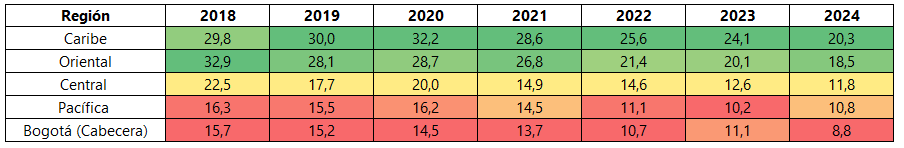
\includegraphics[width=\textwidth]{figura_ipm.png}
\caption{Índice de Pobreza Multidimensional calculado por el DANE}
\label{fig:ipm}
\footnotesize\textit{Fuente: Elaboración propia con datos de \parencite{DANE2024b}.}
\end{figure}

Al desagregar las variables de pobreza por departamento (Figura~\ref{fig:variables_pobreza}), las que más pesan son el bajo logro educativo, la inadecuada eliminación de excretas, el rezago escolar y el trabajo informal \parencite{DANE2024b}. Los hogares tienen en promedio 3,5 integrantes y el 57,2\% reporta que sus ingresos no alcanzan para cubrir los gastos mínimos. En ese contexto es donde llega un proyecto de normalización.

\begin{figure}[H]
\centering
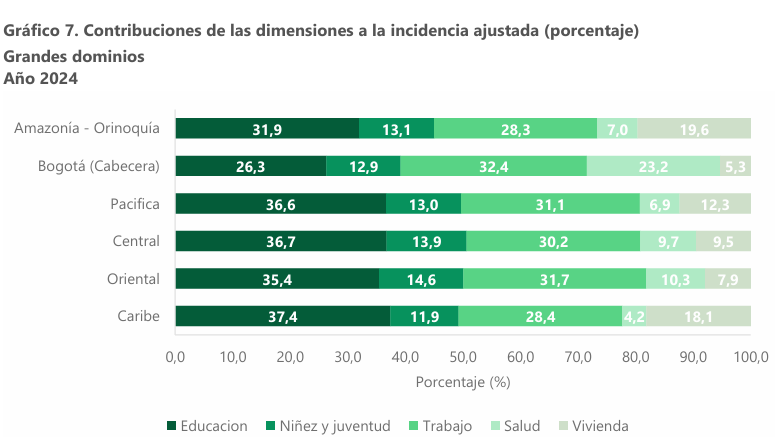
\includegraphics[width=0.75\textwidth]{figura_variables_pobreza.png}
\caption{Variables que contribuyen a la pobreza en la región Caribe en 2024}
\label{fig:variables_pobreza}
\footnotesize\textit{Fuente: Extraído de \parencite{DANE2024b}.}
\end{figure}

Para una familia donde más de la mitad de los ingresos no cubre los gastos básicos, la llegada de una factura de energía que antes no existía o era mínima no es un ajuste menor. Es un choque económico real, y cualquier diseño de intervención que no lo reconozca va a encontrar resistencia.

\subsection{Características habitacionales de los BS}
\label{subsec:habitacionales}

Los BS se construyen sobre la urgencia, no sobre la planificación. Las viviendas se levantan con materiales no certificados, sin seguir ningún parámetro técnico de habitabilidad, y la disposición del barrio no contempla vías de acceso adecuadas para la circulación (Figura~\ref{fig:barrio_viviendas}) \parencite{SerranoRueda2019, VillagranRomero2022}. Esto tiene consecuencias logísticas directas para los proyectos de normalización: llegar a ciertos sectores con equipos y materiales de obra es costoso y en algunos casos técnicamente restrictivo.

\begin{figure}[H]
\centering
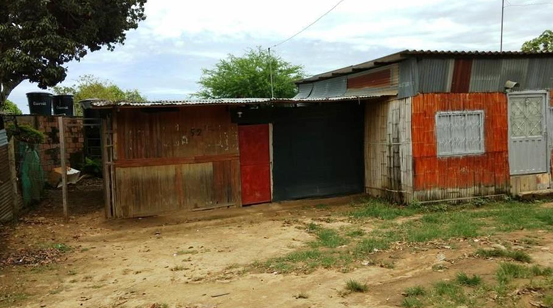
\includegraphics[width=0.48\textwidth]{figura_barrio_viviendas_1.png}\hfill
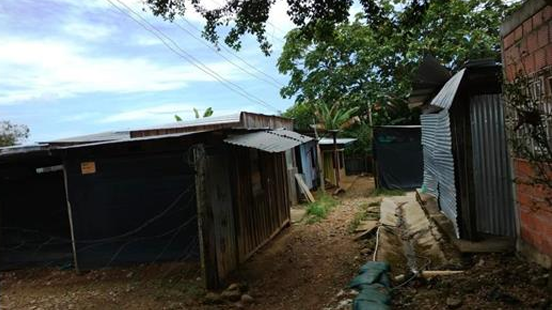
\includegraphics[width=0.48\textwidth]{figura_barrio_viviendas_2.png}
\caption{Barrio subnormal -- Construcción de viviendas}
\label{fig:barrio_viviendas}
\footnotesize\textit{Fuente: Extraído de \parencite{VillagranRomero2022}.}
\end{figure}

\subsection{Estratificación socioeconómica y acceso a subsidios}
\label{subsec:estratificacion}

En 2017, el DNP reclasificó la población colombiana en grupos según ingresos y condiciones sociodemográficas. Los grupos A y B, siendo el grupo A el de menores ingresos y el B el siguiente en la escala, son los de menor capacidad económica. Los BS del Caribe se ubican mayoritariamente en estratos 1 y 2, lo que los hace elegibles para el subsidio del Fondo de Energía Social (FOES), que cubre parte del costo de la energía en áreas especiales. Según la Ley 1117 de 2006, la estratificación es un requisito obligatorio para acceder a ese beneficio \parencite{Ley1117_2006}. Por tanto, para efectos de este estudio, se asume que todos los usuarios de los BS de la región Caribe pertenecen al estrato 1, toda vez que la mayor parte de la subnormalidad en dicha región corresponde a sectores sin estratificación o clasificados en estrato 1.

\subsection{Composición étnica y su incidencia en la normalización}
\label{subsec:etnica}

La región Caribe tiene una presencia significativa de comunidades con diferenciación étnica, y eso importa para los proyectos de normalización. Sus formas de organización, gobernanza y relación con el Estado son distintas a las del resto de la población urbana, y una intervención que no las considera genera fricciones innecesarias. Según el Censo 2018 del DANE, las proporciones con autorreconocimiento étnico en los departamentos seleccionados son \parencite{DANE2018}:

\begin{itemize}
    \item \textbf{Atlántico:} 1,7\% indígena; 2,7\% negro o afrodescendiente.
    \item \textbf{Bolívar:} 0,3\% indígena; 0,2\% palenquero; 6,9\% negro, mulato o afrodescendiente.
    \item \textbf{Magdalena:} 1,7\% indígena; 2,6\% negro, mulato o afrodescendiente.
    \item \textbf{Cesar:} 4,7\% indígena; 3,7\% negro o afrodescendiente.
    \item \textbf{Córdoba:} 13,1\% indígena; 2,3\% afrodescendiente.
    \item \textbf{Sucre:} 12,2\% indígena; 2,8\% afrodescendiente.
    \item \textbf{La Guajira:} 48,4\% indígena; 1,6\% afrodescendiente.
\end{itemize}

La metodología del Capítulo~\ref{chap:metodologia} incorpora esta variable como consideración transversal en la fase de diagnóstico.

\subsection{Niveles de recaudo y cultura de pago}
\label{subsec:recaudo}

Entre el 58\% y el 68\% de los sectores subnormales de Air-e y Afinia registran recaudos de apenas el 1\% al 25\% de la tarifa aplicada. Ese dato no se explica solo por falta de voluntad de pago: es el resultado de limitaciones económicas reales, años de acceso informal al servicio y una desconfianza acumulada hacia el OR y hacia el sistema tarifario.

La consulta a expertos confirma esto con contundencia. El 89,47\% de los profesionales consultados identifica la oposición comunitaria como el principal obstáculo para la normalización. Esa resistencia viene de tres factores que se alimentan mutuamente: el temor a que la factura individual sea más cara de lo que pueden pagar, la desconfianza hacia el OR y la ``cultura del no pago'' que se arraiga cuando el acceso informal lleva décadas siendo la norma \parencite{SerranoRueda2019}.

El temor a la factura tiene base real, pues pasar de no pagar o de pagar una cuota comunitaria de entre \$40.000 y \$50.000 mensuales a una factura individual de \$100.000 a \$200.000 es un salto que no se puede ignorar en el diseño de ningún proyecto. Los expertos consultados lo calificaron de forma casi unánime como un impacto crítico que, si no se maneja bien, puede llevar a los usuarios a volver a las conexiones ilegales. Los detalles de estos resultados se presentan en la Sección~\ref{sec:consulta_expertos} y en el Anexo~\ref{anx:encuesta}.


% ─────────────────────────────────────────────────────────────
\section{Estado de las Redes Eléctricas y Caracterización del Consumo de Energía en Barrios Subnormales}
\label{sec:redes_consumo}
% ─────────────────────────────────────────────────────────────

\subsection{Condiciones técnicas de la infraestructura existente}
\label{subsec:infraestructura}

Las redes eléctricas en los BS de la región Caribe no cumplen el RETIE. No es un incumplimiento puntual: es una situación sistemática que se reproduce en prácticamente todos los asentamientos. Como muestra la Figura~\ref{fig:barrio_red}, la infraestructura se construye de manera artesanal, sin profesionales calificados y sin ningún criterio de planeación técnica. Los problemas más recurrentes son:

\begin{itemize}
    \item Conductores de calibres heterogéneos mezclados en el mismo circuito, sin coordinación de capacidades de corriente.
    \item Sin sistemas de protección coordinados — ni fusibles, ni reconectadores, ni seccionadores.
    \item Acometidas realizadas mediante derivaciones directas sin medición ni protección individual.
    \item Alumbrado público artesanal con luminarias hechizas llamadas coloquialmente ``jeringas''.
    \item Conductores sostenidos con amarres informales en postes de madera, sin respetar las distancias de seguridad del RETIE.
    \item Separación entre postes irregular, sin cálculo de carga del vano ni resistencia mecánica del apoyo.
\end{itemize}

\begin{figure}[H]
\centering
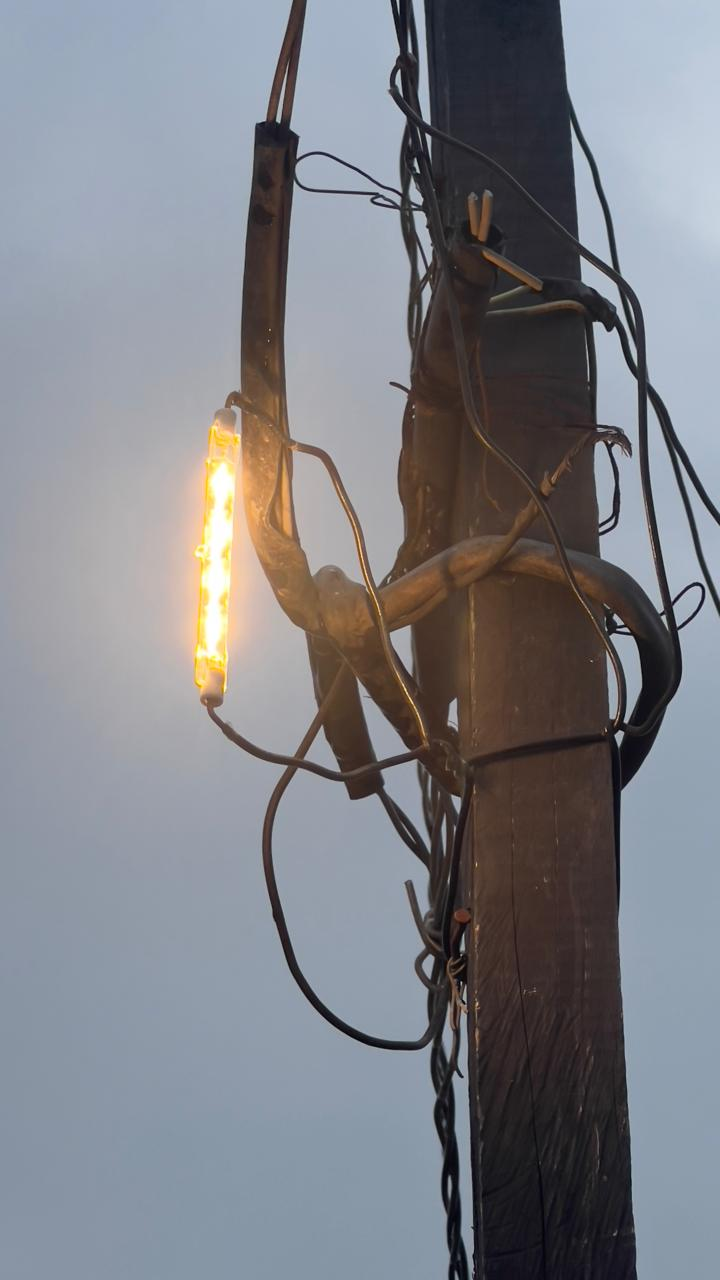
\includegraphics[width=0.30\textwidth]{figura_red_bs_1.png}\hfill
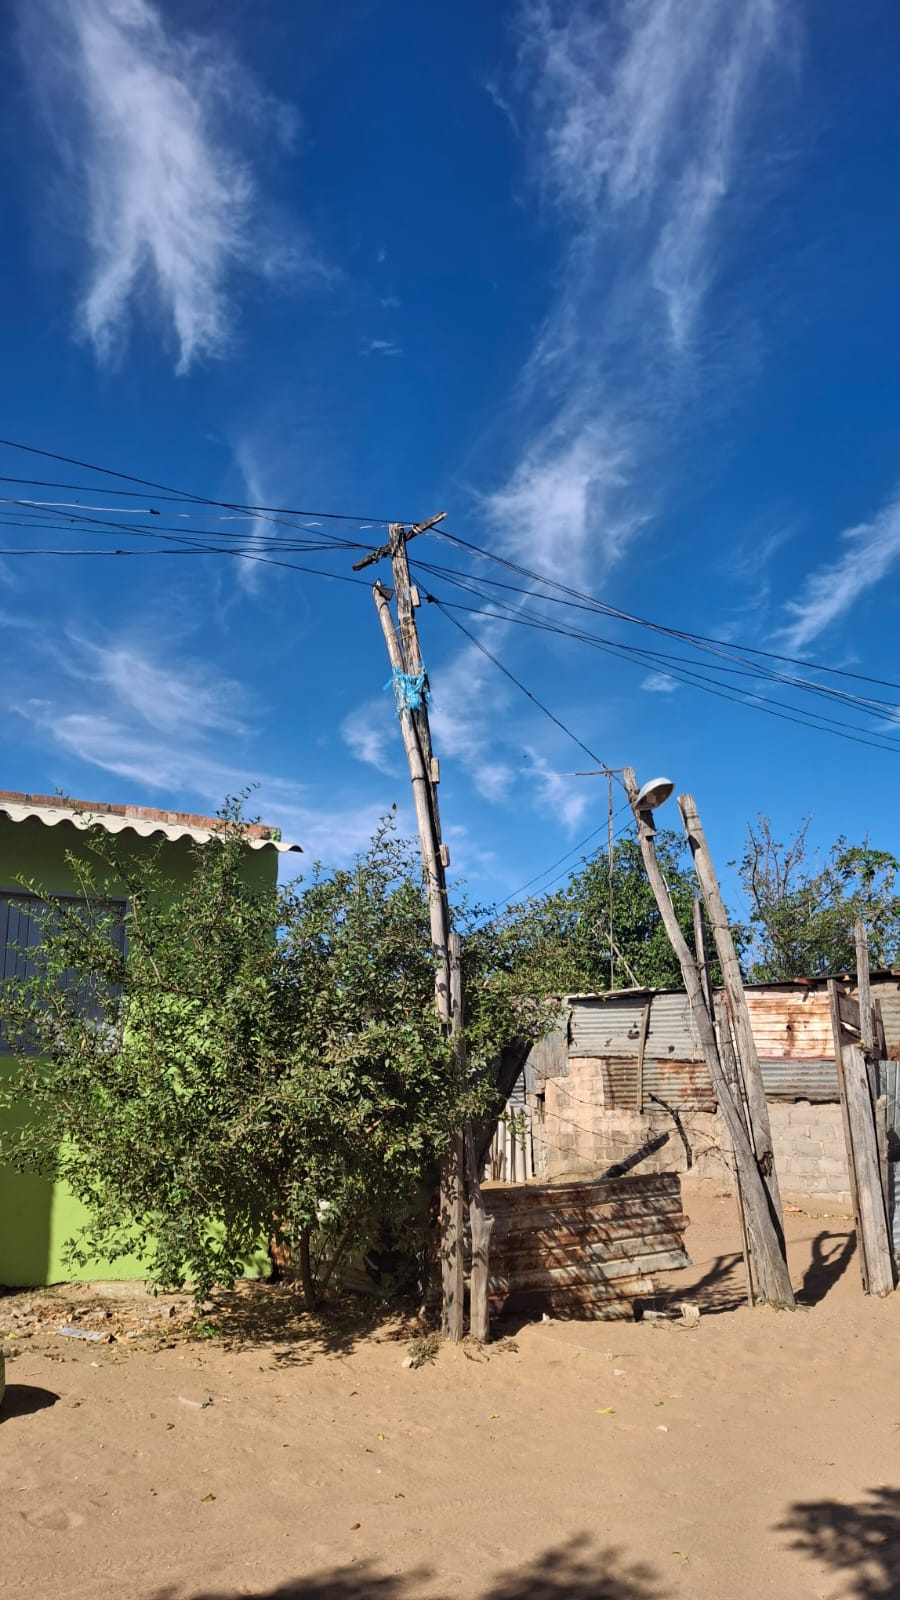
\includegraphics[width=0.30\textwidth]{figura_red_bs_2.png}\hfill
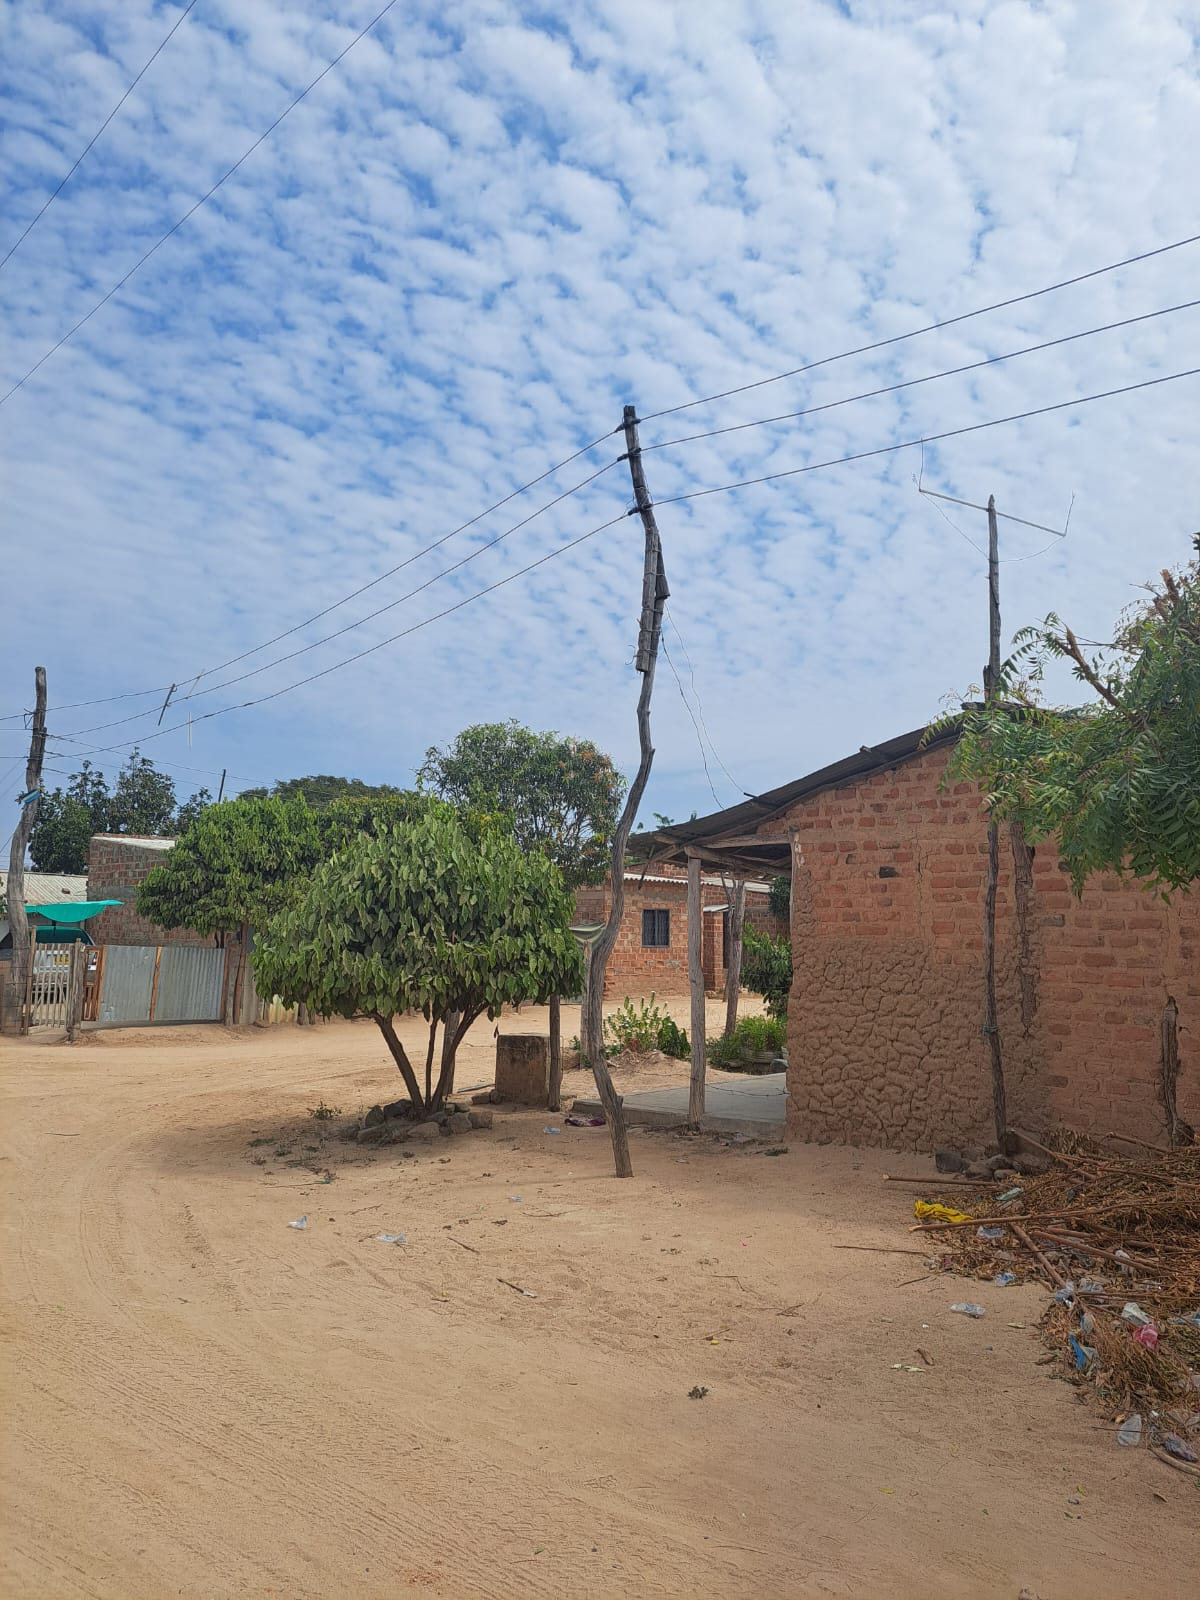
\includegraphics[width=0.36\textwidth]{figura_red_bs_3.png}
\caption{Barrio subnormal -- Construcción de red eléctrica artesanal}
\label{fig:barrio_red}
\footnotesize\textit{Fuente: Autor.}
\end{figure}

El resultado es una red inestable, con alta probabilidad de fallas y un riesgo eléctrico real para quienes viven en el barrio. El riesgo no viene solo de la red exterior: las propias viviendas, muchas veces construidas con materiales inflamables, cuentan con instalaciones internas deficientes que aumentan la probabilidad de incendios y electrocuciones.

El 100\% de los 20 expertos consultados consideró que la normalización es importante para reducir esos riesgos. Las respuestas coinciden en que una red que cumple el RETIE elimina las conexiones inseguras, facilita la inspección y dificulta la manipulación fraudulenta de la infraestructura. Pero varios expertos — E9 y E11 entre ellos — advirtieron que la normalización física no garantiza por sí sola que la red se mantenga en condiciones seguras: si los usuarios reinciden en conexiones ilegales sin que haya seguimiento, los riesgos vuelven. Los datos completos están en la Tabla~\ref{tab:encuesta_red} del Anexo~\ref{anx:encuesta}.

\subsection{Esquema de medición y facturación en áreas especiales}
\label{subsec:medicion}

Sin medidores individuales, la medición se hace a través de macromedidores o totalizadores comunitarios, bajo los esquemas diferenciales de facturación previstos en el DUR 1073 de 2015. Esos esquemas permiten proyecciones de consumo basadas en cargas contratadas o consumos históricos de usuarios similares, con porcentajes de participación donde la responsabilidad de la facturación recae en un suscriptor comunitario \parencite{DUR1073_2015, CabralesSanjuan2015, MendezFuentes2013, SSPD2020}.

El problema es que el macromedidor no discrimina. Debido a que el macromedidor es la frontera comercial del barrio, no hay una discriminación del consumo dentro del mismo; ello conlleva que toda la energía entregada en este punto sea facturada para los usuarios, entre estas las pérdidas técnicas de la red interna, el consumo de las conexiones clandestinas, el alumbrado hechizo. Todo eso termina en la factura del suscriptor comunitario, y los usuarios pagan por pérdidas y consumos que no son suyos, lo que genera una percepción de injusticia.

\subsection{Caracterización climática y su incidencia en la demanda energética}
\label{subsec:clima_demanda}

El 54\% de los 195 municipios del área de análisis se ubica en piso térmico cálido seco y el 38\% en cálido húmedo. Solo el 8\% restante corresponde a climas templados y fríos (ver Anexo~\ref{anx:municipios_clima}). En climas cálidos, los ventiladores y los aires acondicionados no son lujos: son necesidades básicas. Las viviendas de los BS, construidas sin ningún criterio de eficiencia térmica ni de construcción sostenible, presentan una mayor demanda de estos equipos en comparación con las viviendas formales.

El PIEC 2024--2028 establece un consumo residencial estándar de \textbf{145~kWh-mes} para clima cálido húmedo y \textbf{110~kWh-mes} para cálido seco \parencite{UPME2025}. La curva de carga diaria de la Figura~\ref{fig:curva_carga} muestra que los picos de demanda en estos climas se concentran en las horas nocturnas.

\begin{figure}[H]
\centering
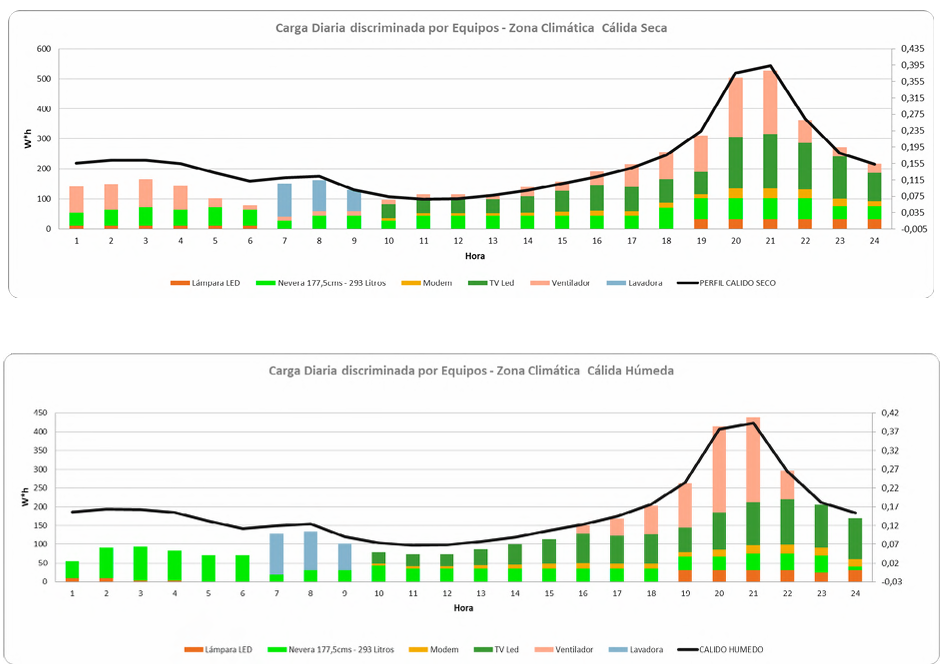
\includegraphics[width=0.85\textwidth]{figura_curva_carga.png}
\caption{Curva de carga diaria; piso térmico cálido seco y húmedo}
\label{fig:curva_carga}
\footnotesize\textit{Fuente: Extraído de \parencite{UPME2025}.}
\end{figure}

\subsection{Consumo real en los BS versus proyecciones estándar}
\label{subsec:consumo_real}

Para conocer el consumo real dentro de los BS — no el estándar del PIEC — se procesaron los datos de la plataforma O3 de la SSPD con los siguientes filtros:

\begin{itemize}
    \item Departamentos de la región Caribe.
    \item Municipios con reportes de suscriptores de Air-e y Afinia.
    \item Pisos térmicos cálido húmedo y cálido seco.
    \item Usuarios residenciales de estrato 1.
    \item Municipios con pago del subsidio FOES.
    \item Periodo: 2023--2025.
\end{itemize}

Los resultados, presentados en el Anexo~\ref{anx:consumo_sspd}, muestran una brecha importante con los estándares. En piso térmico \textbf{cálido húmedo}, el consumo promedio fue de \textbf{235~kWh-mes} (2023), \textbf{232~kWh-mes} (2024) y \textbf{228~kWh-mes} (2025): entre el 61\% y el 62\% más que el estándar del PIEC para ese clima. En piso térmico \textbf{cálido seco}, los registros fueron \textbf{218~kWh-mes} (2023), \textbf{214~kWh-mes} (2024) y \textbf{211~kWh-mes} (2025): entre el 92\% y el 98\% más que el estándar \parencite{SSPD2025}.

La diferencia se explica por el clima, el uso de equipos de baja eficiencia, las pérdidas por conexiones deficientes y los errores de estimación propios de la medición colectiva. Esto tiene una consecuencia directa para el diseño de los sistemas AGPE: si se dimensionan usando los valores del PIEC, van a quedar subdimensionados respecto al consumo real, y el ahorro en factura que se le promete al usuario no va a materializarse. El Capítulo~\ref{chap:tecnico} usa estos valores reales como parámetros de base.


% ─────────────────────────────────────────────────────────────
\section{Impacto de las Problemáticas en Usuarios y Operadores de Red}
\label{sec:impacto}
% ─────────────────────────────────────────────────────────────

La subnormalidad eléctrica no es solo un problema técnico de infraestructura. Sus consecuencias son concretas y afectan de formas distintas a las comunidades, a los OR y a la infraestructura y sostenibilidad del sistema eléctrico de la región.

\subsection{Impacto en la integridad física de las personas}
\label{subsec:impacto_fisico}

Una red sin protecciones, con conexiones informales y en viviendas construidas con materiales inflamables es, antes que todo, un riesgo para la vida. Los cortocircuitos, las sobrecargas, los incendios y los accidentes eléctricos no son eventos hipotéticos en los BS: son consecuencias documentadas de esas condiciones. Quienes intentan realizar conexiones fraudulentas sin conocimiento técnico se exponen a descargas eléctricas y caídas de altura sin ninguna medida de protección.

El 100\% de los expertos consultados confirmó que la normalización es importante para reducir esos riesgos. Varios con experiencia de campo señalaron que la mejora en las condiciones de seguridad es el primer beneficio que los usuarios perciben y valoran después de una normalización, incluso antes de ver cambios en la continuidad del servicio.

\subsection{Impacto en la calidad y continuidad de la prestación del servicio}
\label{subsec:impacto_calidad}

La regulación vigente no exige a los OR cumplir metas de calidad y continuidad dentro de los BS; su responsabilidad formal termina en el macromedidor \parencite{VillagranRomero2022}. Al interior de los BS la red interna presenta condiciones precarias, y los números de la región Caribe ya de por sí son críticos: Afinia registra un SAIFI superior a 43,3 interrupciones anuales y un SAIDI que supera las 72,2 horas promedio al año; Air-e se ubica en rangos de 28,6 a 43,3 interrupciones y 49,5 a 72,2 horas, cifras que dentro de los BS son aún peores \parencite{XM2024}.

Los expertos consultados son matizados en este punto. La mayoría confirma que los usuarios perciben la mejora después de la normalización principalmente a través de menos cortes y menos daños a electrodomésticos. Pero E4 y E9 advierten que esa percepción es frágil: si la calidad no mejora de manera sostenida o si el OR desaparece del barrio después de terminar las obras, la percepción se vuelve negativa, aunque se hayan presentado mejoras técnicas reales que el usuario no pueda identificar o entender a nivel individual o colectivo.

\subsection{Impacto económico y financiero}
\label{subsec:impacto_economico}

Las pérdidas del BS se reflejan principalmente en el componente de Pérdidas Reconocidas (PR) de la tarifa, que en la región Caribe alcanza valores muy por encima del promedio nacional, particularmente para el caso de dicha región. En 2023, el promedio nacional fue de \textbf{\$80,02/kWh}, mientras que Air-e registró \textbf{\$209,43/kWh} y Afinia \textbf{\$176,57/kWh} — un 161\% y un 120,7\% por encima de la media, respectivamente \parencite{UPME2025}. Ese exceso lo pagan todos los usuarios de la región, normalizados o no.

El Régimen Transitorio Especial del artículo 318 de la Ley 1955 de 2019 habilitó a estos OR a trasladar un mayor porcentaje de pérdidas al usuario final durante cinco años, condicionado a que reflejara las inversiones realizadas \parencite{Ley1955_2019}. El efecto paradójico fue encarecer el servicio precisamente en la región donde los usuarios tienen menor capacidad de pago.

Para el OR, el impacto se materializa en cartera de difícil recuperación. Con tasas de recaudo de entre el 1\% y el 25\% en la mayoría de los sectores subnormales, el OR asume el costo de la energía consumida sin poder recuperarla. Ese hueco fiscal reduce la capacidad de inversión en los planes quinquenales y deteriora progresivamente la infraestructura — un círculo que perjudica a todos.

\subsection{Impacto en el desarrollo territorial}
\label{subsec:impacto_territorial}

La normalización eléctrica no es solo energía. \textcite{MosqueraNoguera2005} documentan que la normalización del servicio eléctrico es el primer paso que habilita la llegada de otros servicios urbanos a un asentamiento. El experto E12 lo describe con precisión a partir de su experiencia: cuando un barrio se normaliza, \textit{``una vez que la energía eléctrica se presta en condiciones regulares, pueden comenzar a llegar otras entidades y servicios como los de acueducto y gas, fortaleciendo el desarrollo integral de la comunidad''}. La factura eléctrica se convierte en el primer documento que acredita la existencia de la familia en el sistema de información del Estado, lo que le permite acceder a programas sociales.


% ─────────────────────────────────────────────────────────────
\section{Consulta a Expertos: Perspectivas del Sector sobre la Normalización}
\label{sec:consulta_expertos}
% ─────────────────────────────────────────────────────────────

Para complementar el diagnóstico con información que la literatura técnica no captura fácilmente, se diseñó y aplicó una encuesta a 20 profesionales del sector eléctrico y del sector público con experiencia directa en proyectos de normalización.

\subsection{Descripción del instrumento y perfil de los expertos}
\label{subsec:instrumento}

El instrumento combinó preguntas de escala Likert y preguntas de respuesta abierta, todas de obligatoria respuesta. Se aplicó en un formulario de Google Forms para facilitar la participación de profesionales distribuidos por todo el país. El objetivo fue identificar, desde la experiencia de quienes trabajan en esto, qué tan efectivos son los proyectos de normalización, cómo los perciben los usuarios y qué cuellos de botella se repiten. La ficha técnica completa está en la Tabla~\ref{tab:ficha_tecnica} del Anexo~\ref{anx:encuesta}.

Los 20 expertos — identificados como E1 a E20 — tienen perfiles variados: 15 ingenieros eléctricos, 2 administradores públicos, 2 profesionales de ciencias sociales y 1 ingeniero civil. Esa diversidad fue deliberada: los proyectos de normalización no son solo técnicos, y una muestra de puros ingenieros habría perdido perspectiva. El 65\% de los encuestados tiene más de tres años de experiencia en normalización; cuatro de ellos superan los nueve años. El 80\% proviene exclusivamente del sector público, lo cual es coherente con el objeto de estudio: el PRONE es un programa de financiamiento público. El detalle completo del perfil está en la Tabla~\ref{tab:perfil_expertos} del Anexo~\ref{anx:encuesta}.

\subsection{Resultados: Impacto en la red eléctrica y percepción de los usuarios}
\label{subsec:resultados_red}

\textbf{Reducción de pérdidas no técnicas (P7):} La calificación promedio fue 3,4 sobre 5, con distribución heterogénea: cinco expertos dieron el máximo y cinco dieron 2. La reducción de pérdidas no es un resultado automático de la normalización; depende fuertemente del contexto de cada proyecto, en el entendido de que estas también se generan fuera de los BS debido a error en la facturación, manipulación de medidores, sistemas deficientes de medida, fallas administrativas, entre otras.

\textbf{Reducción de fallas MT-BT (P9):} El 45\% reportó haber observado una reducción efectiva de fallas. Igual porcentaje dijo no tener información suficiente para responder, lo que probablemente se debe a que esta información no es de acceso público; la única información disponible respecto a fallas son los indicadores de calidad del servicio.

\textbf{Importancia para reducir accidentes eléctricos (P10):} El 100\% consideró que sí es importante. Las argumentaciones varían: los más técnicos enfatizan el cumplimiento del RETIE; E9 y E11 señalan que la normalización no garantiza que la red se mantenga segura si los usuarios reinciden en conexiones ilegales sin seguimiento posterior.

\textbf{Percepción de los usuarios (P11):} El patrón que reportan los expertos con experiencia de campo es consistente: los usuarios perciben la mejora principalmente a través de menos cortes y menos daños a electrodomésticos. E12 agrega una observación que vale la pena destacar: en algunos casos se le han cobrado al usuario por costos de conexión inicial valores iguales o superiores a \$400.000, lo que incide en que muchas familias opten por no ser normalizadas, esto en el entendido de que el proceso se ha realizado con recursos de los OR.

\subsection{Resultados: Impacto en el recaudo y perspectiva del usuario frente a la facturación individual}
\label{subsec:resultados_recaudo}

\textbf{Mejora en el recaudo tras la individualización (P8):} 13 de 20 expertos creen que la individualización mejora al menos parcialmente el recaudo. Los siete que discrepan señalan que esa mejora depende de la capacidad de pago de los usuarios y de si el OR condona las deudas previas. E11 plantea el caso más frecuente: la normalización produce el tránsito de la subnormalidad a la cartera en normalidad, sin que el recaudo mejore de verdad.

\textbf{Posición del usuario frente a la legalización (P12):} La posición predominante es resistencia o rechazo inicial. La intensidad varía: es más fuerte en los sectores donde la conexión informal lleva más años y donde hay intermediarios con interés económico en mantener el esquema colectivo. E9 resume bien el dilema del usuario: si la calidad mejora de verdad y el costo es manejable, la legalización tiene sentido; si alguna de las dos condiciones falla, la pregunta ``¿para qué me legalizo?'' no tiene respuesta.

\textbf{Impacto del cambio en la factura (P13):} Casi unanimidad: el impacto es crítico, pues pasar de \$0 o de una cuota fija baja a una factura variable de \$100.000--\$200.000 mensuales para usuarios de clima cálido desajusta el presupuesto familiar. E11 advierte sobre el riesgo más serio: si la normalización no viene acompañada de educación sobre eficiencia energética y de revisión de las instalaciones internas, el choque económico puede ser tan fuerte que los usuarios vuelvan a las conexiones ilegales.

\subsection{Resultados: Estrategias para mejorar la acogida y casos documentados}
\label{subsec:resultados_estrategias}

\textbf{Importancia del acompañamiento social (P15):} El hallazgo más rotundo de toda la consulta: los 20 expertos, sin excepción, dieron 5 sobre 5, sin matices, confirmando que el acompañamiento social no es optativo en un proyecto de normalización, sino la condición que determina si lo que se instala se sostiene en el tiempo \parencite{SerranoRueda2019, MendezFuentes2013}.

\textbf{Principal obstáculo (P16):} Tres factores que se refuerzan mutuamente, presentes en prácticamente todas las respuestas:

\begin{enumerate}[label=\roman*)]
    \item El miedo al incremento en la factura, que se intensifica en sectores donde existen suscriptores comunitarios con interés económico en mantener el esquema colectivo.
    \item La desconfianza en el OR, acumulada durante años de percibir un servicio de baja calidad sin posibilidad de reclamación individual.
    \item La desinformación sobre qué implica la normalización y sobre los derechos y deberes de los usuarios frente al servicio de energía eléctrica, que actores interesados en mantener el esquema actual aprovechan para generar oposición organizada.
\end{enumerate}

\textbf{Estrategias complementarias (P14):} Las más frecuentes son la socialización previa con información clara, el acompañamiento durante las obras, la condonación o refinanciación de deudas históricas y el seguimiento post-normalización. Ningún experto cree que una sola estrategia sea suficiente: la mayoría seleccionó tres o más estrategias combinadas.

\textbf{Casos documentados (P17):} Las experiencias de primera mano que compartieron los expertos ilustran bien lo que funciona y lo que no:

\begin{itemize}
    \item \textbf{Nariño -- CEDENAR} (E5): impacto positivo. El acompañamiento social durante la implementación fue el factor determinante. Hubo resistencia inicial por el incremento en la factura, pero se superó.

    \item \textbf{Isla Fuerte, Córdoba -- 2018} (E9): impacto mixto. El sistema híbrido funcionó bien técnicamente, pero un grupo de usuarios reclamó servicio gratuito porque el Estado los había conectado. El problema fue la brecha entre el beneficio del servicio y la aceptación del esquema de pago, agravada por la falta de claridad previa sobre las reglas tarifarias.

    \item \textbf{Patia -- Cauca} (E4): fracaso. La causa fue un proceso pedagógico insuficiente antes de la intervención.

    \item \textbf{Brisas del Venado} (E17): la comunidad bloqueó la instalación de medidores AMI, argumentando que el sistema de telelectura representaba una intromisión en su privacidad.

    \item \textbf{Costa Caribe -- varios proyectos PRONE} (E1, E15): resultados negativos recurrentes, atribuidos a desinformación, demoras en la ejecución y oposición comunitaria que en algunos casos llevó a la cancelación completa del proyecto.

    \item \textbf{Electrohuila} (E13): experiencia positiva en campañas de legalización, con mejora en pérdidas y recaudo.

    \item \textbf{Caquetá} (E20): caso de éxito, en contraste con fracasos en la costa Caribe. El factor determinante fue el esquema de medición adoptado.
\end{itemize}

\subsection{Síntesis de hallazgos de la consulta}
\label{subsec:sintesis_consulta}

Los hallazgos de la consulta que se integran directamente a la metodología del Capítulo~\ref{chap:metodologia} son seis:

\begin{enumerate}[label=\textbf{\arabic*.}, leftmargin=1.5cm, itemsep=8pt]

    \item La normalización es reconocida como necesaria por todos los actores del sector, pero su éxito no depende principalmente de la calidad técnica de la infraestructura.

    \item El acompañamiento social es condición necesaria, no componente accesorio. Los 20 expertos lo calificaron con 5/5. No presentar al PRONE un proyecto con un componente robusto de gestión social aumenta la probabilidad de fracaso en la ejecución.

    \item El principal obstáculo no es técnico, sino el miedo al incremento en la factura y la desconfianza en el OR. Cualquier estrategia que no aborde esto directamente tiene altas probabilidades de no cumplir con sus objetivos.

    \item El impacto tarifario puede generar reincidencia en la subnormalidad. Eso fundamenta técnica y socialmente la inclusión del AGPE: al reducir el consumo neto de la red, modera el choque económico de la transición.

    \item La medición inteligente (AMI) es técnicamente deseable, pero necesita gestión social especializada.

    \item Los patrones de fracaso en la región Caribe son sistémicos. La combinación de pobreza extrema, informalidad arraigada, los altos consumos de energía que aseguran un confort térmico y la desconfianza institucional acumulada exige estrategias diferenciadas respecto a otras regiones del país.

\end{enumerate}
% ============================================================
%  capitulo3_normativo.tex
%  Capítulo 3: Marco Normativo y Casos de Estudio en Colombia
% ============================================================

\chapter{Marco Normativo y Casos de Estudio en Colombia}
\label{chap:normativo}

El marco normativo que regula la normalización de redes eléctricas en Colombia lleva más de tres décadas construyéndose, respondiendo a aprendizajes de campo, a las necesidades del sector y, más recientemente, a los compromisos del PND 2022--2026 con la transición energética. Entender esa trayectoria ayuda a explicar por qué el esquema actual tiene las oportunidades que tiene, pero también los vacíos que tiene.

Este capítulo cubre tres bloques: la regulación asociada a la normalización de redes, la regulación de los sistemas AGPE, y los casos de estudio documentados en Colombia. Los tres son necesarios para el análisis técnico del Capítulo~\ref{chap:tecnico} y para la metodología del Capítulo~\ref{chap:metodologia}.


% ─────────────────────────────────────────────────────────────
\section{Evolución Normativa Asociada a la Normalización de Redes Eléctricas}
\label{sec:normativa_normalizacion}
% ─────────────────────────────────────────────────────────────

\subsection{Las leyes fundacionales del sector eléctrico colombiano (1994)}
\label{subsec:leyes_1994}

El punto de partida es 1994. Las \textbf{Leyes 142 y 143} establecieron los principios sobre los que todavía opera el sector eléctrico colombiano \parencite{Ley142_1994, Ley143_1994}.

La \textbf{Ley 142} definió los criterios de prestación de los servicios públicos domiciliarios: eficiencia, continuidad, calidad, solidaridad. En lo que respecta a los BS, su artículo 9 es claro: los usuarios tienen derecho a recibir un servicio medido con instrumentos adecuados y a que el consumo facturado sea real. El artículo 11 obliga a las empresas prestadoras a facilitar a los usuarios de menores ingresos el acceso a los subsidios disponibles. Esos subsidios cubren el 50\%, 40\% y 15\% del consumo básico de subsistencia para los estratos 1, 2 y 3 respectivamente, financiados con aportes del 20\% de los estratos 5, 6 y el sector comercial e industrial \parencite{Ley142_1994}.

La \textbf{Ley 143} complementó este marco para el sector eléctrico específicamente. Su artículo 11 definió el consumo básico de subsistencia como la cantidad mínima de electricidad mensual que un usuario típico necesita para satisfacer sus necesidades básicas. El artículo 48 ordenó al Gobierno Nacional destinar recursos del PND a programas de energización prioritarios para lograr cobertura igualitaria en el país. El artículo 66 estableció el ahorro y la eficiencia energética como objetivos del sector \parencite{Ley143_1994}.

\subsection{La creación del PRONE (2003--2006)}
\label{subsec:creacion_prone}

El PRONE nació en el PND 2003--2006, aprobado por la \textbf{Ley 812 de 2003}, que en su artículo 63 lo creó como instrumento de financiamiento para la normalización de redes eléctricas \parencite{Ley812_2003}. Tres años después, la \textbf{Ley 1117 de 2006} le dio soporte legal definitivo y lo constituyó formalmente como un fondo administrado por el MME, con el propósito de financiar planes, programas y proyectos para legalizar usuarios\footnote{La legalización es el proceso de individualizar la medida, crear el código de usuario en el sistema del OR y establecer la relación contractual con factura individual.} y adecuar las redes en los BS del SIN \parencite{Ley1117_2006}.

La reglamentación detallada llegó con el \textbf{DUR 1073 de 2015}, artículo 2.2.3.3.3.1.1, que delimitó los rubros financiables dentro del programa: \textit{``únicamente el suministro e instalación de las redes de distribución, los transformadores de distribución, las acometidas a las viviendas de los usuarios y los medidores o sistema de medición del consumo. En lo referente al desmonte del material existente [\ldots] su costo no podrá superar el tres por ciento (3\%) del valor total del proyecto''} \parencite{DUR1073_2015}.

El DUR también define quiénes pueden presentar proyectos, los requisitos mínimos, los criterios de priorización y las condiciones de propiedad de los activos una vez terminadas las obras. Es el marco institucional vigente dentro del cual se rigen los OR que buscan financiamiento público para la normalización de redes eléctricas.

Adicionalmente, consolida la reglamentación del \textbf{FOES}, subsidio para usuarios de estratos 1 y 2 en áreas especiales. Su aplicación depende del consumo de subsistencia definido por la UPME, del porcentaje de recaudo del OR —la cobertura del subsidio varía entre el 40\% y el 100\% según ese indicador— y de la certificación anual del área especial ante la SSPD \parencite{DUR1073_2015}.

El mecanismo de financiamiento del PRONE quedó fijado por la \textbf{Ley 1753 de 2015}: el fondo recibe \$1,90 por kilovatio hora transportado en el SIN a través del ASIC. El FOES, por su parte, cubre hasta \$92 por kilovatio hora destinado al consumo de subsistencia de los estratos 1 y 2 \parencite{Ley1753_2015}.

\subsection{Los esquemas diferenciales de facturación}
\label{subsec:esquemas_diferenciales}

El DUR 1073 reconoce algo que en la práctica resulta evidente: las reglas convencionales de facturación no funcionan en los BS. Por eso establece esquemas alternativos que los OR pueden usar: medición y facturación comunitaria, proyecciones de consumo basadas en cargas contratadas o históricos, pago anticipado y periodos de facturación flexibles \parencite{DUR1073_2015}.

Para aplicar cualquiera de estos esquemas, el OR debe firmar contratos con suscriptores comunitarios que definan cómo se mide, cómo se factura y cómo se paga. El problema práctico es que el suscriptor comunitario no tiene herramientas legales reales para exigir el pago a los usuarios individuales.

\subsection{La Resolución CREG 015 de 2018 y la remuneración de la distribución}
\label{subsec:resolucion015}

La \textbf{Resolución 015 de 2018} de la CREG estableció la metodología para remunerar la actividad de distribución en el SIN \parencite{ResolucionCREG015_2018}. Los capítulos 6 y 7 —sobre planes de inversión y gestión de pérdidas— son los más relevantes para este trabajo: definen cómo se remunera vía tarifa la inversión orientada a reducir pérdidas, mejorar calidad y aumentar demanda.

\subsection{La incorporación del AGPE al PRONE (2023--2024)}
\label{subsec:agpe_prone}

El cambio normativo más importante en los veinte años de historia del PRONE llegó con el \textbf{PND 2022--2026}, aprobado por la \textbf{Ley 2294 de 2023}: por primera vez, los recursos del programa pueden destinarse a financiar sistemas AGPE dentro de los proyectos de normalización \parencite{Ley2294_2023}.

La reglamentación vino con el \textbf{Decreto 1023 de 2024}, que adicionó la Subsección 3.4 al DUR 1073. El decreto fijó los requisitos para presentar proyectos con AGPE, los criterios de priorización y las reglas de propiedad de los activos \parencite{Decreto1023_2024}. Una novedad relevante: los activos de generación construidos con recursos del PRONE pueden transferirse a los usuarios beneficiados a través de la figura de \textbf{Comunidades Energéticas}, reglamentadas por el \textbf{Decreto 2236 de 2023}, que les otorga carácter legal de prestador de servicio público \parencite{Decreto2236_2023, DUR1073_2015}.

El \textbf{Decreto 1403 de 2024} amplió las posibilidades técnicas al permitir que un sistema AGPE entregue excedentes al SIN o consuma energía en sitios distintos a los de producción \parencite{Decreto1403_2024}.

La primera convocatoria con el AGPE como gasto elegible fue la \textbf{Resolución 40243 de 2025} \parencite{ResolucionMME40243_2025}. El resultado fue elocuente: ninguno de los proyectos presentados cumplió con todos los requisitos del MME \parencite{MME2025}. Ese dato confirma, de la manera más directa posible, la brecha metodológica que esta monografía busca cerrar.


% ─────────────────────────────────────────────────────────────
\section{Evolución Normativa Asociada a los Sistemas de AGPE}
\label{sec:normativa_agpe}
% ─────────────────────────────────────────────────────────────

\subsection{Los orígenes restrictivos de la autogeneración (1994--2014)}
\label{subsec:origenes_agpe}

La \textbf{Ley 143 de 1994} definió al autogenerador como \textit{``aquel generador que produce energía eléctrica exclusivamente para atender sus propias necesidades''} \parencite{Ley143_1994}. Era autoconsumo puro, sin posibilidad de excedentes, sin red comunitaria y sin articulación con la política energética.

La \textbf{Resolución 84 de 1996} reglamentó eso con un esquema aún más restrictivo: el autogenerador conectado al SIN no podía vender excedentes, salvo en situaciones de racionamiento y solo a través de la Bolsa de Energía. La conexión al sistema se concebía exclusivamente como respaldo. Para los usuarios regulados, el suministro iba obligatoriamente a través del comercializador del área; los no regulados podían contratar libremente.

\subsection{La Ley 1715 de 2014: el cambio estructural}
\label{subsec:ley1715}

La \textbf{Ley 1715 de 2014} cambió las reglas de fondo \parencite{Ley1715_2014}. Incorporó las FNCER a la política energética nacional y redefinió la autogeneración: dejó de ser exclusivamente autoconsumo y pasó a reconocerse como una alternativa con posibilidad de entregar excedentes a la red bajo condiciones que definiría la CREG.

Los beneficios que trajo son concretos: incentivos tributarios para proyectos con FNCER (exención de IVA, deducción de renta, exención de aranceles), reconocimiento de la autogeneración como instrumento de eficiencia energética y posibilidad de medición bidireccional. Ese último punto es técnicamente fundamental: sin medición bidireccional no hay forma de contabilizar lo que el sistema inyecta a la red.

Entre 2014 y 2018 la normativa reglamentaria fue tomando forma. La \textbf{Resolución UPME 281 de 2015} fijó el límite de 1~MW para los AGPE \parencite{ResolucionUPME281_2015}. El \textbf{Decreto 348 de 2017} simplificó las condiciones de medición, conexión y contrato de respaldo \parencite{Decreto348_2017}. La \textbf{Resolución CREG 030 de 2018} fue el primer intento integral de regular los AGPE en el SIN \parencite{ResolucionCREG030_2018}, pero generó tantas preguntas de aplicación que la CREG tuvo que revisarla.

\subsection{La Resolución CREG 174 de 2021: la norma vigente}
\label{subsec:resolucion174}

La \textbf{Resolución CREG 174 de 2021} derogó completamente la 030 de 2018 y es hoy la referencia regulatoria para los sistemas AGPE en el SIN \parencite{ResolucionCREG174_2021}. Tres cambios son particularmente relevantes para proyectos en BS:

\begin{itemize}
    \item \textbf{El límite de inyección subió del 15\% al 50\%} de la capacidad del transformador o circuito al que se conecta el AGPE. Para los circuitos que sirven a los BS, que generalmente tienen capacidades nominales relativamente bajas, el umbral anterior del 15\% limitaba significativamente la potencia instalable del sistema AGPE sin requerir refuerzos en la red. Con el nuevo límite del 50\%, la potencia de generación que puede conectarse al mismo punto aumenta considerablemente, lo que mejora la viabilidad técnica y económica de estos proyectos al permitir sistemas de mayor tamaño sin inversiones adicionales en infraestructura de red.

    \item \textbf{La información de conexión se hizo más accesible.} La resolución obligó a los OR a mantener un micrositio específico en su página web donde cualquier interesado puede consultar las características técnicas del punto de conexión y el estado de la red, sin software adicional. Eso reduce una barrera real para quien está formulando un proyecto.

    \item \textbf{Se definió el manejo de excedentes vía tarifa}, distinguiendo el caso en que los excedentes inyectados a la red superan la energía importada desde ella (denominado permuta: el AGPE entrega más energía de la que toma, y el OR compensa al usuario a una tarifa definida por la CREG) del caso en que los excedentes son menores o iguales a las importaciones (el excedente se descuenta directamente de la factura). Esa distinción alinea la regulación con la realidad técnica de la medición bidireccional y define cómo se liquida el intercambio de energía entre el usuario y el OR.
\end{itemize}

\subsection{La integración del AGPE en la normalización (2023--2025)}
\label{subsec:integracion_agpe_normalizacion}

El Decreto 1023 de 2024 es la pieza normativa que hace posible lo que propone esta monografía. Integra el AGPE dentro del PRONE y crea la distinción de propiedad que ya se mencionó: la red normalizada queda bajo el OR para efectos de AOM; los activos de generación pueden transferirse a la Comunidad Energética. Esa distinción tiene consecuencias sobre quién responde por qué en el largo plazo, y requiere que el proyecto la defina con claridad desde el inicio \parencite{Decreto1023_2024}.

El costo unitario por usuario en proyectos con AGPE es notablemente superior al de proyectos convencionales. Los 30 proyectos de la vigencia 2025 lo ilustran: requirieron un valor de financiación significativamente mayor al de vigencias anteriores con muchos más proyectos \parencite{MME2025}. Esa presión sobre los recursos disponibles del PRONE refuerza la necesidad de criterios de priorización más específicos para proyectos con AGPE, uno de los vacíos regulatorios que se aborda en el Capítulo~\ref{chap:metodologia}.


% ─────────────────────────────────────────────────────────────
\section{Análisis de la Normalización Eléctrica en Colombia: Experiencias, Financiación y Cuellos de Botella}
\label{sec:casos_estudio}
% ─────────────────────────────────────────────────────────────

Tres décadas de proyectos de normalización en Colombia dejan un registro valioso. Esta sección analiza los tres casos con mayor documentación disponible en la literatura, y, de manera complementaria, se analizó el comportamiento histórico de los proyectos del PRONE entre 2005 y 2025.

\subsection{Caso 1 -- Cartagena, Bolívar (1991)}
\label{subsec:caso_cartagena}

En 1991, la Electrificadora de Bolívar evaluó la viabilidad de construir redes de distribución en zonas subnormales de Cartagena usando el método de normalización por tramos secundarios, siendo uno de los primeros estudios documentados de este tipo en el país \parencite{CastilloQuintana1991}.

El diseño propuesto era sencillo: un vano de 80~m de red primaria (13,2~kV) y dos vanos de 40~m de red secundaria (220~V), con postes de 12~m y 8~m ubicados en calles principales. Se distinguía entre usuarios directos —más cerca de la calle, con alumbrado público, facturación sobre el 100\% del consumo— e indirectos —más alejados, sin alumbrado, con recaudo sobre el 50\% a través de la JAC—. Se esperaba beneficiar a 24 usuarios directos y 18 indirectos. La financiación proyectada era mediante créditos del BID y la FEN, con recuperación de inversión en 18 meses.

El caso tiene varias limitaciones estructurales que, tres décadas después, siguen siendo completamente relevantes. El modelo colectivo dividía el consumo por partes iguales sin reconocer el ahorro individual, lo que no incentivaba el uso racional de la energía. La brecha entre usuarios directos e indirectos generaba inequidades concretas en acceso al alumbrado y disponibilidad de potencia. Y los usuarios ya entonces declaraban destinar el 80\% de sus ingresos a necesidades básicas, lo que ponía en duda la capacidad real de pago sobre la que se sostenía el modelo financiero \parencite{CastilloQuintana1991}.

\subsection{Caso 2 -- Sabana de Torres, Santander (2010--2014)}
\label{subsec:caso_santander}

La Electrificadora de Santander (ESSA) ejecutó entre 2010 y 2014 uno de los proyectos de normalización más completos ejecutados en el país, orientado a reducir pérdidas no técnicas que en 2009 representaban aproximadamente el 20\% de la energía transportada \parencite{MendezFuentes2013}.

La inversión fue íntegramente con recursos propios del OR, distintos de los recursos públicos del Ministerio que provienen del presupuesto general de la nación: \$114.885 millones en total, de los cuales \$38.894 millones fueron inversión directa en infraestructura y \$75.991 millones costos operativos. La estrategia técnica combinó tres componentes:

\begin{enumerate}[label=\roman*), leftmargin=2cm, itemsep=4pt]
    \item \textbf{Red Chilena:} En lugar de red de baja tensión convencional, se instalaron transformadores pequeños de 5 a 15~kVA que alimentan directamente entre 6 y 9 usuarios a través de la acometida, desde una caja de derivación. Sin red de BT, no hay dónde conectarse ilegalmente.

    \item \textbf{Conductor blindado antifraude:} Se sustituyó el trenzado por cable concéntrico TRI y TETRA CAPA, que no puede ser perforado con los conectores informales que se usaban para las conexiones clandestinas. El conductor del alumbrado público también se redujo de calibre (a cable 2×18) para que solo tuviera capacidad para las luminarias.

    \item \textbf{AMI en modalidad prepago:} Los medidores no se instalaron dentro de las viviendas para evitar manipulaciones; solo se dejaron displays de visualización en el interior. El objetivo era desincentivar el fraude sin perder la transparencia hacia el usuario.
\end{enumerate}

Al cierre de 2013 se habían ejecutado 38.285 legalizaciones y normalizado 110.064 usuarios en total \parencite{MendezFuentes2013}. Los resultados son sólidos. Sin embargo, la lección más importante es sobre escala: una inversión de \$114.885 millones con recursos propios está fuera del alcance de la mayoría de los OR del país, especialmente de los que operan en el Caribe con los problemas financieros documentados en el Capítulo~\ref{chap:diagnostico}. Vale precisar que el costo por usuario del PRONE actualmente se estima alrededor de \$11 millones, lo que representa un esquema de financiamiento más accesible para los OR de menor tamaño. Sin el PRONE, este tipo de proyectos difícilmente sería replicable en el contexto caribeño.

\subsection{Caso 3 -- Popayán, Cauca (2014--2018)}
\label{subsec:caso_popayan}

La experiencia de la Compañía Energética de Occidente (CEO) en Popayán se distingue por la integralidad del proceso: combinó intervención técnica, gestión social sistemática y articulación interinstitucional en un solo proyecto \parencite{SerranoRueda2019}.

En cuatro años se normalizaron 41 asentamientos en Popayán —establecidos por más de 15 años— con 12.000 habitantes. El financiamiento fue mixto: el OR aportó el 76\% del valor total (\$3.500 millones) y el MME el 24\% restante a través del PRONE. Esa estructura muestra algo importante: el PRONE no necesita ser el financiador principal para ser determinante; puede funcionar como el factor que hace viable lo que el OR solo no podría asumir.

La estrategia tuvo tres componentes. El técnico incluyó AMI y modernización completa de la infraestructura de distribución secundaria. El social fue el más intenso: formación comunitaria sistemática sobre derechos y deberes, lectura de factura y uso eficiente de la energía, realizada antes, durante y después de las obras. El componente de eficiencia energética fue el ``Cambiatón'': sustitución masiva de luminarias incandescentes por ahorradoras en las viviendas de los usuarios, para que la transición a la facturación individual no llegara acompañada de un consumo sin reducir.

Los resultados hablan solos: recaudo del 0\% al 97\%, reducción del 67\% en el consumo por usuario (de 197 a 65~kWh-mes), mejora en calidad del servicio y condonación de 15 años de deudas acumuladas. Lo que no se puede ignorar es que articular todo eso requirió más de diez entidades — alcaldía, personería, defensoría, concejo, procuraduría, SSPD, secretarías, fuerza pública y medios de comunicación. Sin esa articulación, los asentamientos con mayor resistencia social no se hubieran podido intervenir \parencite{SerranoRueda2019}.

\subsection{Comportamiento histórico del PRONE (2005--2025)}
\label{subsec:prone_historico}

A partir de las actas CAPRONE y los informes de evaluación del MME se construyó una base de datos de los proyectos adjudicados por vigencia, relacionándose los OR seleccionados, ubicación del proyecto, número de beneficiarios y valor solicitado \parencite{MME2025}. De esta se estableció que la concentración de proyectos financiados por el MME fueron presentados para la región Caribe, Pacífica y algunos departamentos de la andina. En cuanto a Orinoquía y Amazonía la participación fue marginal, lo cual es coherente con la existencia de BS documentados en esa zona.

El 52,03\% de los proyectos presentados entre 2005 y 2025 provienen de la Electrificadora de la Costa Caribe (hoy Afinia y Air-e); en 2024, ningún proyecto de esos OR —ni de ningún otro— resultó elegible.

Entre las variaciones anuales se destacan las siguientes:

\begin{itemize}
    \item \textbf{2007--2010}: Sin proyectos aprobados. El ajuste normativo tras la Ley 1117 de 2006 y el Decreto 1123 de 2008 redefinió actores, condiciones y procedimientos, y el programa estuvo prácticamente detenido.

    \item \textbf{2012}: 185 proyectos, el pico histórico del programa. Probablemente el resultado de años de acumulación de diagnósticos técnicos en los OR.

    \item \textbf{2016--2018}: De nuevo sin proyectos. El DUR 1073 de 2015 generó otro periodo de ajuste institucional.

    \item \textbf{2024}: Cero proyectos elegibles. El primer año con convocatoria bajo el nuevo esquema AGPE y ninguno cumplió los requisitos.

    \item \textbf{2025}: 30 proyectos con el esquema nuevo, beneficiando alrededor de 11.000 usuarios en La Guajira, Magdalena, Atlántico, Nariño, Huila y Meta. El valor de financiación solicitado fue significativamente mayor al de vigencias con mucho más proyectos, por el costo del componente solar.
\end{itemize}

En total, entre 2003 y 2025 el PRONE ha beneficiado aproximadamente a 290.000 usuarios según los proyectos aprobados. Esa cifra puede diferir de los beneficiarios reales por los ajustes que ocurren durante la ejecución.

\begin{table}[H]
\centering
\caption{Casos de estudio de normalización en Colombia con recursos públicos y privados}
\label{tab:casos_estudio}
\begin{tabularx}{\textwidth}{>{\RaggedRight}p{2.5cm}
                             >{\RaggedRight}p{2.8cm}
                             >{\RaggedRight}p{3.2cm}
                             >{\RaggedRight\arraybackslash}p{4.3cm}}
\toprule
\textbf{Caso de Estudio} & \textbf{Financiación / Normatividad} & \textbf{Impacto en los Usuarios} & \textbf{Impacto en el OR} \\
\midrule
\rowcolor{grisclaro}
\textbf{Cartagena, Bolívar} (1991)
& Créditos BID-FEN. Sin regulación sobre PR ni esquemas diferenciales.
& \textit{Negativo:} Usuarios asumían costos de medición y todas las pérdidas. Brecha entre usuarios directos e indirectos.
& \textit{Cuello de botella:} Recaudo delegado a JAC sin herramientas legales. \newline\textit{Positivo:} Proyección de recuperación a 18 meses. \\

\textbf{Sabana de Torres, Santander} (2010--2014)
& Recursos propios del OR (\$114.885 millones).
& \textit{Positivo:} Información en tiempo real (AMI), infraestructura blindada, eliminación de conexiones fraudulentas.
& \textit{Negativo:} Alta inversión, reincidencia en sectores sin seguimiento. \newline\textit{Positivo:} Reducción de pérdidas con Red Chilena. \\

\rowcolor{grisclaro}
\textbf{Popayán, Cauca} (2014--2018)
& Mixta: OR 76\% + PRONE 24\%. Articulación con MME.
& \textit{Positivo:} Consumo redujo 67\%, deudas históricas condonadas, mejora en seguridad y sentido de legalidad.
& \textit{Positivo:} Recaudo 0\% a 97\%, mejora en calidad. \newline\textit{Negativo:} Asumir cartera morosa. \newline\textit{Cuello de botella:} Articulación con más de 10 instituciones. \\
\bottomrule
\multicolumn{4}{l}{\footnotesize\textit{Fuente: Elaboración propia con datos de \parencite{CastilloQuintana1991, MendezFuentes2013, SerranoRueda2019}.}}
\end{tabularx}
\end{table}

\subsection{Lo que enseñan los tres casos}
\label{subsec:sintesis_casos}

Cuatro patrones se repiten con independencia del OR, el periodo o la región:

\textbf{La tecnología no se sostiene sola.} Santander y Popayán muestran que la infraestructura avanzada mejora los resultados técnicos, pero si la comunidad no la apropia, los usuarios encuentran la manera de sortearla. El blindaje más sofisticado no reemplaza al acompañamiento social.

\textbf{La gestión social previa es lo que diferencia el éxito del fracaso.} No el diseño eléctrico. El contraste entre Popayán —con formación comunitaria sistemática— y los proyectos cancelados en el Caribe por oposición organizada lo ilustra de manera directa.

\textbf{El recaudo no mejora solo con la individualización.} La normalización crea las condiciones para mejorar el recaudo, pero no lo garantiza. Depende de la capacidad de pago de los usuarios, de los mecanismos de cobro del OR y de si se condona o no la deuda histórica.

\textbf{Los cuellos de botella más frecuentes son institucionales, no técnicos.} La falta de certificación del BS, la debilidad de algunos OR para estructurar proyectos elegibles y la complejidad de los requisitos del PRONE no se resuelven con mejores equipos de medición. Requieren herramientas metodológicas claras, que es precisamente lo que propone el Capítulo~\ref{chap:metodologia}.
% ============================================================
%  capitulo4_tecnico.tex
%  Capítulo 4: Análisis Técnico y Financiero de la
%              Implementación de AGPE en Normalización
% ============================================================

\chapter{Análisis Técnico y Financiero de la Implementación de AGPE en Normalización}
\label{chap:tecnico}

Este capítulo tiene dos partes. La primera revisa el comportamiento
histórico de la normalización en Colombia desde la perspectiva
financiera, cruzando los datos de inversión privada de Air-e y Afinia
con el registro de proyectos del PRONE entre 2005 y 2025. La segunda
desarrolla el caso de estudio hipotético que evalúa la viabilidad
técnica y financiera de integrar sistemas AGPE en un proyecto de
normalización bajo las condiciones reales de la región Caribe.

Los parámetros de demanda y las condiciones climáticas y
socioeconómicas del caso de estudio vienen del
Capítulo~\ref{chap:diagnostico}. El marco normativo de referencia
está en el Capítulo~\ref{chap:normativo}.


% ─────────────────────────────────────────────────────────────
\section{Normalización a Través de los Años con Recursos Públicos y Privados}
\label{sec:historico}
% ─────────────────────────────────────────────────────────────

La literatura sobre normalización en Colombia documenta poco lo que
pasa en campo. No hay muchos estudios que registren un proyecto desde
la pre-factibilidad hasta la operación con datos suficientes para
analizarlo. Lo que sí hay son los casos del Capítulo~\ref{chap:normativo},
las actas CAPRONE del MME y los informes quinquenales de Air-e y Afinia
para los años 2021--2024. Con eso se construyó este análisis.

\subsection{Comportamiento de la normalización con recursos privados}
\label{subsec:rec_privados}

Los dos casos con inversión privada documentada son los de Santander
(2010--2014) y Cauca (2014--2018), analizados en el
Capítulo~\ref{chap:normativo}. Fuera de esos, hay dos estudios con
datos cuantitativos relevantes.

\textcite{CabralesSanjuan2015} estimaron un costo promedio de
\textbf{\$1.093.052 por usuario} en proyectos de normalización urbana
en CENS, orientados principalmente a la sustitución de medidores y
acometidas obsoletas. Es la referencia numérica más citada en la
literatura para proyectos de este tipo. \textcite{PenaMantilla2020},
por su parte, analizaron alternativas de mitigación de pérdidas en EPM
para el municipio de Itagüí y encontraron que legalizar y controlar
usuarios es más rentable que normalizar completamente la infraestructura,
aunque advierten que sin revisiones y controles posteriores los usuarios
normalizados tienden a reincidir en las conexiones ilegales.

Al revisar los planes quinquenales de Air-e y Afinia, lo que se ve es
una priorización constante de los niveles de tensión 2, 3 y 4. El nivel
1 —que es donde está la infraestructura de los BS— queda relegado.

\subsubsection{Air-e: comportamiento de la inversión 2021--2024}
\label{subsubsec:aire_inversion}

La inversión de Air-e en nivel de tensión 1 fue inferior al 30\% durante
2021--2023: 13\% en 2021, 24\% en 2022 y 27\% en 2023. En 2024 subió al
50\%, pero se destinó a modernizar líneas y circuitos, no a normalizar
BS. Los informes no identifican ninguna partida específica para usuarios
subnormales \parencite{Aire2021, Aire2022, Aire2023, Aire2024}.

Más preocupante aún: la ejecución del plan de inversiones aprobado por
la CREG fue del 25\% en 2023 y del 19\% en 2024. El OR justificó esos
incumplimientos en dificultades operativas y problemas de liquidez. La
conclusión es directa: si Air-e no puede ejecutar ni su propio plan de
inversiones, su capacidad de cofinanciar proyectos de normalización con
recursos propios es prácticamente nula. El PRONE no es un complemento
conveniente para ese OR — es la única vía realista.

\subsubsection{Afinia: estrategias de control de pérdidas 2021--2024}
\label{subsubsec:afinia_perdidas}

Afinia no detalla en sus informes la inversión por nivel de tensión, pero
sí muestra un esfuerzo sostenido en reducción y control de pérdidas
mediante acciones técnicas y comerciales: normalización de medida en
suministros con altas pérdidas, medición prepago, adecuación de redes
internas y talleres de gestión social para mejorar el recaudo
\parencite{Afinia2021, Afinia2022, Afinia2023, Afinia2024}.

La Tabla~\ref{tab:afinia_acciones} muestra las acciones ejecutadas entre
2021 y 2024. Las pérdidas bajaron de 27,69\% en 2021 a 26,15\% en 2022,
pero volvieron a subir en 2023 (26,73\%) y 2024 (27,95\%). El OR
atribuye el rebote al aumento del hurto de energía por la inconformidad
de los usuarios con el alza del Costo Unitario (CU) por encima de
\$1.000/kWh, y al mayor consumo generado por el Fenómeno de El Niño.

\begin{table}[H]
\centering
\caption{Acciones realizadas por Afinia para el control y reducción de pérdidas (2021--2024)}
\label{tab:afinia_acciones}
\begin{tabularx}{\textwidth}{>{\RaggedRight}X
                             >{\centering}p{2cm}
                             >{\centering}p{2cm}
                             >{\centering}p{2cm}
                             >{\centering\arraybackslash}p{2cm}}
\toprule
\textbf{Acción} & \textbf{2021} & \textbf{2022} & \textbf{2023} & \textbf{2024} \\
\midrule
\rowcolor{grisclaro}
Normalización de suministros sin medidor            & 16.841 & 10.580 & 13.260 & 8.487  \\
Suministros con medición inteligente                & 13.738 & 26.723 & ---    & ---    \\
\rowcolor{grisclaro}
Instalación de macromedidores NT1                   & 281    & 740    & 2.739  & 10.851 \\
Incorporación de nuevas invasiones (contratación)   & 86     & 34     & ---    & ---    \\
\rowcolor{grisclaro}
Incorporación de clientes conectados ilícitamente   & 6.145  & 36.866 & 35.118 & 36.774 \\
Normalización de la medida                          & 1.719  & 6.250  & 14.131 & 19.461 \\
\rowcolor{grisclaro}
Instalación de equipos de medida prepago            & 255    & 270    & ---    & ---    \\
\midrule
\textbf{Total}  & \textbf{39.065} & \textbf{81.463} & \textbf{65.248} & \textbf{75.573} \\
\bottomrule
\multicolumn{5}{l}{\footnotesize\textit{Fuente: Elaboración propia
con datos de \parencite{Afinia2021, Afinia2022, Afinia2023, Afinia2024}.}}
\end{tabularx}
\end{table}

La instalación de macromedidores en NT1 pasó de 281 en 2021 a 10.851 en
2024, y la normalización de la medida de 1.719 a 19.461. Hay aprendizaje
y hay escala creciente. Pero el rebote en pérdidas de los últimos dos
años muestra que las estrategias implementadas no son suficientes para
sostener la tendencia. Las limitaciones operativas y financieras siguen
presentes.

\subsection{Comportamiento de la normalización con recursos públicos}
\label{subsec:rec_publicos}

La base de datos construida a partir de las actas CAPRONE del MME
registra, por vigencia, el número de proyectos presentados por OR, el
valor aprobado y los usuarios beneficiarios \parencite{MME2025}. El
archivo complementario \textit{Proyectos adjudicados PRONE 2005--2025}
contiene el detalle completo por municipio y departamento.

Con esa información se construyó el análisis en Power BI que se presenta
en las figuras siguientes.

\begin{figure}[H]
\centering
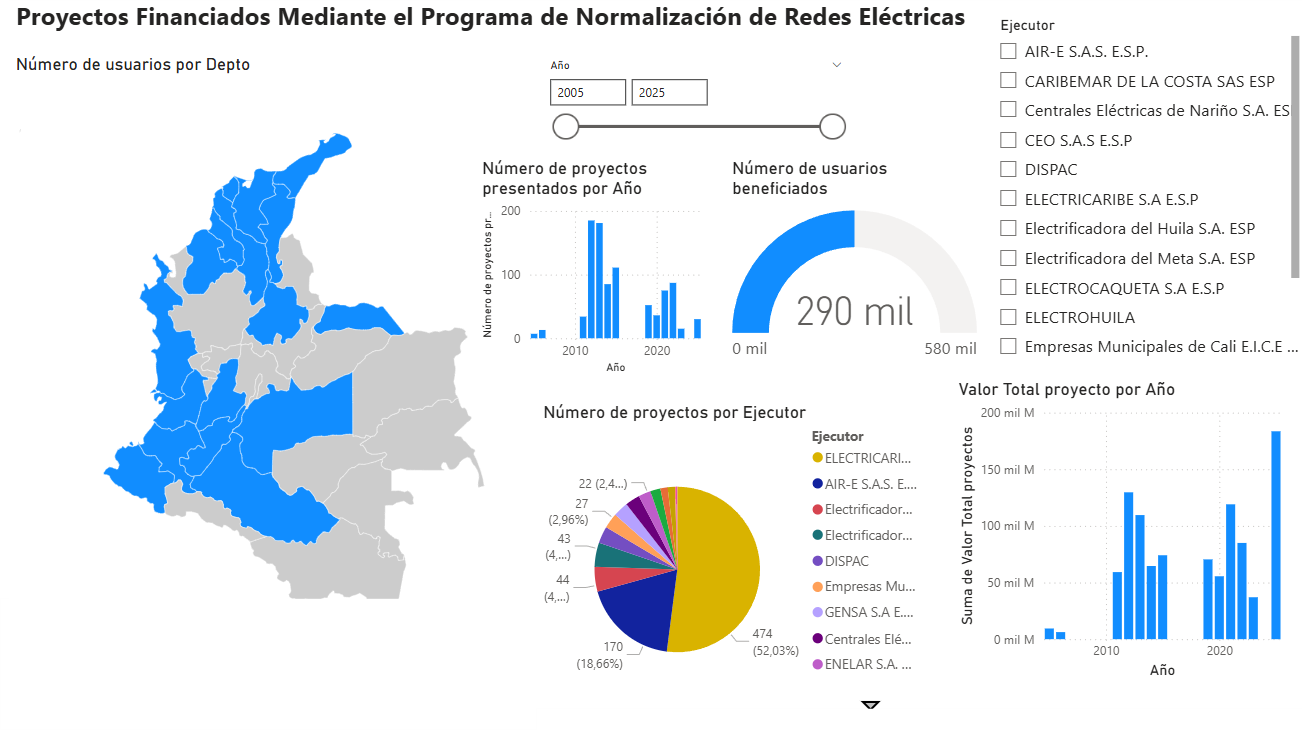
\includegraphics[width=\textwidth]{figura_prone_historico.png}
\caption{Proyectos financiados con recursos públicos, vigencias 2003--2025}
\label{fig:prone_historico}
\footnotesize\textit{Fuente: Elaboración propia con datos de \parencite{MME2025}.}
\end{figure}

La concentración geográfica es clara: región Caribe, región Pacífica y
algunos departamentos andinos dominan el mapa. El 52,03\% de los
proyectos entre 2005 y 2025 provienen de la Electrificadora de la Costa
Caribe (hoy Afinia), seguida por Air-e (Figura~\ref{fig:prone_or}).

\begin{figure}[H]
\centering
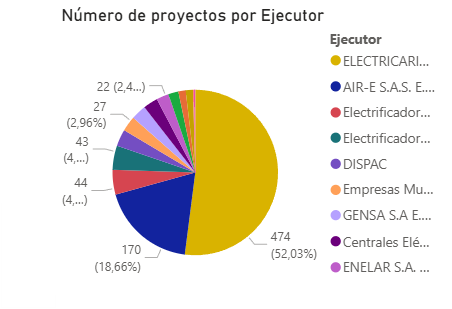
\includegraphics[width=0.72\textwidth]{figura_prone_por_or.png}
\caption{Proyectos presentados por Operador de Red, vigencias 2005--2025}
\label{fig:prone_or}
\footnotesize\textit{Fuente: Elaboración propia con datos de \parencite{MME2025}.}
\end{figure}

Esa concentración no garantiza calidad en la formulación. En 2024,
ningún proyecto de ningún OR cumplió los requisitos. El caso de CENS
ilustra el problema desde otro ángulo: ese OR no ha participado en las
convocatorias del MME porque las alcaldías de su área de cobertura no
han ejecutado las certificaciones de BS requeridas
\parencite{CabralesSanjuan2015}. La barrera no es técnica. Es
institucional.

\subsubsection{Variaciones anuales en proyectos y beneficiarios}

La Figura~\ref{fig:prone_proyectos_usuarios} muestra el número de
proyectos y usuarios beneficiados por vigencia.

\begin{figure}[H]
\centering
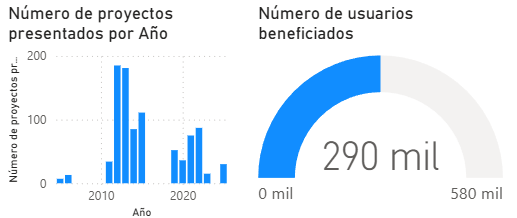
\includegraphics[width=0.90\textwidth]{figura_prone_proyectos_usuarios.png}
\caption{Proyectos presentados y usuarios beneficiados, vigencias 2005--2025}
\label{fig:prone_proyectos_usuarios}
\footnotesize\textit{Fuente: Elaboración propia con datos de \parencite{MME2025}.}
\end{figure}

Entre los periodos más relevantes se destacan los siguientes:

\textbf{2007--2010}: Sin proyectos aprobados. El ajuste normativo tras
la Ley 1117 de 2006 y el Decreto 1123 de 2008 detuvo el programa
mientras se redefinían condiciones, actores y procedimientos.

\textbf{2012}: 185 proyectos, el pico histórico del programa. Resultado
probable de años de acumulación de diagnósticos técnicos en los OR.

\textbf{2016--2018}: De nuevo sin adjudicaciones. Coincide con el ajuste
institucional del DUR 1073 de 2015.

\textbf{2024}: Cero proyectos elegibles. Primera convocatoria sin
ningún resultado. Ese dato confirma la brecha metodológica que justifica
esta monografía \parencite{MME2025}.

\textbf{2025}: 30 proyectos con el nuevo esquema AGPE, beneficiando
cerca de 11.000 usuarios en La Guajira, Magdalena, Atlántico, Nariño,
Huila y Meta.

\subsubsection{Inversión histórica por vigencia}

\begin{figure}[H]
\centering
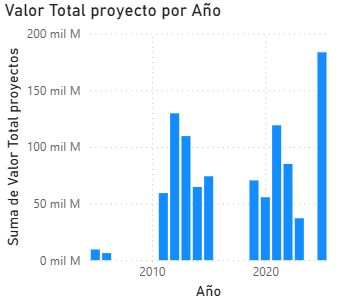
\includegraphics[width=0.65\textwidth]{figura_prone_inversion.png}
\caption{Inversión por año en proyectos de normalización, vigencias 2005--2025}
\label{fig:prone_inversion}
\footnotesize\textit{Fuente: Elaboración propia con datos de \parencite{MME2025}.}
\end{figure}

\begin{figure}[H]
\centering
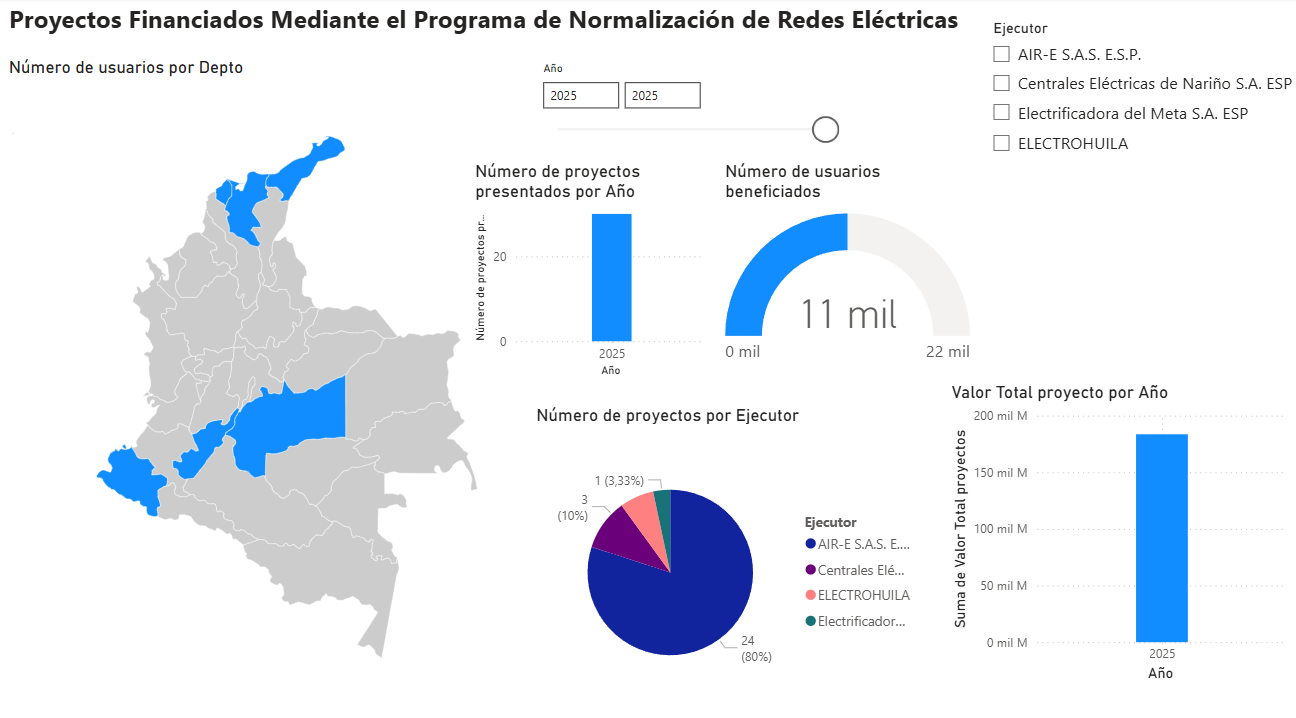
\includegraphics[width=\textwidth]{figura_prone_2025.png}
\caption{Proyectos financiados en la vigencia 2025}
\label{fig:prone_2025}
\footnotesize\textit{Fuente: Elaboración propia con datos de \parencite{MME2025}.}
\end{figure}

La vigencia 2025 es la más atípica del periodo analizado: con solo 30
proyectos —menos de una quinta parte del pico de 2012— el valor de
financiación solicitado es comparable al de vigencias con muchos más
proyectos. Eso es directamente atribuible al componente AGPE: cada
sistema fotovoltaico representa un costo adicional que eleva de manera
sustancial el costo por usuario respecto a la normalización convencional.

En total, entre 2003 y 2025 el PRONE reporta cerca de \textbf{290.000
usuarios beneficiados} según proyectos aprobados. Esa cifra puede
diferir del número real ejecutado por los ajustes que ocurren durante
la obra.


% ─────────────────────────────────────────────────────────────
\section{Análisis Técnico del Caso de Estudio}
\label{sec:caso_tecnico}
% ─────────────────────────────────────────────────────────────

Esta sección construye un caso de estudio hipotético basado en las
condiciones reales de la región Caribe para evaluar la viabilidad de
integrar AGPE en un proyecto de normalización. Los parámetros de
demanda vienen del Capítulo~\ref{chap:diagnostico} y la normativa de
referencia del Capítulo~\ref{chap:normativo}. El análisis compara los
escenarios con y sin AGPE.

\subsection{Lineamientos técnicos y sociales para la integración de sistemas AGPE en proyectos de normalización}
\label{subsec:lineamientos_agpe}

La integración de estos dos sistemas eléctricos que garanticen un beneficio real y duradero para los usuarios necesita el cumplimiento de estándares técnicos y el fortalecimiento comunitario y social en pro de la apropiación y sentido de pertenencia sobre el proyecto. A continuación se definen los lineamientos mínimos para ello.

\subsubsection{Lineamientos Técnicos}

\textbf{Articulación normativa:} El Reglamento Técnico de Instalaciones Eléctricas (RETIE) establece las condiciones mínimas que una instalación eléctrica debe cumplir, entre ellas distancias de seguridad, selección de constructores y regulación de tensión, entre otros; y la Resolución CREG 174 de 2021 constituyen la normatividad que rige el diseño, dimensionamiento y la conexión del sistema AGPE a la red de distribución. Dentro de los requisitos principales para el dimensionamiento, la Resolución 174 limita la potencia máxima instalada de un sistema AGPE al 50\% de la capacidad del transformador o circuito de conexión \parencite{ResolucionCREG174_2021}.

Adicionalmente, estipula que los excedentes que superen la importación se reconocerán a los usuarios a través de créditos de energía. Aunado a ello, establece los componentes de la tarifa que el usuario debe pagar según la capacidad del sistema AGPE ($<$ ó $>$ 100~kW): Comercialización, Distribución, Transmisión, Pérdidas Reconocidas y Restricciones. Así mismo, es pertinente recalcar que si bien ambos sistemas están integrados, el dimensionamiento de la red de distribución no está estrictamente ligado al del sistema AGPE, dado que si el sistema es de generación solar fotovoltaica su mayor producción se da en horas del día, mientras que la curva de carga muestra que el pico máximo de demanda se da en horas de la noche. En consecuencia, el diseño de la red de distribución sigue estando ligado principalmente a los picos de demanda \parencite{CREGCargoRespaldo2023, ResolucionCREG174_2021}.

\textbf{Sistema de medición inteligente:} Debido a la naturaleza del proyecto y a la exigencia en las convocatorias del MME, se requieren medidores con tecnología AMI y bidireccionales, ya que permiten identificar los excedentes entregados a la red por el sistema AGPE con el fin de ser reconocidos a los usuarios.

\textbf{Dimensionamiento del sistema de AGPE:} Con base en las dos resoluciones direccionadas al financiamiento de sistemas de normalización con AGPE, la capacidad instalada de los sistemas debe garantizar el consumo básico de subsistencia. Para ello, el cálculo de potencia debe ajustarse al factor de planta real del área de influencia.

\subsubsection{Lineamientos Sociales}

\begin{itemize}
    \item \textbf{Conformación de Comunidades Energéticas:} A través del ``Plan de Acción Social'' formulado por el MME en las convocatorias de la vigencia 2025, la organización de los usuarios bajo la figura de Comunidades Energéticas es un requisito durante la ejecución de los proyectos. Si bien no se define el prestador de servicio público responsable del AOM del sistema de AGPE, este debe plantearse teniendo en cuenta que la gestión del sistema es colectiva y es importante el fortalecimiento y apropiación de los usuarios con respecto a la infraestructura eléctrica del proyecto.

    \item \textbf{Formación y capacitación:} Conforme al Plan de Acción, este tipo de proyecto hace obligatoria la formación básica de los beneficiarios en AOM, en el uso racional y gestión eficiente de la energía. Esto engloba temas como la interpretación de los datos de un medidor y la cadena de valor. Los conocimientos adquiridos podrán romper las barreras sociales que afectan la ejecución de los proyectos de normalización en torno al aumento de la factura, mejorando los hábitos de consumo en los BS y garantizando la sostenibilidad del sistema de AGPE.
\end{itemize}


\subsection{Dimensionamiento técnico y económico de la normalización con AGPE}
\label{subsec:dimensionamiento_caso}

El dimensionamiento de la red de distribución integrada y del sistema de autogeneración se realiza teniendo en cuenta, entre otras variables, la demanda energética, la capacidad de los equipos de generación fotovoltaica y la infraestructura mínima de una red en Media Tensión (MT) y Baja Tensión (BT) requerida para garantizar el cumplimiento de la normativa vigente.

Para la selección del área de influencia, se tomaron como referencia los proyectos presentados en las convocatorias del año 2025, dado que representan el único antecedente a la fecha de proyectos de normalización adjudicados con inclusión de sistemas AGPE. De los cuatro OR que presentaron proyectos y obtuvieron concepto FAVORABLE, Air-e fue el único con presencia en la región Caribe. Teniendo en cuenta que en el Capítulo~\ref{chap:diagnostico} se determinó que esta región es la zona donde más se presenta el fenómeno de subnormalidad y que el clima cálido húmedo eleva el consumo por necesidades de confort térmico, se seleccionó el proyecto en el BS ``El Espinal''.

A continuación se describen los criterios de entrada:

\begin{itemize}
    \item \textbf{Ubicación:} municipio Malambo, Atlántico
    \item \textbf{Cantidad de usuarios:} 106
    \item \textbf{Parámetros ambientales promedio:} T~27\,°C; HR~82\%; A~10~msnm
    \item \textbf{Consumo promedio por usuario:} 235~kWh/mes
    \item \textbf{Consumo básico de subsistencia:} 173~kWh/mes
    \item \textbf{Estrato socioeconómico:} 1
    \item \textbf{Certificación:} expedida por el ente territorial como BS
    \item \textbf{Área disponible:} El polígono resaltado en rojo tiene un área de 77,72~ha, que para el caso de estudio corresponde al BS ``El Espinal''. Así mismo, la ubicación de las 106 viviendas está alrededor de la ruta marcada en amarillo, la cual tiene una longitud de 1,289~km (ver Figura~\ref{fig:delimitacion_bs}).
\end{itemize}

\begin{figure}[H]
\centering
%\includegraphics[width=0.85\textwidth]{figura_delimitacion_bs.png}
\caption{Delimitación geográfica del BS ``El Espinal''}
\label{fig:delimitacion_bs}
\footnotesize\textit{Fuente: Elaboración propia en Google Earth.}
\end{figure}


\subsection{Diseño eléctrico de la normalización de redes}
\label{subsec:disenio_electrico}

El diseño eléctrico del proyecto se desarrolla conforme a la Resolución
MME 40117 de 2024 que modificó el RETIE. La normatividad técnica de
referencia es:

\begin{itemize}
    \item RETIE -- Resolución MME 40117 de 2024.
    \item RETILAP.
    \item Normas ICONTEC.
    \item Código Eléctrico Colombiano (NTC 2050).
    \item Normas y especificaciones del OR correspondiente.
    \item Especificaciones de fabricantes de equipos y materiales.
\end{itemize}

Los ítems del diseño, conforme al RETIE, son:

\begin{enumerate}[label=\alph*), leftmargin=1.8cm, itemsep=3pt]
    \item Análisis de riesgos de origen eléctrico y medidas de mitigación.
    \item Análisis de riesgos por descargas atmosféricas y medidas de protección.
    \item Análisis y cálculo de cargas iniciales y futuras, incluyendo factor de potencia y armónicos.
    \item Coordinación de aislamiento eléctrico.
    \item Análisis y cálculo de cortocircuito, arco eléctrico y falla a tierra.
    \item Análisis del nivel de tensión requerido.
    \item Cálculos de campos electromagnéticos.
    \item Cálculo de transformadores incluyendo efectos de armónicos y factor de potencia.
    \item Sistema de puesta a tierra.
    \item Cálculo económico de conductores teniendo en cuenta factores de pérdidas y costos de la energía.
    \item Especificación de conductores conforme a IEC 60909 u equivalente.
    \item Cálculo mecánico de estructuras y elementos de sujeción de redes.
    \item Cálculo y coordinación de protecciones contra sobrecorrientes conforme a IEC 60947-2 Anexo A.
    \item Cálculos de canalizaciones, bandejas portacables y volumen de encerramientos.
    \item Cálculo de pérdidas de energía incluyendo efectos de armónicos y factor de potencia.
    \item Cálculos de regulación de tensión.
    \item Identificación de áreas clasificadas como peligrosas.
    \item Diagramas unifilares.
    \item Planos eléctricos para construcción.
    \item Especificaciones técnicas de equipos y materiales.
    \item Distancias de seguridad o servidumbre requeridas.
    \item Justificación de desviaciones técnicas cuando sea necesario.
    \item Selección, cálculo y especificación de equipos de generación convencionales y no convencionales.
\end{enumerate}


\subsection{Dimensionamiento eléctrico y económico del sistema de AGPE}
\label{subsec:dimensionamiento_agpe}

Considerando que el PRONE no especifica el tipo de generación a implementarse, sino por el contrario lo deja abierto a FNCER, fue necesario realizar un análisis de alternativas para identificar la tecnología adecuada para el caso de estudio, teniendo en cuenta el recurso energético disponible, los costos de inversión inicial, los costos fijos de operación y mantenimiento (O\&M) y la generación requerida. El proyecto debe suplir como mínimo el consumo básico de subsistencia (173~kWh/mes, según lo establecido en la Resolución 355 de 2004) de acuerdo con las Resoluciones 40243 y 40432 de 2025; por lo tanto, el sistema se dimensionará con respecto a este valor para los 106 usuarios \parencite{ResolucionCREG355_2004, ResolucionMME40243_2025, ResolucionMME40432_2025}.

Al observar la tabla comparativa de las seis tecnologías dispuestas a pequeña escala (Tabla~\ref{tab:tecnologias_fnce}), se evidencia que en Colombia la tecnología con mayor despliegue es la solar fotovoltaica. Esta opción resulta ser la más económica en términos globales y la que requiere un menor porcentaje de inversión destinado a la instalación, alineado a que requieren un menor tiempo para su construcción, permitiendo que los proyectos se ejecuten con agilidad tal que puedan estar operativos en paralelo a la normalización de las redes eléctricas. Adicionalmente, presenta una ventaja competitiva ya que el costo de O\&M es mucho menor en comparación con las demás tecnologías \parencite{UPMECatalogoTecnologico2024}.

Al analizar las demás tecnologías según sus particularidades, se evidenció que las Pequeñas Centrales Hidroeléctricas (PCH) a filo de agua se ven seriamente afectadas por el fenómeno del Niño debido a la falta de almacenamiento de agua. Por tanto, la disminución del caudal de los ríos durante estos periodos reduciría la capacidad de autogeneración precisamente cuando más se necesita, ya que es en esos instantes cuando la tarifa de energía sube en todo el territorio nacional debido a que la matriz energética depende en más de un 70\% del recurso hídrico \parencite{XMGeneracionReal2025}. Por lo tanto, la autogeneración con PCH no estaría alineada con los picos de tarifa y no atacaría el problema central: la reducción de costos para los usuarios en condiciones de subsistencia durante los meses críticos \parencite{UPMECatalogoTecnologico2024}.

En cuanto a la geotermia, la dinámica de financiación del PRONE exige que en el momento de la convocatoria el sistema ya cuente con un diseño definido. Esto implicaría que el OR debería asumir previamente los gastos de exploración, pruebas y estudios técnicos requeridos para garantizar el recurso. Como se observa en la caracterización técnica y económica, el costo de estos estudios iniciales es elevado, llegando a superar incluso la inversión total de un sistema solar completo, lo que vuelve inviable esta alternativa para un proyecto de normalización social, donde el OR busca financiamiento del Estado para solventar una problemática que afecta su cartera \parencite{UPMECatalogoTecnologico2024}.

De igual manera, la biomasa y el biogás dependen estrictamente de ciclos agrícolas, recolección de residuos y procesos de tratamiento o transporte de insumos. Al tratarse de un municipio con baja actividad económica agrícola, bovina y porcina, especialmente en el área de influencia, no se tendría garantizado el suministro constante de combustible, convirtiéndose en una carga logística y económica para los mismos usuarios \parencite{UPMECatalogoTecnologico2024}.

Finalmente, es importante considerar que todas estas tecnologías alternativas requieren un conocimiento técnico más complejo para su operación y mantenimiento. Dadas las capacidades educativas de los habitantes en estos barrios, un sistema difícil de operar generaría un cuello de botella que afectaría la infraestructura a mediano plazo, especialmente si el sistema queda a cargo de la comunidad bajo la figura de una Comunidad Energética. Por estas razones, la tecnología solar se consolida como la opción más viable, sostenible y de fácil apropiación para los usuarios, aunado a que el municipio de Malambo cuenta con una irradiancia solar en promedio entre 5,0 y 5,5~kWh/m\textsuperscript{2}/día, siendo de los mejores promedios en todo el territorio nacional \parencite{UPMECatalogoTecnologico2024}.

A continuación, en la Tabla~\ref{tab:tecnologias_fnce} se presenta cada una de las tecnologías disponibles en Colombia a pequeña escala y su caracterización técnica y económica.

\begin{table}[H]
\centering
\caption{Comparación técnica y económica de las tecnologías FNCER existentes a pequeña escala}
\label{tab:tecnologias_fnce}
\footnotesize
\begin{tabularx}{\textwidth}{>{\RaggedRight}p{2.2cm}
                             >{\RaggedRight}X
                             >{\RaggedRight}X
                             >{\RaggedRight}X
                             >{\RaggedRight}X
                             >{\RaggedRight}X
                             >{\RaggedRight\arraybackslash}X}
\toprule
\textbf{Atributo} & \textbf{Solar FV} & \textbf{Eólica terrestre} & \textbf{Filo de agua} & \textbf{Geotermia binaria} & \textbf{Biomasa} & \textbf{Biogás} \\
\midrule
\rowcolor{grisclaro}
Categoría & Cat.\ 3, en transición a Cat.\ 4 & Cat.\ 3 & Cat.\ 3 & Cat.\ 3 & Cat.\ 3 & Cat.\ 3 \\

Tamaño y capacidad & 1,5--2,1~m\textsuperscript{2}; 450--670~Wp & 1--25~kW & Hasta 1~MW & 1--10~MW & 1--60~MW & 10~kW--1~MW \\

\rowcolor{grisclaro}
Inversión [MUSD\,2024/MW] & 1,12 (0,23 instalación) & 3,4 (1,0 instalación) & 4,3 (2,86 instalación) & 6,0 (40\% instalación + 2,98 exploración) & 2,56 (35\% instalación) & 4,38 (19\% instalación) \\

O\&M [USD\,2024/MWe] & 11.000/año & 68.500/año & 94.000/año & 88.900/año & 60.700/año & 46.200/año \\

\rowcolor{grisclaro}
Vida útil [años] & 27 & 27 & 50 & 30 & 25 & 25 \\

Construcción [años] & 0,5 & 1 & 2 & 2 & 2 & 1,5 \\

\rowcolor{grisclaro}
Espacio [1000\,m\textsuperscript{2}/MWe] & 12,5 & 11 & 2,4 & 30 & 35 & 0,649 \\

Factor de planta [\%] & 20,3 & 26 & 56 & 88 & 52,6 & 8,2 \\
\bottomrule
\multicolumn{7}{l}{\footnotesize\textit{Fuente: Elaboración propia a partir de \parencite{UPMECatalogoTecnologico2024}.}}
\end{tabularx}
\end{table}

De acuerdo con lo anterior, la demanda de energía diaria a suplir por el sistema fotovoltaico debe ser de mínimo 5,76~kWh/día asumiendo un mes de 30 días. Como se debe suplir mínimo el consumo básico, se toman las condiciones críticas de disponibilidad del recurso solar; por ende, el dimensionamiento se realiza con la irradiancia solar del mes más bajo en el área de influencia.


% ─────────────────────────────────────────────────────────────
\section{Síntesis del Capítulo}
\label{sec:sintesis_cap4}
% ─────────────────────────────────────────────────────────────

El análisis histórico del PRONE entre 2005 y 2025 deja un panorama
claro: en veinte años de operación el programa ha beneficiado a cerca
de 290.000 usuarios, pero la demanda de normalización crece a un ritmo
del 26\% en cuatro años y los OR con mayor exposición a la subnormalidad
no tienen capacidad financiera para cofinanciar proyectos a escala. El
PRONE es la vía prácticamente exclusiva para financiar la normalización
en la región Caribe. El resultado de 2024 —ningún proyecto elegible—
confirma que la brecha no es de recursos sino de capacidad metodológica
para estructurar proyectos que cumplan los requisitos del MME.
% ============================================================
%  capitulo5_metodologia.tex
%  Capítulo 5: Metodología Integral para la Normalización
%              de Redes Eléctricas con AGPE en el Marco
%              del PRONE
% ============================================================

\chapter{Metodología Integral para la Normalización de Redes Eléctricas con AGPE en el Marco del PRONE}
\label{chap:metodologia}

Este capítulo es el producto central de la monografía. Todo lo que se
desarrolló en los capítulos anteriores —el diagnóstico de los BS, la
revisión normativa, los casos de estudio y el análisis técnico y
financiero— converge aquí en una propuesta metodológica concreta para
que los OR puedan formular y presentar proyectos de normalización con
AGPE que sean elegibles ante el MME.

La metodología no es un protocolo rígido. Es una hoja de ruta adaptable
que organiza los componentes técnicos, normativos, financieros, sociales
e institucionales del proceso en una secuencia lógica, con actores
definidos, entregables claros y criterios de avance entre fases.


% ─────────────────────────────────────────────────────────────
\section{Identificación de Actores y sus Roles en el Proceso}
\label{sec:actores}
% ─────────────────────────────────────────────────────────────

Normalizar un BS no es algo que un OR pueda hacer solo. Lo demostró
Popayán, que requirió la coordinación de más de diez entidades para
normalizar 41 asentamientos \parencite{SerranoRueda2019}. La
articulación de actores no es un requisito de forma: es la condición
que determina si el proyecto puede superar los bloqueos que
inevitablemente aparecen en el camino.

Los actores del proceso se agrupan en cinco categorías:

\subsection{Actores públicos nacionales}
\label{subsec:actores_nacionales}

\textbf{Ministerio de Minas y Energía (MME):} Administra el PRONE,
define los lineamientos de cada convocatoria, los requisitos de
elegibilidad y los criterios de priorización. Expide los actos
administrativos de adjudicación y supervisa la ejecución. Es el
destinatario final del expediente del proyecto.

\textbf{CAPRONE:} El comité colegiado que evalúa y aprueba los proyectos
en cada convocatoria. Sus actas son el registro oficial de lo que se
adjudica y a quién.

\textbf{CREG:} Define el marco regulatorio para la distribución y para
la integración de AGPE en el SIN, incluyendo los requisitos de conexión,
medición bidireccional y gestión de excedentes. La Resolución 174 de 2021
es la norma vigente \parencite{ResolucionCREG174_2021}.

\textbf{UPME:} Define la planeación energética nacional y publica los
datos de consumo de referencia por piso térmico. También fija los límites
de potencia para los sistemas AGPE \parencite{UPME2025}.

\textbf{SSPD:} Es la administradora del SUI, donde se centralizan los
reportes realizados por los prestadores de servicios públicos del SIN a
través de formatos previamente estructurados. Esta información no solo
permite la vigilancia de las entidades en la cadena de valor, sino que
representa el insumo para informes, estadísticas, investigaciones y
control social, entre otros. Por tanto, al ser el sistema definido para
ello, el MME se basa en el registro de los formatos S4, TC1 y TC2 para
la asignación del subsidio FOES y la habilitación de los barrios
subnormales en sus convocatorias.

\subsection{Actores territoriales}
\label{subsec:actores_territoriales}

\textbf{Alcaldías municipales y distritales:} El actor territorial más
crítico. Sin la certificación del alcalde, ningún proyecto puede
presentarse al PRONE. Punto. No importa cuánto tiempo lleve el barrio en
subnormalidad ni qué tan bien esté diseñado el proyecto técnico. Es a
través de su Plan de Ordenamiento Territorial (POT), Plan Básico de
Ordenamiento Territorial (PBOT) o Esquema de Ordenamiento Territorial
(EOT) que se reconoce legalmente la subnormalidad a través de la
certificación. Las alcaldías también son actores clave en la gestión
social previa y en la articulación con la comunidad durante las obras.
Adicionalmente, una vez las redes de los BS sean aptas, la entidad
territorial es la encargada de prestar el alumbrado público, garantizando
continuidad, calidad del servicio y los niveles de cobertura adecuados
conforme a lo estipulado en el artículo 4 del Decreto 943 de 2018
\parencite{Decreto943_2018}.

\textbf{Gobernaciones:} Pueden articular entre el nivel nacional y el
municipal, especialmente en departamentos con alta concentración de BS
y débil capacidad institucional municipal.

\subsection{Actores operativos del sector eléctrico}
\label{subsec:actores_operativos}

\textbf{Operadores de Red (OR):} Tienen la mayor responsabilidad del
proceso. Deben identificar y diagnosticar los BS en su área, gestionar
la certificación ante los entes territoriales, formular y presentar
el proyecto, contratar y supervisar las obras, y asumir la AOM de los
activos de la red una vez terminadas las obras. En proyectos con AGPE,
también asumen la responsabilidad técnica de la conexión al SIN, salvo
que los activos de generación se cedan a una Comunidad Energética
\parencite{Decreto1023_2024}.

\textbf{Comercializadores:} En los BS, el OR frecuentemente actúa
también como comercializador. Cuando opera un comercializador distinto,
se introduce una capa adicional de coordinación para el manejo de los
esquemas diferenciales de facturación.

\subsection{Actores privados de soporte}
\label{subsec:actores_privados}

\textbf{Contratistas y constructores:} Ejecutan las obras bajo
supervisión del OR. Para trabajar en BS no basta con experiencia técnica
eléctrica: los trabajadores de obra son el primer contacto visible del
proyecto con la comunidad, y eso importa.

\textbf{Proveedores de equipos:} Suministran materiales de red y equipos
del sistema AGPE. En la región Caribe, la disponibilidad local de
proveedores con garantía y postventa es un criterio de selección
relevante que no siempre se considera en la formulación.

\textbf{Firmas consultoras:} Apoyan al OR en la formulación, el diseño
técnico, el presupuesto y la preparación del expediente. Son
especialmente valiosas en los OR con menor capacidad interna de
estructuración, que son precisamente los que históricamente han tenido
más problemas para presentar proyectos elegibles.

\subsection{Actores sociales y comunitarios}
\label{subsec:actores_comunitarios}

\textbf{Juntas de Acción Comunal (JAC):} El interlocutor comunitario
más directo. Su respaldo al proceso puede ser la diferencia entre una
obra que avanza y una que la comunidad bloquea. Cuando la JAC asume el
rol de suscriptor comunitario durante la transición, esa figura debe
manejarse con cuidado: la JAC no tiene herramientas legales para exigir
el pago individual a los usuarios.

\textbf{Líderes sociales e informales:} En los BS hay liderazgos con
más influencia real que la JAC formal. Identificarlos y vincularlos
desde el inicio del proceso es una de las acciones con mayor retorno
en la gestión social.

\textbf{Comunidades Energéticas:} Figura reglamentada por el Decreto
2236 de 2023 que permite a un grupo de usuarios asumir el carácter
legal de prestador de servicio público y gestionar los activos AGPE
construidos con recursos del PRONE. La Comunidad Energética puede estar
facultada para la gestión de los activos del sistema de AGPE y para
suscribir contratos o convenios asociativos para desarrollar las
actividades de generación, comercialización, y uso eficiente de la
energía. Su constitución requiere un proceso de formación comunitaria
que debe iniciarse con suficiente anticipación a la finalización de las
obras \parencite{Decreto2236_2023}.

La Tabla~\ref{tab:actores_roles} sintetiza los actores, su fase de
intervención y su función principal.

\begin{table}[H]
\centering
\caption{Actores del proceso de normalización con AGPE, fases de intervención y función principal}
\label{tab:actores_roles}
\begin{tabularx}{\textwidth}{>{\RaggedRight}p{2.2cm}
                             >{\RaggedRight}p{3.8cm}
                             >{\RaggedRight}p{2.8cm}
                             >{\RaggedRight\arraybackslash}X}
\toprule
\textbf{Tipo} & \textbf{Entidad} & \textbf{Fase} & \textbf{Función principal} \\
\midrule
\rowcolor{grisclaro}
Públicos nacionales & MME, CAPRONE, CREG, UPME, SSPD & Planeación, regulación y aprobación & Administración del PRONE, definición de políticas y normas, aprobación de proyectos y supervisión. \\
Territoriales & Alcaldías, gobernaciones & Diagnóstico y gestión & Certificación del BS, articulación comunitaria, acompañamiento social y soporte institucional local. \\
\rowcolor{grisclaro}
Operativos & OR, comercializadores & Planeación, ejecución y operación & Diagnóstico técnico, diseño, formulación, construcción, puesta en servicio y AOM. \\
Privados de soporte & Contratistas, proveedores, consultoras & Ejecución & Materiales, mano de obra calificada y consultoría técnica. \\
\rowcolor{grisclaro}
Sociales y comunitarios & JAC, líderes sociales, Comunidades Energéticas & Diagnóstico, ejecución y seguimiento & Socialización, apropiación del proyecto, gestión comunitaria y AOM de activos AGPE. \\
\bottomrule
\multicolumn{4}{l}{\footnotesize\textit{Fuente: Elaboración propia.}}
\end{tabularx}
\end{table}


% ─────────────────────────────────────────────────────────────
\section{Requisitos para la Financiación a través del PRONE}
\label{sec:requisitos}
% ─────────────────────────────────────────────────────────────

En 2024, ningún proyecto cumplió los requisitos del PRONE
\parencite{MME2025}. Ese resultado no es anecdótico: es la señal más
clara de que muchos OR no dimensionan bien la complejidad de lo que se
les pide. Los requisitos abarcan cuatro dimensiones, y el incumplimiento
de cualquiera de ellas es causal de descalificación.

\subsection{Requisitos técnicos}
\label{subsec:req_tecnicos}

\textbf{Para la red de normalización:}
\begin{itemize}
    \item Diseño eléctrico completo conforme al RETIE (Resolución MME
    40117 de 2024), incluyendo análisis de riesgos, cálculos de carga,
    selección de conductores, coordinación de protecciones, sistema de
    puesta a tierra, diagramas unifilares y planos de construcción.
    \item Los gastos elegibles se limitan a redes de distribución,
    transformadores, acometidas y medidores. El desmonte del material
    existente no puede superar el 3\% del valor total del proyecto
    \parencite{DUR1073_2015}.
    \item Cumplimiento del Código Eléctrico Colombiano (NTC 2050) y de
    las normas técnicas del OR.
    \item Diseños de ingeniería, memorias de cálculo y planos (eléctricos
    y civiles), aportados a título gratuito al MME.
    \item Cronograma proyectado para la ejecución del proyecto y las
    actividades requeridas.
    \item Plan donde se determinen las estrategias para garantizar la
    sostenibilidad del proyecto a nivel social, ambiental y económico.
\end{itemize}

\textbf{Para el sistema AGPE:}
\begin{itemize}
    \item Potencia máxima instalada: 1~MW, conforme a la Resolución
    UPME 281 de 2015 \parencite{ResolucionUPME281_2015}.
    \item La potencia del AGPE no puede superar el 50\% de la capacidad
    del transformador o circuito al que se conecta, conforme a la
    CREG 174 de 2021 \parencite{ResolucionCREG174_2021}.
    \item Medición bidireccional obligatoria.
    \item El diseño debe incluir los estudios de recurso solar,
    dimensionamiento del sistema, verificación del límite del 50\% y
    compatibilidad con la red del OR.
    \item Si los activos se ceden a una Comunidad Energética: acto de
    constitución conforme al Decreto 2236 de 2023 y plan de AOM
    aprobado por el OR.
    \item Diagramas unifilares existentes y proyectados, incluyendo
    sistema de infraestructura de medición avanzada (AMI).
    \item Análisis de alternativas del sistema AGPE.
\end{itemize}

\subsection{Requisitos sociales}
\label{subsec:req_sociales}

Los 20 expertos consultados dieron 5 sobre 5 al acompañamiento social.
No hubo una sola excepción. Eso significa que el componente social no
es opcional en la formulación del proyecto: es parte estructural del
expediente. Los requisitos concretos son:

\begin{itemize}
    \item \textbf{Diagnóstico social previo:} Caracterización
    socioeconómica y cultural del BS, incluyendo liderazgos, historias
    previas de intervención, presencia étnica y nivel de resistencia
    esperado.

    \item \textbf{Plan de gestión social:} Documento con cronograma,
    metodología, responsables y presupuesto para las acciones de
    socialización antes, durante y después de las obras.

    \item \textbf{Acuerdo con el suscriptor comunitario o JAC} sobre el
    esquema de facturación diferencial durante la transición.

    \item \textbf{Plan de eficiencia energética:} Acciones para reducir
    el consumo de los hogares post-normalización, de manera que el
    impacto de la factura sea manejable. En proyectos con AGPE, debe
    incluir información sobre los beneficios esperados del sistema solar
    en la factura del usuario.

    \item \textbf{Posición clara sobre las deudas históricas:} La
    experiencia de Popayán es contundente — sin condonación de deudas,
    no hubo normalización sostenible \parencite{SerranoRueda2019}.
\end{itemize}

\subsection{Requisitos económicos}
\label{subsec:req_economicos}

\begin{itemize}
    \item \textbf{Presupuesto detallado:} Desagregado por componentes
    (red MT, transformadores, red BT, medidores, acometidas, AGPE,
    gestión social, interventoría), con cantidades de obra, precios
    unitarios verificables y valores totales. Incluye presupuesto y
    costos del proyecto a nivel global y unitario.

    \item \textbf{Proyecto formulado en la Metodología General Ajustada
    (MGA):} Herramienta diseñada por el DNP para la formulación y
    evaluación de proyectos de inversión pública, requerida para la
    presentación del expediente.

    \item \textbf{Plan de inversiones quinquenal:} Con recursos del OR,
    demostrando la capacidad de inversión y el compromiso financiero
    con el proyecto.

    \item \textbf{Costo por usuario:} El CAPRONE evalúa si la relación
    entre el valor del proyecto y el número de familias beneficiadas es
    coherente con el histórico del programa. La referencia disponible
    es \$1.093.052 por usuario en proyectos sin AGPE
    \parencite{CabralesSanjuan2015}, actualizable por inflación y
    complementada con el costo adicional del componente solar.

    \item \textbf{Análisis de impacto tarifario:} Estimación de la
    factura mensual esperada por usuario normalizado con y sin AGPE,
    comparada con el subsidio FOES. Debe mostrar que la tarifa
    resultante es compatible con la capacidad de pago del BS.

    \item \textbf{Proyección de recaudo:} Estimación conservadora del
    recaudo esperado en el primer, segundo y quinto año
    post-normalización, teniendo en cuenta la curva de adaptación de
    los usuarios a la facturación individual.
\end{itemize}

\subsection{Requisitos legales y administrativos}
\label{subsec:req_legales}

Son los más estrictamente verificados por el CAPRONE y los que con más
frecuencia generan descalificación:

\begin{itemize}
    \item \textbf{Certificación de BS vigente,} expedida por el alcalde
    conforme al artículo 2.2.3.1.2 del DUR 1073 de 2015, actualizada y
    referenciando con precisión el barrio objeto del proyecto
    \parencite{DUR1073_2015}.

    \item \textbf{Carta de presentación} donde se identifiquen los datos
    generales del proyecto incluyendo el recurso solicitado.

    \item \textbf{Garantía de seriedad y/o cumplimiento de la oferta,}
    conforme a lo establecido en los términos de la convocatoria.

    \item \textbf{Acuerdo OR--comercializador} si son diferentes, para
    atender usuarios y comercializar excedentes del sistema AGPE.

    \item \textbf{Certificado de registro de los BS en el SUI,} que
    acredite que los barrios objeto del proyecto se encuentran reportados
    ante la SSPD.

    \item \textbf{Carta del ente territorial comprometiéndose con el
    alumbrado público} una vez se normalicen las redes, conforme al
    Decreto 943 de 2018 \parencite{Decreto943_2018}.

    \item \textbf{Certificación de la entidad territorial} que conste que
    el barrio es BS y defina la estratificación socioeconómica aplicable.

    \item \textbf{Acreditación del OR ante el PRONE,} incluyendo la
    condición de prestador del servicio en el área del proyecto y el
    cumplimiento de sus obligaciones con el SUI.

    \item \textbf{Estudio de títulos del terreno} para verificar que no
    hay restricciones legales que impidan ejecutar las obras.

    \item \textbf{Permisos y licencias ambientales} cuando la normativa
    vigente los exija para la instalación de infraestructura de
    distribución o de generación solar.

    \item \textbf{Constitución de la Comunidad Energética} (si aplica),
    conforme al Decreto 2236 de 2023, como parte del expediente
    \parencite{Decreto2236_2023}.

    \item \textbf{Pólizas de cumplimiento} que garanticen las
    obligaciones de ejecución y entrega ante el MME.
\end{itemize}

\subsection{Requisitos adicionales de convocatorias recientes}
\label{subsec:req_adicionales}

Las convocatorias más recientes del PRONE han incorporado requisitos
adicionales que complementan las dimensiones anteriores y que deben
tenerse en cuenta en la formulación del expediente:

\begin{itemize}
    \item Suscripción del Plan de Acción de Responsabilidad Social del
    MME, que incluye las obligaciones asociadas a la conformación de
    Comunidades Energéticas cuando el proyecto incorpore AGPE.

    \item Restricción de que el costo de la interventoría no supere el
    7\% de los costos directos del proyecto.

    \item Garantizar como mínimo el consumo básico de subsistencia para
    los usuarios beneficiados.

    \item Listado de usuarios beneficiados, con identificación y
    ubicación de cada vivienda.

    \item Certificación del OR sobre contratación de al menos 50\% de
    personal local, apoyo a redes internas, punto de conexión del
    sistema AGPE y realización de socializaciones con la comunidad.

    \item Documento de cofinanciación, si aplica, indicando la fuente y
    el monto de los recursos complementarios.

    \item Declaración de cumplimiento de los profesionales responsables
    del diseño y la ejecución del proyecto.

    \item Análisis de riesgo del proyecto, que identifique las amenazas
    técnicas, sociales, ambientales y financieras y las medidas de
    mitigación correspondientes.
\end{itemize}


% ─────────────────────────────────────────────────────────────
\section{Hoja de Ruta Metodológica: Fases del Proceso}
\label{sec:hoja_de_ruta}
% ─────────────────────────────────────────────────────────────

La metodología se organiza en cuatro fases secuenciales y una fase
transversal de gestión social y comunitaria que acompaña todo el proceso.
Cada fase tiene un objetivo claro, actores responsables definidos,
entregables mínimos y un criterio de avance que determina cuándo puede
pasarse a la siguiente. No se puede saltar una fase. Intentarlo es
exactamente lo que explica por qué tantos proyectos llegan incompletos
al CAPRONE.

\begin{figure}[H]
\centering
%\includegraphics[width=\textwidth]{figura_metodologia_fases.png}
\caption{Fases de la metodología integral para normalización de redes eléctricas con AGPE en el marco del PRONE}
\label{fig:fases_metodologia}
\footnotesize\textit{Fuente: Elaboración propia.}
\end{figure}

\subsection{Fase 1 -- Diagnóstico integral del territorio}
\label{subsec:fase1}

\textbf{Objetivo:} Conocer el BS en todas sus dimensiones antes de
diseñar cualquier solución.

\textbf{Responsables:} OR (liderazgo), alcaldía (certificación y datos
territoriales), trabajo social (diagnóstico social), consultora técnica
si aplica.

\textbf{Actividades:}

\begin{enumerate}[label=\textbf{\arabic*.}, leftmargin=1.8cm, itemsep=6pt]

    \item \textbf{Verificar la certificación del BS.} Si no existe o
    está vencida, iniciar las gestiones ante la alcaldía de inmediato.
    Esta gestión puede tardar meses y debe arrancar con al menos seis
    meses de anticipación respecto a la fecha esperada de la convocatoria.

    \item \textbf{Censo de usuarios y levantamiento técnico de la red:}
    Número real de viviendas, inventario de infraestructura existente
    (postes, conductores, transformadores, macromedidores), estimación
    del consumo actual y caracterización del estado técnico de las redes
    internas.

    \item \textbf{Diagnóstico socioeconómico y cultural:} Condiciones
    de ingresos, estratificación, capacidad de pago, presencia de
    comunidades étnicas, liderazgos formales e informales, y experiencias
    previas del OR en ese territorio. Este último punto es especialmente
    importante: si el OR ya intervino antes y la comunidad quedó
    inconforme, eso define el punto de partida de la gestión social.

    \item \textbf{Recurso solar y condiciones climáticas:} Piso térmico
    del municipio conforme a la Resolución 194 de 2025 del Ministerio
    de Vivienda, datos de irradiación (GHI y HPS) del sitio desde el
    Atlas de Radiación Solar del IDEAM, NASA POWER o Global Solar Atlas,
    y consumo real de referencia a partir de la plataforma O3 de la SSPD
    \parencite{SSPD2025, UPME2025}. No usar los estándares del PIEC
    para dimensionar: como se mostró en el Capítulo~\ref{chap:diagnostico},
    el consumo real en los BS del Caribe supera esos valores entre un
    61\% y un 98\%.

    \item \textbf{Capacidad disponible en la red del OR:} Verificar que
    el circuito y el transformador más cercano al BS puedan absorber
    tanto la carga normalizada como la inyección del AGPE sin superar
    el límite del 50\% de la CREG 174 de 2021
    \parencite{ResolucionCREG174_2021}.

    \item \textbf{Revisión de convocatorias anteriores del PRONE:}
    Verificar las condiciones establecidas en convocatorias previas para
    identificar requisitos recurrentes, criterios de priorización y
    causales de descalificación que puedan anticiparse en la formulación.
\end{enumerate}

\textbf{Productos de la fase:}
\begin{itemize}
    \item Informe de diagnóstico integral del BS.
    \item Certificación de BS vigente (o constancia de gestión ante la
    alcaldía).
    \item Censo de usuarios con levantamiento técnico de la red existente.
    \item Datos de recurso solar del sitio.
    \item Informe de capacidad disponible en la red del OR.
\end{itemize}

\textbf{Criterio de avance:} Se puede pasar a la Fase 2 solo cuando
existen la certificación de BS vigente, el censo completo y los datos
de recurso solar. Sin la certificación, el proceso se detiene.

\textbf{Cuello de botella:} La certificación del BS depende de la
voluntad y los tiempos del ente territorial. Mitigación: iniciar las
gestiones seis meses antes de la convocatoria y mantener seguimiento
activo con la entidad territorial. Sin esta certificación, el proyecto
no puede avanzar a ninguna fase posterior.

\subsection{Fase 2 -- Diseño y dimensionamiento del proyecto}
\label{subsec:fase2}

\textbf{Objetivo:} Desarrollar el diseño completo de la red de
normalización y del sistema AGPE, y verificar que técnicamente son
compatibles entre sí y con la red del OR.

\textbf{Responsables:} OR (dirección técnica), contratista o consultora
de diseño, OR y CREG (verificación de capacidad de conexión).

\textbf{Actividades:}

\begin{enumerate}[label=\textbf{\arabic*.}, leftmargin=1.8cm, itemsep=6pt]

    \item \textbf{Diseño de la red eléctrica normalizada} conforme al
    RETIE, incluyendo los ítems de la Sección~\ref{subsec:disenio_electrico}.
    Se recomienda conductor concéntrico antifraude en BT, consistente
    con la experiencia documentada de ESSA en Santander
    \parencite{MendezFuentes2013}. El diseño debe cerrar con diagramas
    unifilares, planos de construcción y presupuesto de obra detallado.

    \item \textbf{Elaboración de memorias de cálculo y planos:} Diseños
    de ingeniería completos, memorias de cálculo y planos eléctricos y
    civiles, los cuales deben ser aportados a título gratuito al MME
    como parte del expediente.

    \item \textbf{Verificar la capacidad de conexión} consultando el
    micrositio de información de usuarios autogeneradores del OR (exigido
    por la CREG 174 de 2021). Confirmar que la potencia del AGPE no
    supera el 50\% de la capacidad disponible en el transformador o
    circuito \parencite{ResolucionCREG174_2021}.

    \item \textbf{Dimensionamiento del sistema AGPE} con base en el
    recurso solar del sitio, la demanda del BS normalizado y el límite
    del 50\%. Incluye selección de paneles, configuración de inversores
    (string o central) y sistema de medición bidireccional. Si el
    proyecto contempla almacenamiento, dimensionar el banco de baterías
    con la autonomía y profundidad de descarga requeridas. Debe incluirse
    el análisis de alternativas del sistema AGPE y los diagramas
    unifilares existentes y proyectados, así como el sistema de
    infraestructura de medición avanzada (AMI).

    \item \textbf{Definir quién es dueño del AGPE:} ¿El OR o la
    Comunidad Energética? Esta decisión determina la estructura legal
    del proyecto y el plan de AOM. Si se opta por la Comunidad
    Energética, iniciar su constitución conforme al Decreto 2236 de
    2023 \parencite{Decreto2236_2023}.

    \item \textbf{Plan de sostenibilidad:} Documento donde se determinen
    las estrategias para garantizar la sostenibilidad del proyecto a
    nivel social, ambiental y económico, incluyendo el plan de AOM para
    la red normalizada y el sistema AGPE.

    \item \textbf{Cronograma del proyecto:} Cronograma proyectado para
    la ejecución del proyecto y las actividades requeridas, alineado con
    los plazos de la convocatoria del PRONE.

    \item \textbf{Presupuesto integrado:} Un solo documento que
    consolide red de normalización y AGPE, con cantidades de obra,
    precios de mercado verificables y costo por usuario para los dos
    escenarios (solo red vs.\ red con AGPE). Incluye presupuesto a nivel
    global y unitario.
\end{enumerate}

\textbf{Productos de la fase:}
\begin{itemize}
    \item Diseño eléctrico completo de la red con memorias de cálculo y
    planos.
    \item Especificaciones y dimensionamiento del AGPE con análisis de
    alternativas.
    \item Verificación de capacidad de conexión.
    \item Presupuesto integrado con costo por usuario.
    \item Plan de sostenibilidad.
    \item Cronograma del proyecto.
    \item Decisión documentada sobre el modelo de propiedad de los
    activos.
\end{itemize}

\textbf{Criterio de avance:} El AGPE cumple el límite del 50\% y el
presupuesto es coherente con los rangos históricos del PRONE.

\textbf{Riesgos:} El más frecuente es que la capacidad disponible del
transformador o circuito existente no alcance para absorber la inyección
del AGPE, lo que obliga a incluir el refuerzo del punto de conexión en
el alcance — con el consiguiente aumento del presupuesto. Otro riesgo
real es que los requisitos de la convocatoria cambien entre el inicio
del diseño y la fecha de presentación: siempre revisar la resolución
vigente antes de cerrar el expediente.

\subsection{Fase 3 -- Estructuración y gestión del financiamiento}
\label{subsec:fase3}

\textbf{Objetivo:} Consolidar un expediente completo, coherente y
elegible, y presentarlo al MME dentro del plazo de la convocatoria para
su evaluación y aprobación por el CAPRONE.

\textbf{Responsables:} OR (consolidación y presentación), alcaldía
(certificación y soportes), consultora técnica (revisión de elegibilidad).

\textbf{Actividades:}

\begin{enumerate}[label=\textbf{\arabic*.}, leftmargin=1.8cm, itemsep=6pt]

    \item \textbf{Revisar la resolución de convocatoria vigente} antes
    de cerrar el expediente. Los requisitos cambian entre vigencias. La
    Resolución 40243 de 2025 introdujo cambios significativos al
    incorporar el AGPE como componente elegible
    \parencite{ResolucionMME40243_2025}.

    \item \textbf{Formular el proyecto en la MGA:} Presentar el proyecto
    en el formulario de la Metodología General Ajustada, herramienta
    diseñada por el DNP para la formulación y evaluación de proyectos
    de inversión pública.

    \item \textbf{Consolidar el expediente completo:} Integrar todos los
    documentos requeridos: certificación del BS, diagnóstico integral,
    diseño técnico completo (planos, memorias, unifilares),
    especificaciones del AGPE, verificación del límite del 50\%,
    presupuesto detallado, plan de gestión social, acuerdos comunitarios,
    análisis de impacto tarifario, plan de inversiones quinquenal,
    garantía de seriedad de la oferta, carta del ente territorial sobre
    alumbrado público, listado de usuarios beneficiados, certificaciones
    del OR y, si aplica, acto de constitución de la Comunidad Energética
    y documento de cofinanciación.

    \item \textbf{Suscribir el Plan de Acción de Responsabilidad Social}
    del MME, incluyendo las obligaciones asociadas a Comunidades
    Energéticas cuando el proyecto incorpore AGPE.

    \item \textbf{Revisión cruzada de elegibilidad:} Verificar ítem por
    ítem el cumplimiento de los requisitos de la convocatoria. Esta
    revisión es lo que en 2024 habría evitado que todos los proyectos
    presentados resultaran descalificados \parencite{MME2025}. Se
    recomienda que la haga un profesional externo al equipo formulador.

    \item \textbf{Radicar el expediente} ante el MME dentro del plazo,
    conservando la constancia del radicado.

    \item \textbf{Evaluación del CAPRONE:} Una vez radicado, el CAPRONE
    evalúa el proyecto conforme a los criterios de la convocatoria.
    Atender las solicitudes de información adicional del CAPRONE durante
    la evaluación, dentro de los plazos establecidos.
\end{enumerate}

\textbf{Productos de la fase:}
\begin{itemize}
    \item Expediente completo radicado ante el MME.
    \item Proyecto formulado en la MGA.
    \item Constancia de radicado.
    \item Plan de Acción de Responsabilidad Social suscrito.
    \item Respuestas documentadas al CAPRONE (si aplica).
\end{itemize}

\textbf{Riesgo principal:} Expedientes incompletos o con inconsistencias
entre los componentes técnico, financiero y social. Un profesional
externo con experiencia en evaluación de proyectos del PRONE que revise
el expediente antes de radicarlo puede evitar una descalificación
innecesaria.

\subsection{Fase 4 -- Ejecución, energización y sostenibilidad}
\label{subsec:fase4}

\textbf{Objetivo:} Ejecutar las obras, poner en servicio la
infraestructura y garantizar que los resultados se mantengan en el
largo plazo.

\textbf{Responsables:} OR (supervisión y AOM de la red), contratista
(obras), Comunidad Energética o OR (AOM del AGPE), alcaldía y entidades
de apoyo (seguimiento institucional).

\textbf{Actividades:}

\begin{enumerate}[label=\textbf{\arabic*.}, leftmargin=1.8cm, itemsep=6pt]

    \item \textbf{Contratar y ejecutar las obras} conforme al diseño
    aprobado. La interventoría es obligatoria y su costo no debe superar
    el 7\% de los costos directos del proyecto. Debe garantizarse la
    contratación de al menos el 50\% de personal local conforme a las
    certificaciones del OR.

    \item \textbf{Mantener activa la gestión social durante las obras.}
    El caso de Brisas del Venado documenta que la resistencia puede
    aparecer en cualquier momento de la ejecución, incluso cuando la
    socialización previa fue exitosa.

    \item \textbf{Pruebas de calidad y energización:} Verificar
    instalaciones conforme al RETIE, energizar la red y confirmar el
    correcto funcionamiento de los medidores individuales y del sistema
    de medición bidireccional del AGPE.

    \item \textbf{Puesta en operación del AGPE:} Verificar el
    funcionamiento del sistema fotovoltaico, la inyección o el
    autoconsumo (según la configuración) y la contabilización correcta
    en el medidor bidireccional. Si los activos se ceden a la Comunidad
    Energética, formalizar la entrega y capacitar a los gestores de la
    comunidad.

    \item \textbf{Apoyo a redes internas y punto de conexión AGPE:}
    Conforme a las obligaciones adquiridas por el OR, garantizar el
    apoyo a la adecuación de redes internas de los usuarios y la
    correcta habilitación del punto de conexión del sistema AGPE.

    \item \textbf{AOM de largo plazo:} El OR responde por la red de
    normalización de manera indefinida. Para el AGPE, la responsabilidad
    es del OR o de la Comunidad Energética según lo definido en la
    Fase 2. El plan de AOM debe prever inspecciones semestrales en el
    primer año, protocolo de respuesta ante fallas del inversor o los
    paneles (con directorio de proveedores con servicio técnico en la
    región), plan de limpieza de paneles — en el Caribe la salinidad
    y el polvo pueden reducir significativamente el rendimiento si no
    se limpia con regularidad — y seguimiento del recaudo con acciones
    correctivas cuando caiga por debajo de lo proyectado.

    \item \textbf{Evaluación de resultados a los 12 y 36 meses:}
    Porcentaje de recaudo, reducción de pérdidas, energía generada por
    el AGPE, reducción promedio de la factura del usuario, satisfacción
    comunitaria y número de usuarios que reincidieron en conexiones
    ilegales. Estos indicadores deben reportarse al MME conforme a las
    obligaciones de seguimiento de la resolución de adjudicación.
\end{enumerate}

\textbf{Productos de la fase:}
\begin{itemize}
    \item Acta de energización de la red y del AGPE.
    \item Acta de entrega de activos a la Comunidad Energética (si aplica).
    \item Informes de seguimiento a los 12 y 36 meses.
    \item Plan de AOM documentado y en ejecución.
\end{itemize}

\textbf{Riesgos principales:} La reincidencia en conexiones ilegales —
más frecuente en el primer año, cuando los usuarios aún están ajustando
sus hábitos de pago — y el deterioro prematuro del sistema AGPE por
falta de mantenimiento. El primero se mitiga con presencia periódica del
OR en el barrio. El segundo con un plan de AOM que tenga recursos reales
asignados, no solo intenciones.

\subsection{Fase Transversal -- Gestión social y comunitaria}
\label{subsec:fase_transversal}

\textbf{Objetivo:} Construir las condiciones sociales que hagan viable
la aceptación y la sostenibilidad del proyecto.

\textbf{Responsables:} OR (coordinación), trabajo social (implementación),
JAC y líderes comunitarios (interlocución), alcaldía y entidades de
apoyo (articulación institucional).

Esta fase no tiene un inicio y un fin discretos. Es transversal a las
cuatro fases secuenciales: empieza en el diagnóstico y no termina hasta
al menos un año después de la energización. Sus momentos más intensivos
son tres:

\textbf{Antes de las obras:}
\begin{itemize}
    \item Sesiones de socialización en lenguaje accesible: qué es la
    normalización, qué va a pasar en el barrio, cuánto va a costar el
    servicio, cómo funciona el AGPE y qué impacto tiene en la factura.
    La información clara sobre la tarifa es el factor que más reduce la
    resistencia inicial, según los 20 expertos consultados.
    \item Identificar y vincular activamente a los líderes con
    influencia real. Un líder que entiende y apoya el proyecto vale
    más que cualquier jornada de socialización masiva.
    \item Abordar explícitamente la desconfianza histórica hacia el OR.
    En algunos barrios ese trabajo toma más tiempo que la propia obra.
    \item Definir concertadamente el tratamiento de las deudas históricas.
    Sin condonación o refinanciación clara, la normalización empieza con
    una carga que muchas comunidades no van a aceptar
    \parencite{SerranoRueda2019}.
    \item Si hay AGPE y se prevé Comunidad Energética, iniciar la
    formación de la comunidad sobre sus derechos y responsabilidades
    como prestadora de servicio público.
\end{itemize}

\textbf{Durante las obras:}
\begin{itemize}
    \item Gestionar los conflictos que surjan: acceso a predios, cortes
    temporales, ruido, daños a bienes privados. Que la obra avance sin
    sorpresas para la comunidad.
    \item Capacitar a los usuarios en el uso seguro del nuevo servicio,
    lectura de la factura y acceso al subsidio FOES.
    \item Si hay Comunidad Energética, formalizar su constitución durante
    este periodo con asesoría jurídica y técnica.
\end{itemize}

\textbf{Post-normalización:}
\begin{itemize}
    \item Monitorear el recaudo durante los primeros seis meses con
    visitas a los sectores de menor pago.
    \item Ejecutar el plan de eficiencia energética: capacitación en
    uso racional y, si el presupuesto lo permite, el ``Cambiatón'' de
    luminarias que tan bien funcionó en Popayán
    \parencite{SerranoRueda2019}.
    \item Para proyectos con AGPE: capacitar en el monitoreo básico del
    sistema (limpieza de paneles, revisión visual de inversores, canales
    de reporte de fallas).
    \item Evaluaciones de satisfacción a los tres y doce meses.
\end{itemize}

\textbf{Productos de la fase transversal:}
\begin{itemize}
    \item Plan de gestión social documentado.
    \item Actas de sesiones de socialización.
    \item Acuerdo con el suscriptor comunitario o JAC.
    \item Decisión documentada sobre las deudas históricas.
    \item Acto de constitución de la Comunidad Energética (si aplica).
    \item Informes de seguimiento post-normalización.
\end{itemize}

\textbf{Riesgo principal:} La presencia de suscriptores comunitarios o
líderes con interés económico en mantener el esquema informal. Cobran
por las conexiones ilegales o administran el macromedidor y no quieren
perder esa posición. Identificarlos temprano y gestionar sus intereses
de manera explícita es clave para evitar que organicen la oposición. En
comunidades étnicas, los mecanismos de consulta y toma de decisiones
son diferentes y requieren tiempos distintos \parencite{DANE2018}.


% ─────────────────────────────────────────────────────────────
\section{Análisis de Replicabilidad y Recomendaciones}
\label{sec:replicabilidad}
% ─────────────────────────────────────────────────────────────

La metodología propuesta no fue diseñada para un solo barrio ni para
un único OR. Su valor radica en la posibilidad de ser aplicada de manera
sistemática en distintos contextos territoriales, siempre que se cumplan
las condiciones habilitantes del marco normativo y se adapten las
variables técnicas y sociales a las particularidades de cada caso. Esta
sección analiza los criterios de replicabilidad, identifica los vacíos
regulatorios que dificultan la implementación y formula recomendaciones
para superarlos.

\subsection{Criterios de replicabilidad}
\label{subsec:criterios_replicabilidad}

\textbf{Normativa transversal:} La metodología se fundamenta en
normativa de alcance nacional — el DUR 1073 de 2015, la CREG 174 de
2021, el Decreto 2236 de 2023, la Resolución 40243 de 2025, entre
otras —, lo que permite su aplicación en cualquier departamento del país
donde existan BS registrados en el SUI. No depende de normativa local
específica, aunque sí requiere la voluntad del ente territorial para
expedir la certificación del BS.

\textbf{Escalabilidad financiera:} El esquema de financiamiento a
través del PRONE es el mismo para todos los OR del SIN. Los requisitos
de elegibilidad, los criterios de priorización y los mecanismos de
asignación de recursos están definidos en las resoluciones de
convocatoria del MME y aplican de manera uniforme. Esto permite que
cualquier OR con capacidad de formulación —o que contrate esa capacidad—
pueda acceder al programa.

\textbf{Adaptabilidad técnica:} Las variables de diseño del sistema
AGPE (recurso solar, demanda, capacidad de la red) son específicas de
cada sitio, pero la secuencia metodológica para determinarlas es la
misma. Un OR en el Caribe y un OR en el Pacífico siguen la misma hoja
de ruta; lo que cambia es el resultado del dimensionamiento, no el
proceso para llegar a él.

\textbf{Componente social transferible:} Las estrategias de gestión
social —socialización, vinculación de líderes, tratamiento de deudas,
formación de Comunidades Energéticas— son aplicables en cualquier BS,
con las adaptaciones culturales necesarias. La experiencia de Popayán
\parencite{SerranoRueda2019} y los resultados de la consulta a expertos
muestran que los factores de éxito social son consistentes
independientemente de la región.

\subsection{Vacíos regulatorios identificados}
\label{subsec:vacios_regulatorios}

El análisis normativo del Capítulo~\ref{chap:normativo} y la aplicación
práctica de los requisitos del PRONE al diseño de la metodología
revelaron cuatro vacíos que hoy dificultan la implementación efectiva
del AGPE dentro del esquema del programa.

\textbf{Vacío 1 -- Sin incentivos para que la Comunidad Energética
gestione el AGPE.} El Decreto 2236 de 2023 habilita la cesión de
activos a las Comunidades Energéticas, pero no establece ningún
mecanismo de remuneración por esa responsabilidad. Pedirle a una
comunidad con capacidades técnicas y administrativas limitadas que
gestione un sistema fotovoltaico sin ningún incentivo económico es
poco realista \parencite{Decreto2236_2023}.

\textbf{Vacío 2 -- El subsidio FOES no está articulado con el AGPE.}
No existe ninguna disposición normativa que defina cómo se calcula el
FOES para usuarios normalizados que cuentan con generación solar. El
usuario reduce su consumo neto de la red, pero el subsidio se calcula
sobre el consumo total. Esa incoherencia fue señalada por el experto
E11 en la consulta: puede hacer que el impacto en la factura sea más
crítico de lo esperado.

\textbf{Vacío 3 -- Sin criterios de priorización específicos para
proyectos con AGPE.} Las convocatorias usan criterios generales para
todos los proyectos, sin reconocer que los proyectos con AGPE tienen
mayor complejidad de formulación y mayor costo unitario que los
convencionales \parencite{ResolucionMME40243_2025}.

\textbf{Vacío 4 -- El PRONE no exige demostrar sostenibilidad
post-normalización.} El programa financia la ejecución, pero no tiene
mecanismos que obliguen a los OR a demostrar que los resultados se
mantienen en el tiempo. Sin ese componente, se corre el riesgo de
financiar proyectos que funcionan bien en la foto inicial y se
deterioran en los años siguientes.

\subsection{Recomendaciones}
\label{subsec:recomendaciones}

A partir de los vacíos identificados y del análisis de replicabilidad,
se formulan las siguientes recomendaciones dirigidas a los actores del
proceso:

\begin{enumerate}[label=\textbf{\arabic*.}, leftmargin=1.8cm, itemsep=6pt]

    \item \textbf{Definir un esquema de remuneración para las Comunidades
    Energéticas.} El MME y la CREG deberían establecer un mecanismo de
    remuneración estructurado como un porcentaje de los excedentes
    entregados a la red o como reconocimiento tarifario dentro del FOES,
    de manera que la gestión del AGPE sea económicamente viable para la
    comunidad.

    \item \textbf{Articular el subsidio FOES con el AGPE.} El MME, la
    CREG y la UPME deben desarrollar una disposición que defina el
    cálculo del FOES para usuarios con AGPE, proporcional al consumo
    neto de la red, evitando que el beneficio de la generación solar se
    diluya por una formulación tarifaria incompatible.

    \item \textbf{Incluir criterios diferenciados de priorización para
    proyectos con AGPE.} En futuras resoluciones de convocatoria, se
    recomienda valorar el recurso solar disponible, el impacto en la
    factura del usuario, el potencial de reducción de pérdidas y la
    solidez del plan de AOM como criterios específicos de priorización.

    \item \textbf{Incorporar informes de impacto obligatorios
    post-normalización.} Se recomienda que el PRONE exija informes de
    seguimiento a los 24 y 48 meses de la energización, y que vincule
    el desempeño en proyectos anteriores a la elegibilidad para futuras
    convocatorias.

    \item \textbf{Fortalecer la capacidad de formulación de los OR.}
    Muchos OR con BS en su área de influencia no cuentan con la
    capacidad interna para formular proyectos que cumplan todos los
    requisitos del PRONE. Se recomienda que el MME, en articulación con
    la UPME, desarrolle programas de asistencia técnica y guías de
    formulación que reduzcan las barreras de entrada al programa.

    \item \textbf{Estandarizar los requisitos entre convocatorias.}
    La variabilidad de requisitos entre convocatorias dificulta la
    preparación anticipada de los expedientes. Establecer un núcleo
    estable de requisitos con variaciones marginales entre vigencias
    permitiría a los OR iniciar la formulación con mayor certeza.
\end{enumerate}
% ============================================================
%  capitulo6_conclusiones.tex
%  Capítulo 6: Conclusiones y Recomendaciones
% ============================================================

\chapter{Conclusiones y Recomendaciones}
\label{chap:conclusiones}

Este capítulo cierra la monografía con las conclusiones principales
organizadas en torno a los cuatro objetivos específicos y el objetivo
general, las recomendaciones dirigidas a los actores clave y las líneas
de investigación futura que este trabajo deja abiertas.


% ─────────────────────────────────────────────────────────────
\section{Conclusiones}
\label{sec:conclusiones}
% ─────────────────────────────────────────────────────────────

\subsection{Sobre el diagnóstico de los barrios subnormales}
\label{subsec:conc_diagnostico}

La magnitud del problema de la subnormalidad eléctrica en Colombia es
mayor de lo que indican los indicadores de cobertura convencionales. Con
más de 314.000 familias en esa condición, el 90\% concentradas en la
región Caribe, y un crecimiento del 26\% en las viviendas sin título
entre 2020 y 2024, la brecha entre la demanda de normalización y los
recursos disponibles del PRONE se amplía año tras año
\parencite{SSPD2020, DANE2024a}.

Un hallazgo que tiene consecuencias técnicas directas: los usuarios de
BS en pisos térmicos cálidos consumen entre el 61\% y el 98\% más de lo
que proyectan los estándares del PIEC \parencite{SSPD2025, UPME2025}.
Diseñar un sistema AGPE con los valores del PIEC en lugar de los datos
reales de la plataforma O3 significa subdimensionarlo, y un sistema
subdimensionado no genera el ahorro en factura que se le promete al
usuario.

La consulta a 20 expertos fue igualmente contundente: el principal
obstáculo para la normalización no es técnico. Es el miedo al incremento
de la factura y la desconfianza acumulada hacia el OR. Esos dos factores
solos explican la mayoría de los proyectos cancelados, bloqueados o
revertidos en el país, y ninguno de los dos se resuelve desde la
ingeniería. Los 20 expertos calificaron el acompañamiento social con
5 sobre 5, sin excepción.

\subsection{Sobre el marco normativo y los casos de estudio}
\label{subsec:conc_normativo}

Entre 2014 y 2025, la regulación colombiana pasó de prohibir
prácticamente la autogeneración a habilitarla dentro de los proyectos
de normalización financiados con recursos públicos del PRONE, contemplar
la cesión de activos a Comunidades Energéticas y permitir la entrega
de excedentes al SIN bajo la CREG 174 de 2021
\parencite{Ley1715_2014, Decreto1023_2024, ResolucionCREG174_2021}.
Es un cambio normativo estructural.

El problema es que ese cambio llegó sin los instrumentos metodológicos
que los OR necesitan para aprovecharlo. La vigencia 2024 lo dejó claro
de la manera más directa posible: ningún proyecto elegible. La norma
existe; la capacidad de implementación no ha madurado al mismo ritmo.

Los tres casos de estudio analizados llevan a la misma conclusión,
independientemente del OR, el periodo o la región: la calidad técnica
de la infraestructura es necesaria, pero no es suficiente. La gestión
social previa, la articulación interinstitucional y la condonación de
las deudas históricas pesan igual o más sobre los resultados a largo
plazo \parencite{CastilloQuintana1991, MendezFuentes2013,
SerranoRueda2019}.

\subsection{Sobre el análisis técnico y financiero}
\label{subsec:conc_tecnico}

Garantizar el consumo básico de subsistencia se ve limitado por la
potencia máxima que puede declarar un sistema AGPE según la normatividad
vigente, especialmente cuando su ubicación se requiere en el sitio de
consumo. Esto se debe a dos factores: primero, si el sistema es conectado
en los transformadores de BT dimensionados en la normalización, no se
puede garantizar la generación para todos los usuarios atendidos en ese
punto; y segundo, si se optara por la tipología tipo granja, la
disponibilidad del terreno se convierte en un cuello de botella porque
los usuarios del BS difícilmente cuentan con terrenos aptos para ello.

Dadas las limitaciones de potencia disponible en los puntos de conexión
y espacio en los sitios de consumo, se propone la autogeneración remota
como la alternativa técnica más viable. No obstante, esto requiere
articulación institucional con el sector público o privado, en el
entendido de que los terrenos tendrían que ser aportados al Estado por la
persona natural o jurídica que pretenda darlos en uso y goce del
proyecto, mínimo hasta la finalización de su vida útil. En las
observaciones realizadas por la ciudadanía al proyecto de resolución de
la convocatoria 001, se evidencia que otra de las alternativas viables
para garantizar este consumo básico es a través de sistemas
individuales; sin embargo, hasta la fecha en las convocatorias se ha
limitado esta tipología.

Para que el esquema de sostenibilidad sea eficiente cuando el AOM lo
pretenda asumir una Comunidad Energética, el análisis de alternativas
debe tener en cuenta que la tecnología seleccionada sea lo menos
compleja posible para que la población pueda participar en su
mantenimiento preventivo, sin que este sea el factor preponderante
frente al potencial energético, el LCOE o la afectación ambiental.

Se observó que para garantizar la sostenibilidad del sistema de AGPE se
debe lograr mínimo una generación de 153~kWh/mes por usuario, ya que
como se evidenció, si este valor es inferior el usuario seguirá viendo
una reducción en la tarifa, pero asociada al esquema de subsidios
creados en la Ley 142 \parencite{Ley142_1994}.

La viabilidad de los proyectos de normalización con AGPE en la región
Caribe no es uniforme: depende de la combinación específica de
condiciones de cada barrio, incluyendo el recurso solar disponible,
la capacidad del transformador más cercano, el número de usuarios y su
consumo real. Estos resultados confirman que la integración de AGPE en
proyectos de normalización requiere un análisis caso a caso, lo que
fundamenta los criterios técnicos y financieros incorporados en las
Fases 2 y 3 de la metodología propuesta.

\subsection{Sobre la metodología propuesta}
\label{subsec:conc_metodologia}

La metodología en cuatro fases secuenciales y una transversal propuesta
en el Capítulo~\ref{chap:metodologia} es la primera herramienta de este
tipo desarrollada en Colombia que articula de manera explícita los
componentes técnicos, normativos, financieros, sociales e
institucionales de los proyectos de normalización con AGPE dentro del
marco del PRONE. Su estructura responde directamente a la brecha que
explica por qué ningún proyecto fue elegible en 2024.

Su mayor aportación no está en el diseño eléctrico — eso está bien
cubierto por el RETIE y los estándares de los OR — sino en la
articulación de los componentes que históricamente han determinado la
diferencia entre el éxito y el fracaso: la gestión social, la
certificación de los BS, la coordinación interinstitucional y la
sostenibilidad de los activos en el largo plazo.

La fase transversal de gestión social y comunitaria es la más crítica.
Los 20 expertos, la literatura y los tres casos de estudio coinciden
en eso. Un proceso de gestión social serio no cabe en una jornada de
información de una hora antes de arrancar las obras. Requiere comenzar
con el diagnóstico del territorio, intensificarse durante las obras y
continuar activo durante al menos el primer año post-normalización. El
presupuesto del proyecto tiene que reflejarlo.

Los proyectos con incidencia directa sobre los usuarios residenciales
de estratos bajos, que están relacionados con la prestación de servicios
públicos domiciliarios y que podrían generar una modificación en la
facturación manejada históricamente, requieren un acompañamiento social
fuerte que garantice el éxito y el funcionamiento a lo largo de la vida
útil de la infraestructura. Así mismo, requieren la articulación con
entidades externas a los prestadores de servicio y del Estado.

Los sistemas de medición individuales y las funcionalidades de la
medición avanzada, entre ellas la prepago, no solo permiten mejorar la
gestión del consumo de energía, sino que tienen una connotación social
ya que inciden en la percepción del usuario sobre los hábitos de consumo
y el uso eficiente y gestión de la energía.

La región Caribe es crítica en los procesos de normalización,
independientemente de si es el Estado o el OR quien aborda la
problemática. Primero, porque es el área donde más se presenta este
fenómeno, y segundo porque el consumo energético es más elevado, sumado
a las condiciones de pobreza y bajo nivel educativo.


% ─────────────────────────────────────────────────────────────
\section{Recomendaciones}
\label{sec:recomendaciones}
% ─────────────────────────────────────────────────────────────

\subsection{Para el Ministerio de Minas y Energía}
\label{subsec:rec_mme}

\begin{enumerate}[label=\textbf{\arabic*.}, leftmargin=1.8cm, itemsep=8pt]

    \item \textbf{Publicar una guía metodológica oficial para la
    formulación de proyectos PRONE con AGPE.} El cero proyectos elegibles
    de 2024 confirma que la necesidad es real. El MME podría adoptar
    o adaptar la metodología propuesta en esta investigación como
    herramienta de soporte para los OR.

    \item \textbf{Incorporar criterios de priorización específicos para
    proyectos con AGPE.} Las convocatorias actuales aplican criterios
    genéricos que no reconocen la mayor complejidad y el mayor costo
    unitario de estos proyectos. Los criterios diferenciados deberían
    valorar el recurso solar disponible, el impacto esperado en la
    factura del usuario, la solidez del plan de AOM y la constitución
    de la Comunidad Energética.

    \item \textbf{Establecer seguimiento plurianual obligatorio.} Exigir
    informes de impacto a los 24 y 48 meses de la energización, con
    indicadores de recaudo, calidad del servicio, estado del AGPE y
    satisfacción comunitaria. Vincular el desempeño en proyectos
    anteriores a la elegibilidad para convocatorias futuras.

    \item \textbf{Definir un esquema de remuneración para las Comunidades
    Energéticas.} En coordinación con la CREG, crear un mecanismo que
    retribuya a la comunidad por la gestión de los activos AGPE cedidos
    con recursos del PRONE, haciendo esa responsabilidad económicamente
    sostenible.

    \item \textbf{Incluir como variable de priorización la socialización
    previa con la comunidad.} Se recomienda que una de las variables de
    priorización sea un documento remitido por el OR donde se evidencie
    que las comunidades beneficiarias conocen de qué trata el proyecto y
    el impacto tarifario que esto conlleva.

    \item \textbf{No exigir la inclusión obligatoria de AGPE en pisos
    térmicos templado y frío.} Se recomienda que en los pisos térmicos
    templado y frío no sea de obligatoria inclusión los sistemas de AGPE
    en los proyectos que presenten los OR en esas áreas de influencia,
    dada la menor disponibilidad del recurso solar.
\end{enumerate}

\subsection{Para los Operadores de Red}
\label{subsec:rec_or}

\begin{enumerate}[label=\textbf{\arabic*.}, leftmargin=1.8cm, itemsep=8pt]

    \item \textbf{Iniciar la gestión de certificaciones con seis meses
    de anticipación.} Sin la certificación del alcalde, no hay proyecto.
    Ese trámite puede tardar meses y depende de voluntad institucional
    que el OR no controla. Empezar tarde es el error más común y el
    más evitable.

    \item \textbf{Construir capacidad interna de formulación.} La brecha
    de 2024 no se resuelve solo contratando consultores. Los equipos del
    OR necesitan entender los requisitos del programa y poder estructurar
    proyectos elegibles con sus propios recursos. Eso requiere equipos
    multidisciplinarios que combinen ingeniería eléctrica, trabajo social
    y gestión financiera.

    \item \textbf{Presupuestar la gestión social en serio.} La experiencia
    de Popayán muestra que ese componente representa una fracción
    significativa del costo total. Tratarlo como gasto accesorio a
    minimizar es una de las razones por las que los proyectos bien
    diseñados técnicamente terminan fracasando en campo.

    \item \textbf{Mostrar la factura post-normalización desde la primera
    jornada de socialización.} Con números reales, con y sin AGPE,
    explicando el subsidio FOES. La incertidumbre sobre cuánto va a
    costar el servicio es el principal generador de resistencia
    comunitaria, y la mejor forma de reducirla es con información
    transparente desde el inicio.

    \item \textbf{Garantizar la concordancia de los documentos
    presentados en las convocatorias.} Se evidenció en las evaluaciones
    publicadas por el MME que se presentaban muchos errores de
    digitación, información incompleta, modificación de los formatos
    exigidos por la entidad, doble contabilidad en los presupuestos,
    inconsistencias en la cantidad de usuarios respecto a la
    certificación de la alcaldía y esquemas de sostenibilidad mal
    planteados.

    \item \textbf{Realizar socializaciones y capacitaciones con la
    comunidad en el primer año posterior a las obras.} Los OR, el MME
    y los entes territoriales deben reforzar la orientación en temas
    como medidas de eficiencia pasivas y activas, uso y gestión eficiente
    de la energía, cadena de valor, costo de la energía según la hora de
    consumo, interpretación de los datos del medidor, esquema de
    subsidios, entre otros.
\end{enumerate}

\subsection{Para las Alcaldías Municipales}
\label{subsec:rec_alcaldias}

\begin{enumerate}[label=\textbf{\arabic*.}, leftmargin=1.8cm, itemsep=8pt]

    \item \textbf{Mantener actualizadas las certificaciones de BS.} Es
    una obligación legal, pero también es la condición que permite a las
    familias acceder al subsidio FOES al que tienen derecho. No
    actualizarlas tiene un costo real sobre las comunidades más
    vulnerables del municipio.

    \item \textbf{Participar activamente en la gestión social de los
    proyectos.} La alcaldía no es un actor que solo firma papeles. Su
    presencia en las jornadas de socialización, su capacidad de gestión
    de conflictos comunitarios y su articulación con otras entidades del
    Estado fueron factores determinantes en Popayán
    \parencite{SerranoRueda2019}. Sin esa participación, los proyectos
    más complejos no se pueden sostener.
\end{enumerate}


% ─────────────────────────────────────────────────────────────
\section{Propuestas de Investigación Futura}
\label{sec:investigacion_futura}
% ─────────────────────────────────────────────────────────────

Este trabajo deja abiertas las siguientes líneas de investigación que
complementarían sus resultados:

\textbf{1. Distribución de pérdidas por nivel de tensión en BS de la
región Caribe.} La regulación vigente no desagrega con precisión las
pérdidas técnicas y no técnicas por nivel de tensión dentro de los BS.
Un estudio que desarrolle esa desagregación permitiría intervenciones
más focalizadas y mejores criterios de priorización del PRONE.

\textbf{2. Impacto de las Comunidades Energéticas en la sostenibilidad
del AGPE.} El Decreto 2236 de 2023 es reciente y no hay experiencias
documentadas de su aplicación en BS colombianos. Un seguimiento de tres
años a la constitución, operación y mantenimiento de una Comunidad
Energética en un BS normalizado generaría información de alto valor para
perfeccionar la regulación y los mecanismos de soporte.

\textbf{3. Interacción entre subsidios energéticos y AGPE en comunidades
de bajos ingresos.} No existe hoy ninguna disposición que articule el
FOES con la generación solar de los usuarios de BS. Un modelo que
evalúe el efecto de distintos esquemas de subsidio sobre la factura de
usuarios normalizados con AGPE podría fundamentar recomendaciones
concretas de política para el MME y la CREG.

\textbf{4. Modelo de optimización para priorizar BS a normalizar con
AGPE.} Los recursos del PRONE son limitados y la demanda supera la
capacidad de intervención. Un modelo que combine variables técnicas
(recurso solar, estado de la red, número de usuarios), sociales
(pobreza, capacidad de pago, presencia étnica) y financieras (costo
por usuario, recaudo proyectado) para priorizar los BS con mayor
potencial de impacto y sostenibilidad sería una herramienta directamente
útil para el CAPRONE.

\textbf{5. Modificación de los esquemas de subsidios existentes.} Se
propone analizar la posibilidad de que los esquemas de subsidios
tengan en cuenta la inversión realizada por el Estado a través de
proyectos financiados por fondos y programas, incluido el PRONE.

\textbf{6. Remuneración vía tarifa para el AOM de sistemas AGPE.}
Se requieren propuestas en torno a la remuneración vía tarifa para los
prestadores de servicio público que realicen la actividad de AOM de los
sistemas de AGPE financiados con recursos públicos y privados, ya que
actualmente no se encuentra regulado por la CREG.

\textbf{7. Regulación de la autogeneración remota.} Análisis y posible
modificación sobre el Proyecto de Resolución 701\_92 de 2025 expedido
por la CREG, relacionada con la regulación de los sistemas de
autogeneración remota.

\textbf{8. Plan de Normalización de Redes Eléctricas a nivel nacional.}
Si bien actualmente el MME cuenta con el Plan Nacional de
Electrificación Rural que asocia acciones sobre el PRONE, y la UPME
realiza Planes Indicativos de Expansión de la Cobertura, no está claro
cómo se aborda integralmente la subnormalidad. Dado que este es un
fenómeno que, por las condiciones socioeconómicas del país, el
crecimiento poblacional y los conflictos armados, no se va a reducir si
no se realiza una intervención planificada y focalizada.

% ── Referencias ─────────────────────────────────────────────
\printbibliography[heading=bibintoc, title={Referencias Bibliográficas}]

% ── Anexos ──────────────────────────────────────────────────
\begin{appendices}
% ============================================================
%  anexos.tex — Anexos del documento
% ============================================================

\chapter{Encuesta de Perspectiva sobre la Normalización de Redes Eléctricas en un Contexto Técnico y Social}
\label{anx:encuesta}

La encuesta se realizó mediante un formulario digital asincrónico (Google Forms) con el fin de facilitar la recolección de información, considerando la disponibilidad de los profesionales y su residencia en distintas ciudades del territorio nacional. El objetivo fue identificar la efectividad y el impacto en los OR y en los usuarios de la implementación de proyectos de normalización, y recopilar, a partir de las experiencias de los participantes, información sobre los cuellos de botella que fundamentan la necesidad de acciones complementarias en la intervención en BS.

% ── Ficha técnica ──────────────────────────────────────────

\section*{Ficha Técnica del Instrumento}
\addcontentsline{toc}{section}{A1. Ficha técnica del instrumento}

\begin{table}[H]
\centering
\caption{Ficha técnica del instrumento aplicado a expertos con experiencia en el sector eléctrico}
\label{tab:ficha_tecnica}
\begin{tabularx}{\textwidth}{>{\bfseries\RaggedRight}p{4cm} >{\RaggedRight\arraybackslash}X}
\toprule
\textbf{Atributo} & \textbf{Detalle} \\
\midrule
\rowcolor{grisclaro}
Tipo de instrumento & Encuesta con preguntas de escala Likert y de respuesta abierta, de respuesta obligatoria. \\
Medio de aplicación & Formulario asincrónico en línea (Google Forms). \\
\rowcolor{grisclaro}
Cantidad de preguntas & 17 preguntas, identificadas como P1 a P17 en el desarrollo del texto. \\
Población objetivo & Profesionales en ingeniería eléctrica, ingeniería civil, ciencias sociales y administración pública con experiencia en proyectos de normalización de redes eléctricas en Colombia. \\
\rowcolor{grisclaro}
Tamaño de la muestra & 20 expertos, identificados como E1 a E20 en el análisis de resultados. \\
Año de aplicación & 2025. \\
\rowcolor{grisclaro}
Tratamiento de datos & Anonimato garantizado, dado que el instrumento se aplica con fines estrictamente académicos. \\
\bottomrule
\multicolumn{2}{l}{\footnotesize\textit{Fuente: Elaboración propia.}}
\end{tabularx}
\end{table}

% ── Perfil de expertos ─────────────────────────────────────

\section*{Caracterización de la Experiencia de los Expertos Encuestados}
\addcontentsline{toc}{section}{A2. Caracterización de los expertos}

\begin{longtable}{>{\centering}p{1cm}
                  >{\RaggedRight}p{2.4cm}
                  >{\centering}p{1.5cm}
                  >{\RaggedRight}p{3.0cm}
                  >{\RaggedRight}p{2.8cm}
                  >{\RaggedRight\arraybackslash}p{2.5cm}}
\caption{Caracterización de la experiencia de los expertos encuestados}
\label{tab:perfil_expertos} \\
\toprule
\textbf{No.} & \textbf{Área de formación [P2]} & \textbf{Años de exp. [P3]} & \textbf{Área de desempeño [P4]} & \textbf{Región [P5]} & \textbf{Tipo de entidad [P6]} \\
\midrule
\endfirsthead
\multicolumn{6}{c}{\small(Continuación Tabla \ref{tab:perfil_expertos})} \\
\toprule
\textbf{No.} & \textbf{Área de formación [P2]} & \textbf{Años de exp. [P3]} & \textbf{Área de desempeño [P4]} & \textbf{Región [P5]} & \textbf{Tipo de entidad [P6]} \\
\midrule
\endhead
\bottomrule
\endfoot
\bottomrule
\endlastfoot

E1  & Administrador Público     & 1--2 & Técnica/Ingeniería          & Caribe                         & Público \\
\rowcolor{grisclaro}
E2  & Administrador Público     & 3--5 & Jurídica/Administrativa     & Caribe                         & Público \\
E3  & Ciencias sociales y humanas & 1--2 & Social/Comunitaria        & Caribe, Andina                 & Público \\
\rowcolor{grisclaro}
E4  & Ciencias sociales y humanas & 3--5 & Social/Comunitaria        & Caribe, Pacífico               & Público \\
E5  & Ingeniero civil           & 6--8 & Técnica/Ingeniería          & Pacífico                       & Público y privado (mayor exp. privado) \\
\rowcolor{grisclaro}
E6  & Ingeniero Eléctrico       & 1--2 & Jurídica/Administrativa     & Caribe, Pacífico, Andina, Orinoquía, Amazonía & Público \\
E7  & Ingeniero Eléctrico       & 1--2 & Técnica/Ingeniería          & Caribe, Andina                 & Público \\
\rowcolor{grisclaro}
E8  & Ingeniero Eléctrico       & 1--2 & Técnica/Ingeniería          & Caribe, Pacífico               & Público \\
E9  & Ingeniero Eléctrico       & 1--2 & Técnica/Ingeniería          & Caribe, Andina                 & Público y privado (mayor exp. privado) \\
\rowcolor{grisclaro}
E10 & Ingeniero Eléctrico       & 1--2 & Técnica/Ingeniería          & Caribe, Pacífico, Andina, Orinoquía & Público \\
E11 & Ingeniero Eléctrico       & 3--5 & Técnica/Ingeniería          & Caribe, Pacífico, Amazonas     & Público \\
\rowcolor{grisclaro}
E12 & Ingeniero Eléctrico       & 3--5 & Comercial/Pérdidas de energía & Caribe, Andina               & Público y privado (mayor exp. privado) \\
E13 & Ingeniero Eléctrico       & 3--5 & Técnica/Ingeniería          & Andina                         & Público y privado (mayor exp. público) \\
\rowcolor{grisclaro}
E14 & Ingeniero Eléctrico       & 6--8 & Técnica/Ingeniería          & Caribe, Orinoquía              & Público \\
E15 & Ingeniero Eléctrico       & 6--8 & Técnica/Ingeniería          & Caribe                         & Público \\
\rowcolor{grisclaro}
E16 & Ingeniero Eléctrico       & 6--8 & Técnica/Ingeniería          & Caribe, Pacífico               & Público \\
E17 & Ingeniero Eléctrico       & $>$9 & Comercial/Pérdidas de energía & Andina                       & Público y privado (mayor exp. público) \\
\rowcolor{grisclaro}
E18 & Ingeniero Eléctrico       & $>$9 & Técnica/Ingeniería          & Caribe, Andina                 & Público y privado (mayor exp. público) \\
E19 & Ingeniero Eléctrico       & $>$9 & Técnica/Ingeniería          & Caribe, Andina                 & Público y privado (mayor exp. público) \\
\rowcolor{grisclaro}
E20 & Ingeniero Eléctrico       & $>$9 & Técnica/Ingeniería          & Caribe                         & Público y privado (mayor exp. público) \\
\end{longtable}
\textit{Fuente: Elaboración propia.}

% ── Tabla 7: Impacto en la red ─────────────────────────────

\section*{Resultados: Impacto en la Red Eléctrica y Percepción de los Usuarios}
\addcontentsline{toc}{section}{A3. Resultados -- impacto en la red y percepción}

\begin{longtable}{>{\centering}p{0.7cm}
                  >{\centering}p{1.1cm}
                  >{\centering}p{1.1cm}
                  >{\RaggedRight}p{5.2cm}
                  >{\RaggedRight\arraybackslash}p{5.2cm}}
\caption{Importancia e impacto en la red eléctrica y en la prestación del servicio de energía de los proyectos de normalización}
\label{tab:encuesta_red} \\
\toprule
\textbf{No.} &
\textbf{Reducción PT [P7]} &
\textbf{Disminución fallas [P9]} &
\textbf{¿Considera importante la normalización para reducir accidentes eléctricos? Explique [P10]} &
\textbf{¿Cómo perciben los usuarios el cambio en la calidad y confiabilidad del servicio? [P11]} \\
\midrule
\endfirsthead
\multicolumn{5}{c}{\small(Continuación Tabla \ref{tab:encuesta_red})} \\
\toprule
\textbf{No.} & \textbf{P7} & \textbf{P9} & \textbf{P10} & \textbf{P11} \\
\midrule
\endhead
\bottomrule
\endfoot
\bottomrule
\endlastfoot

E1  & 2 & No se conoce & Sí, para evitar incendios o riesgos eléctricos. & Agradecen tener el servicio de energía pero no quieren pagar por él. \\
\rowcolor{grisclaro}
E2  & 2 & No se conoce & Sí, porque hay una gestión e intervención adecuada de las redes eléctricas. & Satisfacción asociada a la estabilidad y confiabilidad del servicio público. \\
E3  & 2 & No se conoce & Sí. La mejora de las condiciones físicas reduce las posibilidades del uso informal del servicio. Con una socialización y capacitación adecuadas, se puede sensibilizar frente a los riesgos a la vida. & Lo perciben inicialmente a través de la reducción o nulos cortes no programados y el no daño de sus electrodomésticos. Sobre la confiabilidad, las comunidades suelen desconocer su significado técnico y lo asocian con la veracidad en el cobro. \\
\rowcolor{grisclaro}
E4  & 3 & Sí & Sí, cuando se da el manejo de redes por personal no cualificado, suelen ocurrir incidentes que ponen en riesgo a la comunidad. & Usualmente es positivo, en cuanto la normalización supere la media y se den las inversiones correspondientes. Si no agrupa a la mayoría, los usuarios manifiestan malestar porque la calidad no mejora considerablemente. \\
E5  & 5 & Sí & Sí, porque la normalización reemplaza instalaciones informales o en mal estado por infraestructura técnica segura conforme al RETIE, reduciendo riesgos de cortocircuitos, sobrecargas, electrocución e incendios. & En general perciben mejora: mayor continuidad, reducción de interrupciones, estabilidad en el voltaje. Sin embargo, el cambio puede requerir adaptación porque no siempre proviene de comunidades con cultura de pago. \\
\rowcolor{grisclaro}
E6  & 3 & No se conoce & Sí. & No sé. \\
E7  & 4 & No se conoce & Sí, ya que al normalizar las redes se busca transformar las derivaciones ilícitas en conexiones que cumplan los criterios normativos de seguridad, reduciendo la posibilidad de incidentes eléctricos. & Sin información. \\
\rowcolor{grisclaro}
E8  & 4 & No se conoce & Sí. El hecho de tener una red normalizada disminuye el riesgo de instalaciones sin protecciones ni manejo correcto de cargas que puedan afectar directamente a los usuarios. & No poseo información de primera mano. \\
E9  & 4 & No se conoce & Sí, la consideraría muy importante. Una red normalizada es más fácil de inspeccionar, mantener y ampliar sin improvisación, lo que baja el riesgo de accidentes a largo plazo. & Normalmente perciben la mejora cuando disminuyen los cortes y las fluctuaciones que afectan sus electrodomésticos. Pero también puede haber percepción negativa si los eventos siguen siendo frecuentes, incluso si hay mejoras técnicas no evidentes para el usuario. \\
\rowcolor{grisclaro}
E10 & 5 & No se conoce & Sí, ya que la normalización garantiza que las instalaciones cumplan con los estándares técnicos del RETIE. & Los usuarios perciben la normalización positivamente: mayor continuidad en el servicio y menos interrupciones. \\
E11 & 2 & No & Sí, aunque debe considerarse la cantidad de usuarios normalizados que reinciden en la subnormalidad con el fin de no pagar. Las condiciones de normalidad aportan mayor seguridad, pero no garantizan que así se mantengan las redes. & Creen que lo perciben con un servicio más confiable y mejor funcionamiento de sus electrodomésticos. \\
\rowcolor{grisclaro}
E12 & 3 & No & Considero que estos barrios, dependiendo del número de habitantes, no representan una carga significativa para el sistema eléctrico por sus bajos consumos. Sí se identificaron riesgos importantes entre quienes se conectaban fraudulentamente. & En muchos casos se les cobra entre \$400.000 y más por medidores, sellos y costos de conexión. Si a esto se suma el CNR, muchas familias prefieren no conectarse porque no tienen recursos para asumir esos costos iniciales. \\
E13 & 4 & Sí & Sí, ya que medidas comunitarias pueden conllevar malas conexiones y conexiones fraudulentas que generen siniestros. & De mejor manera, ya que la acometida es específica para cada usuario. \\
\rowcolor{grisclaro}
E14 & 1 & Sí & Sí, aunque se deberían revisar los datos de la Superservicios. & La calidad y confiabilidad aumenta a pesar de la falta de percepción por parte del usuario. \\
E15 & 4 & No se conoce & Sí, debemos adecuarnos al reglamento y las normas técnicas. & Considero que hay un problema social o una cultura del no pago, y allí radican los problemas de los barrios subnormales. \\
\rowcolor{grisclaro}
E16 & 5 & Sí & Sí, la normalización es clave para reducir diferentes tipos de riesgos asociados a la prestación del servicio, ya que elimina conexiones inseguras, garantiza el cumplimiento del RETIE y mejora la seguridad de las instalaciones residenciales. & Los usuarios perciben un cambio positivo en términos de menos cortes del servicio, menor daño en sus electrodomésticos y mayor seguridad para las personas. \\
E17 & 2 & Sí & Es absolutamente importante y necesaria; es la razón principal de la normalización. Desde el punto de vista comercial, si se factura una medida comunitaria, se está contemplando el nivel de pérdidas y el problema se vuelve de cartera. & Lo consideran un derecho y una obligación del Estado; desde el punto de vista de calidad de vida, lo consideran una mejora importante. \\
\rowcolor{grisclaro}
E18 & 4 & Sí & Sí, la normalización se realiza cumpliendo la normatividad vigente, en especial el RETIE, cuyo objeto es minimizar o eliminar los riesgos eléctricos. & Los usuarios perciben un mejor servicio en general. \\
E19 & 4 & Sí & Sí, porque se reducen las malas prácticas. & --- \\
\rowcolor{grisclaro}
E20 & 5 & Sí & Sí, la normalización permite que las redes den cumplimiento a la normativa del RETIE. & Los usuarios muy felices con la confiabilidad del servicio; no tienen interrupciones y consideran que el barrio tiene ahora muchos transformadores, lo que les da tranquilidad. \\
\end{longtable}
\noindent\textit{Fuente: Elaboración propia.}

% ── Tabla 8: Recaudo y facturación ────────────────────────

\section*{Resultados: Impacto en el Recaudo y Perspectiva del Usuario frente a la Facturación Individual}
\addcontentsline{toc}{section}{A4. Resultados -- recaudo y facturación individual}

\begin{longtable}{>{\centering}p{0.7cm}
                  >{\RaggedRight}p{4.5cm}
                  >{\RaggedRight}p{4.5cm}
                  >{\RaggedRight\arraybackslash}p{4.5cm}}
\caption{Impacto en el recaudo y perspectiva del usuario frente al medidor y facturación individual cuando se implementan proyectos de normalización}
\label{tab:encuesta_recaudo} \\
\toprule
\textbf{No.} &
\textbf{¿Considera una mejora en la eficiencia del recaudo al pasar de esquemas comunitarios a individuales? [P8]} &
\textbf{¿Cuál es la posición del usuario frente a ser legalizado (medidor y factura individual)? [P12]} &
\textbf{¿Qué tan crítico es el impacto del cambio en el valor de la factura para un usuario que antes pagaba cuota fija o no pagaba? [P13]} \\
\midrule
\endfirsthead
\multicolumn{4}{c}{\small(Continuación Tabla \ref{tab:encuesta_recaudo})} \\
\toprule
\textbf{No.} & \textbf{P8} & \textbf{P12} & \textbf{P13} \\
\midrule
\endhead
\bottomrule
\endfoot
\bottomrule
\endlastfoot

E1  & No. La cultura del no pago se mantiene aun cuando con el recaudo se pudiera garantizar la prestación del servicio. & No pagar el servicio, puesto que algunos no cuentan con los recursos financieros. & Es crítico, pues esperan que el Estado haga la prestación del servicio por ser un derecho sin que se pague por ello. \\
\rowcolor{grisclaro}
E2  & Sí. & Rechazo asociado al pago del servicio público de energía. & Depende de la variación en la factura y la capacidad de ingresos y pago del hogar. \\
E3  & Sí, parcialmente mejora la percepción de cobro ajustado a la realidad individual. & Mayoritariamente es una posición poco receptiva. Pasa por la deuda histórica que tiene el Estado, además de la relación cultural que han tenido algunas regiones con la electricidad y el sector en general. La precarización de las condiciones de vida de algunos sectores hace que las personas busquen sobrevivir en todas las dimensiones de su vida y vean en la subnormalidad la posibilidad de tener gratuidad en este servicio. & Podría resultar bastante crítico, en sentido de deterioro o negativo, si corresponde a sectores que presentan falencias o imposibilidad de abastecer las demás necesidades básicas. En otros casos, donde se comprueba capacidad de pago, podría resultar de poco impacto crítico. \\
\rowcolor{grisclaro}
E4  & Es relativo a las comunidades, al proceso pedagógico que se adelante y a la claridad en la información de la factura que se entregue. Hay diferentes variables a considerar. & No hay una única posición; varía según el usuario, la comunidad y las acciones de pedagogía y socialización que se adelanten. & Si no se construye una cultura de pago y se adoptan medidas de racionalidad y eficiencia energética, el impacto se siente de manera considerable. Si el OR cobra deudas antiguas al usuario, también se genera un incremento considerable en la factura. \\
E5  & Sí, porque la individualización permite mayor control del consumo, mejora la transparencia en la facturación, reduce pérdidas y fortalece la cultura de pago. No obstante, requiere acompañamiento social para garantizar la adaptación. & Los usuarios muestran una percepción favorable frente a la legalización por las mejoras en calidad, seguridad y confiabilidad. Sin embargo, algunos manifiestan preocupación por los costos del pago individual, por lo que el proceso requiere acompañamiento pedagógico. & Es un impacto alto, porque el usuario asume el costo real del consumo, lo que puede generar afectación económica y resistencia inicial, aunque promueve el uso eficiente de la energía. \\
\rowcolor{grisclaro}
E6  & Sí, porque se pueden identificar la cantidad de unidades residenciales y usuarios individuales que reciben el servicio de energía. & Es necesario que los usuarios cuenten con un servicio confiable y seguro, que evite riesgos a la vida humana frente a accidentes eléctricos. Sin embargo, el desconocimiento, la falta de información y los imaginarios colectivos contribuyen a que la gente tenga una percepción negativa frente a la legalización del servicio. & No sé. \\
E7  & Desde un punto de vista de usuario, es más eficiente el recaudo individual, ya que se tiene pleno conocimiento de que la facturación es únicamente el consumo propio. Sin embargo, para usuarios malintencionados esta práctica es contraproducente, ya que estarían pagando por un servicio que antes era ``gratis''. & En muchas ocasiones, la cultura del no pago está tan arraigada que el hecho de instalar un medidor representa un problema para ellos. Sin embargo, para usuarios afectados por la mala calidad de la red, la nueva infraestructura representa un beneficio sin precedentes. & En general, los proyectos de normalización se dan en barrios de baja estratificación, donde cualquier gasto adicional puede representar un gran esfuerzo. El mayor impacto siempre será para aquellos usuarios conectados de manera ilícita, ya que el cambio será pasar de no pagar a pagar una factura. \\
\rowcolor{grisclaro}
E8  & Sí, pasar a esquemas individuales permite mayor control y trazabilidad para el recaudo. & Supongo que ven dificultades por la implicación de tener que pagar el servicio de energía eléctrica, sumado a la falta de confianza en el OR para zonas con fallas constantes. & Es un impacto considerable, pues los usuarios usualmente son de bajos ingresos y presentan dificultad para el pago del servicio. \\
E9  & Sí, normalmente mejora la eficiencia de facturación y recaudo porque el consumo queda medido y asignado por usuario, reduciendo la ambigüedad de ``quién debe cuánto''. Sin embargo, la mejora en recaudo está de la mano de la capacidad de pago; si esta es baja o hay rechazo social al cobro, puede aumentar la mora aunque la facturación sea más precisa. & En principio creo que estaría a favor, porque un medidor y una factura individual dan claridad sobre el consumo, formalizan el servicio y facilitan la atención del OR. Sin embargo, su aceptación dependería de que el costo de la energía sea manejable y de que realmente mejore la calidad y continuidad del servicio: si no mejora, ¿para qué se legalizan? & Considero que el impacto sería alto, porque pasar de una cuota fija o de no pagar a una factura variable puede desajustar el presupuesto de los usuarios. Además, genera incertidumbre, porque son usuarios que no tienen hábitos de control del consumo. \\
\rowcolor{grisclaro}
E10 & Sí, pasar de una facturación comunitaria a una individual contribuye a una mejora en el recaudo, ya que permite una asignación directa al consumo de cada usuario, promueve mayor responsabilidad y mejora la transparencia. & En algunos casos la percepción puede ser negativa, al tener que pagar facturas que antes no pagaban y tener que moderar el consumo de la energía. & El cambio puede impactar significativamente la economía del hogar, pues pasar de no pagar o pagar una cuota muy baja a una facturación del consumo real puede generar inicialmente resistencia y percepción negativa, así el servicio mejore. \\
E11 & No necesariamente, dado que normalmente la normalización genera que se pase de la subnormalidad a una situación de cartera en normalidad. & Lo que he podido notar es que en la mayoría de casos se presenta resistencia al pago, lo cual genera la acumulación de cartera. & Es realmente crítico considerando que los consumos en las zonas subnormales son elevados, cubiertos solo hasta el consumo de subsistencia por los subsidios, y que una vez normalizados pierden en algunos casos el beneficio FOES. Si la normalización no viene acompañada de concientización y revisión de las instalaciones y hábitos de consumo, el impacto puede ser tan crítico que genere un retorno a la subnormalidad. \\
\rowcolor{grisclaro}
E12 & Considero que, más que representar un aporte económico para las empresas, este proceso tiene un impacto principalmente social. La normalización reduce de manera significativa los riesgos de accidentes y, en muchos casos, se evidenció que algunas personas se apropiaban de las redes y cobraban por realizar conexiones ilegales, operando como ``criminales eléctricos''. El porcentaje de recaudo es mínimo dado que aproximadamente el 50\% de la factura es subsidiado. Se trata de un proceso de dignificación y garantía de derechos, más que de eficiencia financiera. & En muchos casos lo ven de forma negativa y se rehúsan a ser conectados. & Depende del sector y de los cobros asociados a la legalización, pero el impacto es grande. \\
E13 & Sí, ya que se controla de manera más específica el consumo uno a uno y las pérdidas que lleguen a generar. & Algunos se resisten, pero desde que se tenga confiabilidad en el servicio y una buena campaña de concientización, se legalizan. & Es un impacto grande, ya que algunos usuarios en medidas comunitarias no cuentan con los suficientes recursos para pagar una cuenta completa, pero les genera un hábito de pago cuando ya cuentan con ella. \\
\rowcolor{grisclaro}
E14 & Sí, la responsabilidad no cae sobre una persona o representante y se manifiesta mayor recaudo. & Negativa. & N/A. \\
E15 & No, considero que el tema es de carácter social. & Gran parte de los usuarios se oponen por no estar de acuerdo con pagar un servicio. & Afecta el bolsillo, por lo tanto es crítico, pero se debe concientizar a los usuarios. \\
\rowcolor{grisclaro}
E16 & --- & La posición inicial de los usuarios corresponde a cierto temor por un incremento del valor a pagar, desconfianza en el sistema de medición y preocupación por la capacidad de pago. & El impacto es muy crítico ya que puede generar un choque económico al momento de generar una responsabilidad individual económicamente, por lo cual en ciertos usuarios hay una relación mayoritaria con tener que pagar más y no los beneficios de seguridad y confiabilidad. \\
E17 & En las experiencias tenidas se presentan dificultades relacionadas con seguridad y el impedimento de la comunidad de permitir medida telegestionada. Sin embargo, considero que es la mejor opción para las partes, siempre que los procesos sean acompañados de gestión comunitaria. & Rechazo, dado que implica una nueva responsabilidad personal. La medida comunitaria ``es de todos y es de nadie'' y desde el punto de vista legal, no hay a quién cobrarle judicialmente. & Si el usuario paga la medida comunitaria, la individualización es un beneficio para quienes tienen bajo consumo, ya que se ahorran los valores adicionales que pagan por pérdidas internas de la medida comunitaria. Si no pagan la comunitaria, el impacto es total: de cero pesos a un valor, así sea bajo. \\
\rowcolor{grisclaro}
E18 & Sí, acorde con lo establecido en la Ley 142 de 1994, artículo 146: ``La empresa y el suscriptor o usuario tienen derecho a que los consumos se midan; a que se empleen para ello los instrumentos de medida que la técnica haya hecho disponibles; y a que el consumo sea el elemento principal del precio que se cobre''. Así, se crea en los usuarios una mayor cultura de pago al pagar por los servicios realmente recibidos. & En las comunidades más organizadas, se ha evidenciado la solicitud de normalización del servicio. & El valor de la factura puede presentar generalmente reducción cuando se trata de usuarios netamente residenciales. Ahora bien, el impacto se genera al momento de realizar los pagos, ya que si un usuario está acostumbrado al no pago del servicio, cualquier valor le sea cobrado lo verá como un incremento. \\
E19 & Sí porque se mide y se cobra con exactitud. & Inicialmente es difícil, ellos no quieren que se instale el medidor. & Total. Es pasar de cero pesos a un valor, así sea bajo. \\
\rowcolor{grisclaro}
E20 & No, la eficiencia en el recaudo depende de las estrategias que realice el OR, y una puede ser condonando deudas anteriores a la normalización. & El usuario legalizado no le gusta que le coloquen un medidor de energía que le permita efectivamente pagar lo que consume, y más si tiene algún tipo de actividad comercial dentro del barrio normalizado. & Es crítico considerando que algunos usuarios al considerar que no pagaban el servicio no tienen la cultura del ahorro de energía; entonces, después de pagar un valor fijo que puede ser entre \$40.000 a \$50.000, ahora van a pagar \$100.000--\$200.000. \\
\end{longtable}
\noindent\textit{Fuente: Elaboración propia.}

% ── Tabla 9: Estrategias ──────────────────────────────────

\section*{Resultados: Estrategias para Mejorar la Implementación de Proyectos de Normalización}
\addcontentsline{toc}{section}{A5. Resultados -- estrategias y casos documentados}

Las alternativas complementarias referenciadas en la columna [P14] corresponden a las siguientes opciones del instrumento: \textbf{1.} Socialización previa con información clara sobre el proceso y sus beneficios. \textbf{2.} Acompañamiento durante la ejecución de las obras. \textbf{3.} Condonación o refinanciación de deudas históricas previas a la normalización. \textbf{4.} Seguimiento post-normalización con evaluaciones de recaudo y satisfacción. \textbf{5.} Articulación con entidades territoriales y líderes comunitarios.

\begin{longtable}{>{\centering}p{0.7cm}
                  >{\centering}p{2cm}
                  >{\centering}p{1.2cm}
                  >{\RaggedRight}p{3.5cm}
                  >{\RaggedRight\arraybackslash}p{5.0cm}}
\caption{Estrategias para mejorar la implementación de proyectos de normalización y resultado en la ejecución de proyectos de normalización}
\label{tab:encuesta_estrategias} \\
\toprule
\textbf{No.} &
\textbf{Alternativas complementarias [P14]} &
\textbf{Importancia acomp. social [P15]} &
\textbf{Principal obstáculo para que el usuario acepte la normalización [P16]} &
\textbf{Caso donde la normalización tuvo impacto positivo o fracaso. Factor determinante [P17]} \\
\midrule
\endfirsthead
\multicolumn{5}{c}{\small(Continuación Tabla \ref{tab:encuesta_estrategias})} \\
\toprule
\textbf{No.} & \textbf{P14} & \textbf{P15} & \textbf{P16} & \textbf{P17} \\
\midrule
\endhead
\bottomrule
\endfoot
\bottomrule
\endlastfoot

E1  & 1, 2 y 4 & 5 & Falta de información sobre la operación del sistema y desconfianza en el OR. & Los proyectos PRONE implementados en la costa Caribe tuvieron un impacto negativo. Algunas de las causas fueron la desinformación que tenían los usuarios y las demoras en la adecuada ejecución del proyecto. \\
\rowcolor{grisclaro}
E2  & 1, 2 y 4 & 5 & Pago de la factura o incremento en la misma. & No tengo casos de estudio específicos. \\
E3  & Ninguno & 5 & Desconfianza institucional y poco seguimiento por parte de las entidades. & Algunos proyectos en el Caribe. La articulación con las comunidades resulta no contemplar aspectos esenciales para el éxito de los proyectos. La normalización pasa por un cambio de relación entre las personas y la energía como servicio para que sea exitoso. \\
\rowcolor{grisclaro}
E4  & 1, 2, 3 y 5 & 5 & Comprender los derechos y deberes que tengo como usuario. & Patia -- Cauca. Impacto negativo -- poca apropiación por parte de las comunidades. \\
E5  & 1, 2, 3 y 5 & 5 & Creer en el aumento de la factura. & En el departamento de Nariño, proyectos liderados por CEDENAR evidenciaron un impacto positivo en la reducción de pérdidas, mejora en la calidad y continuidad del servicio, y disminución de riesgos eléctricos. En algunos sectores se presentó resistencia inicial por el incremento en el valor de la factura tras la individualización. El factor determinante del éxito ha sido el acompañamiento social y la sensibilización a la comunidad durante la implementación. \\
\rowcolor{grisclaro}
E6  & 1, 2 y 4 & 5 & Falta de información y percepción de aumento de la factura. & --- \\
E7  & 1 y 5 & 5 & Creencia en el aumento de la factura y la desinformación con respecto al objetivo del proyecto. & Sin información. \\
\rowcolor{grisclaro}
E8  & 1 y 2 & 5 & Preocupación por el aumento en el costo de la factura y desconocimiento de la importancia de la normalización desde el punto de vista de seguridad eléctrica. & No conozco casos particulares. \\
E9  & 1 y 5 & 5 & El principal obstáculo debe ser el temor a que aumente el valor de la factura, sumado a la desconfianza en el OR por experiencias previas propias o de terceros. También pesa mucho la falta de información sobre qué implica la normalización. & En 2018 en Isla Fuerte se implementó un sistema híbrido diésel/solar para toda la comunidad. En general el impacto fue positivo: la mayoría de habitantes reportó mejora en su calidad de vida y los comercios pudieron ofrecer servicios de hospedaje más competitivos. No obstante, un grupo de usuarios manifestó incapacidad de pago y una expectativa de recibir la energía de forma gratuita, argumentando que al haber sido conectados por el Estado, era responsabilidad del mismo asumir el suministro. El factor determinante fue la brecha entre el beneficio técnico-social del servicio y la aceptación del esquema de pago, influida en gran medida por la capacidad de pago, la percepción de derecho y la claridad previa sobre reglas tarifarias. \\
\rowcolor{grisclaro}
E10 & 1, 4 y 5 & 5 & El usuario puede tener desconfianza hacia el OR, puede ver aumentos en su factura y no tener información clara sobre cómo se calcula el consumo de energía. & Desde el área en que trabajo evalúo proyectos de normalización que se presentan para ser financiados con recursos públicos. En la práctica se evidencia que lo más importante es llevar la información clara a las comunidades beneficiarias: explicar lo que conlleva la normalización, las fórmulas tarifarias y las mejoras en la seguridad y el servicio que la normalización trae consigo. \\
E11 & 1, 2, 3, 4 y 5 & 5 & Resistencia a asumir el pago de un servicio que no es bien utilizado, además de la desinformación que a veces se genera sobre la gratuidad en el servicio. & No conozco. \\
\rowcolor{grisclaro}
E12 & 2, 3 y 4 & 5 & Desconfianza en el OR, se sienten vulnerados y amenazados. & No tengo como tal un estudio, solo mi experiencia específica. Para los barrios normalizados a largo plazo es beneficioso ya que gracias a esto pueden acceder a educación, ya que cuentan con su factura eléctrica; adicionalmente, otras entidades como acueducto y gas también comienzan procesos de normalización, pueden registrarse al Sisbén, entre otros. \\
E13 & 1 y 4 & 5 & Falta de información e impacto de aumento en el costo de la factura. & En la empresa donde laboro, Electrohuila, se hacen campañas de legalización mejorando las pérdidas de energía y el recaudo de la empresa. \\
\rowcolor{grisclaro}
E14 & 1, 2 y 4 & 5 & La falta de cultura de pago. & --- \\
E15 & 1, 2, 3, 4 y 5 & 5 & Cultura de no pago. & Conozco muchos barrios de la región Caribe donde se debieron cancelar los proyectos por oposición de la comunidad a la medida. \\
\rowcolor{grisclaro}
E16 & 1, 2, 3, 4 y 5 & 5 & Que se le instalará un medidor de energía para facturar el consumo de cada usuario. & Normalmente, los proyectos de normalización de redes eléctricas son bien aceptados en diferentes territorios del departamento del Meta. Hay algunas afectaciones con respecto a la aceptación del proyecto debido al tipo de medición instalado, lo cual ocurre mayoritariamente en la zona Caribe de Colombia. \\
E17 & 1, 3, 4 y 5 & 5 & Asumir responsabilidad personal y directa por su consumo. & Normalización de Brisas del Venado. La comunidad no permitió la instalación de medida AMI. \\
\rowcolor{grisclaro}
E18 & 1, 2, 4 y 5 & 5 & La desinformación generada por los suscriptores que saben que el cobro individual del servicio puede generar mayor valor a pagar por su parte (comercios, pequeñas o medianas industrias y en general aquellos que no propenden por el URE). & Los estudios previos y posteriores son adelantados directamente por los comercializadores de energía que han adelantado estos proyectos. \\
E19 & 4 & 5 & Falta de cultura energética. & --- \\
\rowcolor{grisclaro}
E20 & 1, 2 y 3 & 5 & El tipo de medida que se instale, dado que no están de acuerdo con la medición inteligente. & Un caso de éxito en la normalización fue un proyecto en Caquetá, y un fracaso han sido algunos proyectos de la costa Caribe. El factor determinante fue el esquema de medición. \\
\end{longtable}
\noindent\textit{Fuente: Elaboración propia.}


% ══════════════════════════════════════════════════════════════
\chapter{Municipios de la Región Caribe por Piso Térmico}
\label{anx:municipios_clima}
% ══════════════════════════════════════════════════════════════

Los pisos térmicos presentados en este anexo se determinaron de acuerdo con el Anexo No.\ 2 de la Resolución 194 de 2025 del Ministerio de Vivienda, Ciudad y Territorio, que define los parámetros y lineamientos de construcción sostenible y adopta los rangos climáticos municipales como base para el diseño de edificaciones eficientes energéticamente \parencite{UPME2025}. Para efectos del análisis desarrollado en el Capítulo~\ref{chap:diagnostico}, se tomaron los municipios de los siete departamentos de la región Caribe donde Air-e y Afinia tienen reportes de suscriptores en el SUI, filtrando únicamente los pisos térmicos cálido húmedo y cálido seco, que corresponden al 92\% de los municipios del área de análisis y a los contextos climáticos más representativos de los BS caracterizados en esta monografía. El listado completo de los 195 municipios con su clasificación climática se encuentra disponible en el archivo complementario de datos de esta monografía.


% ══════════════════════════════════════════════════════════════
\chapter{Datos de Consumo Residencial SUI -- Plataforma O3 (2023--2025)}
\label{anx:consumo_sspd}
% ══════════════════════════════════════════════════════════════

Los datos de consumo residencial presentados en la Sección~\ref{subsec:consumo_real} del Capítulo~\ref{chap:diagnostico} fueron obtenidos de la plataforma O3 dispuesta por la SSPD, filtrando la información bajo los criterios descritos en esa sección \parencite{SSPD2025}. La base de datos completa de consumos mensuales por municipio, departamento y piso térmico para el periodo 2023--2025 se encuentra disponible en el archivo complementario de datos de esta monografía, al que se puede acceder mediante el enlace indicado en el documento principal. Los valores promedio reportados en el texto —235, 232 y 228~kWh-mes para clima cálido húmedo, y 218, 214 y 211~kWh-mes para clima cálido seco— corresponden al promedio ponderado por número de suscriptores de los municipios incluidos en el filtro.
\end{appendices}

\end{document}